\documentclass[12pt]{report}

% Idioma.
\usepackage[utf8]{inputenc}
\usepackage[spanish]{babel}

\usepackage{tabularx}
\usepackage{float} 
\usepackage{amsmath,amssymb}
\usepackage{paracol}
\usepackage{titlesec} 
\usepackage{glossaries}

\usepackage{graphicx}

% Tipo de letra.
\usepackage[T1]{fontenc} % Codificación de fuentes.
\usepackage{mathptmx} % Times New Roman.
% \usepackage{tgpagella} % Palatino.
% \usepackage{mathpazo}  % Palatino.

\usepackage{caption} % Paquete caption.
\usepackage{chngcntr} % Paquete chngcntr.

% Agrega esto al inicio de tu documento.
\usepackage{pdflscape}
\usepackage{ltablex}
\usepackage{multirow}

% Configuración de los captions.
\newcommand{\reference}[1]{\textit{Fuente.} #1}

% Configuración del formato del caption de las figuras.
\DeclareCaptionFormat{figureformat}{\textit{#1}. \textbf{#3}}
\captionsetup[figure]{format=figureformat, labelsep=period, belowskip=5pt, singlelinecheck=false, justification=raggedright}

% Conteo global de figuras.
\counterwithout{figure}{chapter}

% Configuración del formato del caption de los cuadros.
\DeclareCaptionFormat{tableformat}{\textit{#1}. \textbf{#3}}
\captionsetup[table]{format=tableformat, labelsep=period, singlelinecheck=false, justification=raggedright}

% Conteo global de cuadros.
\counterwithout{table}{chapter}

\titleformat{\chapter}[block]{\LARGE\bfseries}{\MakeUppercase{CAPÍTULO} \thechapter \newline}{1em}{}

% Configuración de las referencias y los enlaces.
\usepackage[colorlinks=true, allcolors=blue]{hyperref}
\usepackage{apacite}

% Se desabilitan advertencias.
\hbadness=10000
\hfuzz=50pt

% Configuración del espaciado del documento.
\usepackage[a4paper]{geometry}
\geometry{
    a4paper,
    top=2.5cm,
    left=4.0cm,
    right=2.5cm,
    bottom=2.5cm
}
\setlength{\parskip}{2.5mm}
\setlength{\parindent}{0mm}
\setlength{\headheight}{15pt}

\title{Modelo de segmentación semántica basado en Deep Learning para el mapeo semiautomático de glaciares limpios y cubiertos en imágenes satelitales}
\author{William Condori Quispe} 

% Configuración de la numeración de la página.
\usepackage{fancyhdr}
\pagestyle{fancy}
\fancyhf{} % Limpia todos los encabezados y pies de página anteriores.
\fancyhead[R]{\thepage} % Número de página en la parte superior derecha.
\renewcommand{\headrulewidth}{0pt} % Elimina la línea horizontal en el encabezado.


\usepackage{etoolbox}
% Redefinición del estilo de página para el índice de contenidos.
\patchcmd{\tableofcontents}{\@starttoc}{\thispagestyle{fancy}\@starttoc}{}{}
\patchcmd{\listoftables}{\@starttoc}{\thispagestyle{fancy}\@starttoc}{}{}
\patchcmd{\listoffigures}{\@starttoc}{\thispagestyle{fancy}\@starttoc}{}{}
\newcolumntype{Y}{>{\raggedright\arraybackslash}X}

\begin{document}

\renewcommand{\BOthers}[1]{et al.\hbox{}}

\begin{titlepage}
    \begin{center}
        
\includegraphics[width=0.2\textwidth]{Images/Unmsm.png}
    \end{center}

    \begin{center}
        {\Large \bf Universidad Nacional Mayor de San Marcos}\\[0.3cm]
        {\large \bf Universidad del Perú. Decana de América}\\[0.5cm]
        {\large Dirección General de Estudios de Posgrado}\\[0.3cm]
        {\large Facultad de Ingeniería de Sistemas e Informática}\\[0.3cm]
        {\large Unidad de Posgrado}

        \vspace{1.5cm}
        
        \large{\bf  Desarrollo de un modelo de segmentación semántica basado en aprendizaje profundo para incrementar la efectividad en el mapeo semiautomático de glaciares limpios y cubiertos en imágenes satelitales}

        \vspace{1.5cm}

        {\large \bf TESIS}

        {\large Para optar el Grado Académico de Magíster en Ingeniería de Sistemas e Informática con mención en Ingeniería de Software}

        \vspace{1.5cm}

        {\large \bf AUTOR}\\[0cm]
        {\large William CONDORI QUISPE}

        \vspace{3.5cm}

        {\large Lima, Perú}\\[0cm]
        {2022}
    \end{center}
\end{titlepage}

\pagenumbering{roman}

\chapter*{Dedicatoria}
\thispagestyle{fancy} % Aplica el estilo de página a la primera página del capítulo.

\begin{paracol}{2}
\switchcolumn
\begin{flushright}

\end{flushright}
\end{paracol}

% Agradecimientos.
\chapter*{Agradecimientos}
\thispagestyle{fancy} % Aplica el estilo de página a la primera página del capítulo.

% Generación de la tabla de contenidos.
\tableofcontents
\thispagestyle{fancy} % Aplica el estilo de página al índice de contenidos.

% Generación de la tabla de cuadros.
\listoftables

% Generación de la tabla de figuras.
\listoffigures

\chapter{INTRODUCCIÓN}
\thispagestyle{fancy} % Aplica el estilo de página a la primera página del capítulo.

\pagenumbering{arabic} % Se cambia el formato de número de página.
\setcounter{page}{1} % Se empieza del número 1.

\section{Situación Problemática}
\label{sec:SituacionProblematica}

Los glaciares, formaciones de hielo ubicadas en regiones montañosas y polares, son componentes vitales del sistema climático terrestre. Actúan como reservorios naturales de agua dulce y son indicadores clave del cambio climático, ya que sus fluctuaciones de crecimiento o desaparición reflejan las variaciones en las condiciones climáticas \cite{johansen2019atlas}. Sin embargo, el calentamiento global ha provocado un retroceso significativo de los glaciares en varias regiones, lo que plantea un desafío crítico para la conservación de estos ecosistemas y la protección de los recursos hídricos que proveen \cite{ali2023intimidating, rounce2023global}.

La Organización de las Naciones Unidas para la Educación, la Ciencia y la Cultura (UNESCO) estima que aproximadamente 58.000 millones de toneladas de hielo se desvanecen anualmente, contribuyendo al 5\% del incremento del nivel del mar \cite{carvalho2022world}. Este fenómeno representa graves repercusiones ambientales y socioeconómicas a nivel local y mundial \cite{mark2017glacier, nie2021glacial, clague2023impacts}. Entre los efectos más evidentes están la alteración de los ciclos hidrológicos, la reducción de la disponibilidad de agua dulce para consumo humano, agricultura y generación de energía hidroeléctrica, y el incremento en el riesgo de desastres naturales como inundaciones, deslizamientos de tierra y avalanchas \cite{motschmann2020losses}. Además, la pérdida de glaciares tiene un impacto directo en la biodiversidad de los ecosistemas de montaña y áreas adyacentes, lo que puede llevar a la degradación de los ecosistemas y la posible extinción de especies endémicas \cite{palomo2017climate}. Desde un enfoque socioeconómico, la retracción glaciar tiene un impacto adverso en el turismo, la pesca y las comunidades que dependen de estos recursos naturales para su subsistencia \cite{rasul2019global}.

La Cordillera de los Andes, una de las cadenas montañosas más extensas del mundo con presencia de glaciares, se extiende por todo el continente sudamericano, atravesando países como Venezuela, Colombia, Ecuador, Perú, Bolivia, Chile y Argentina \cite{johansen2019atlas}. Esta cordillera alberga aproximadamente el 99\% de los glaciares tropicales, situándose como la región con la mayor concentración de estos ecosistemas a nivel mundial \cite{veettil2019global}.

\begin{figure}[H]
    \begin{center}
    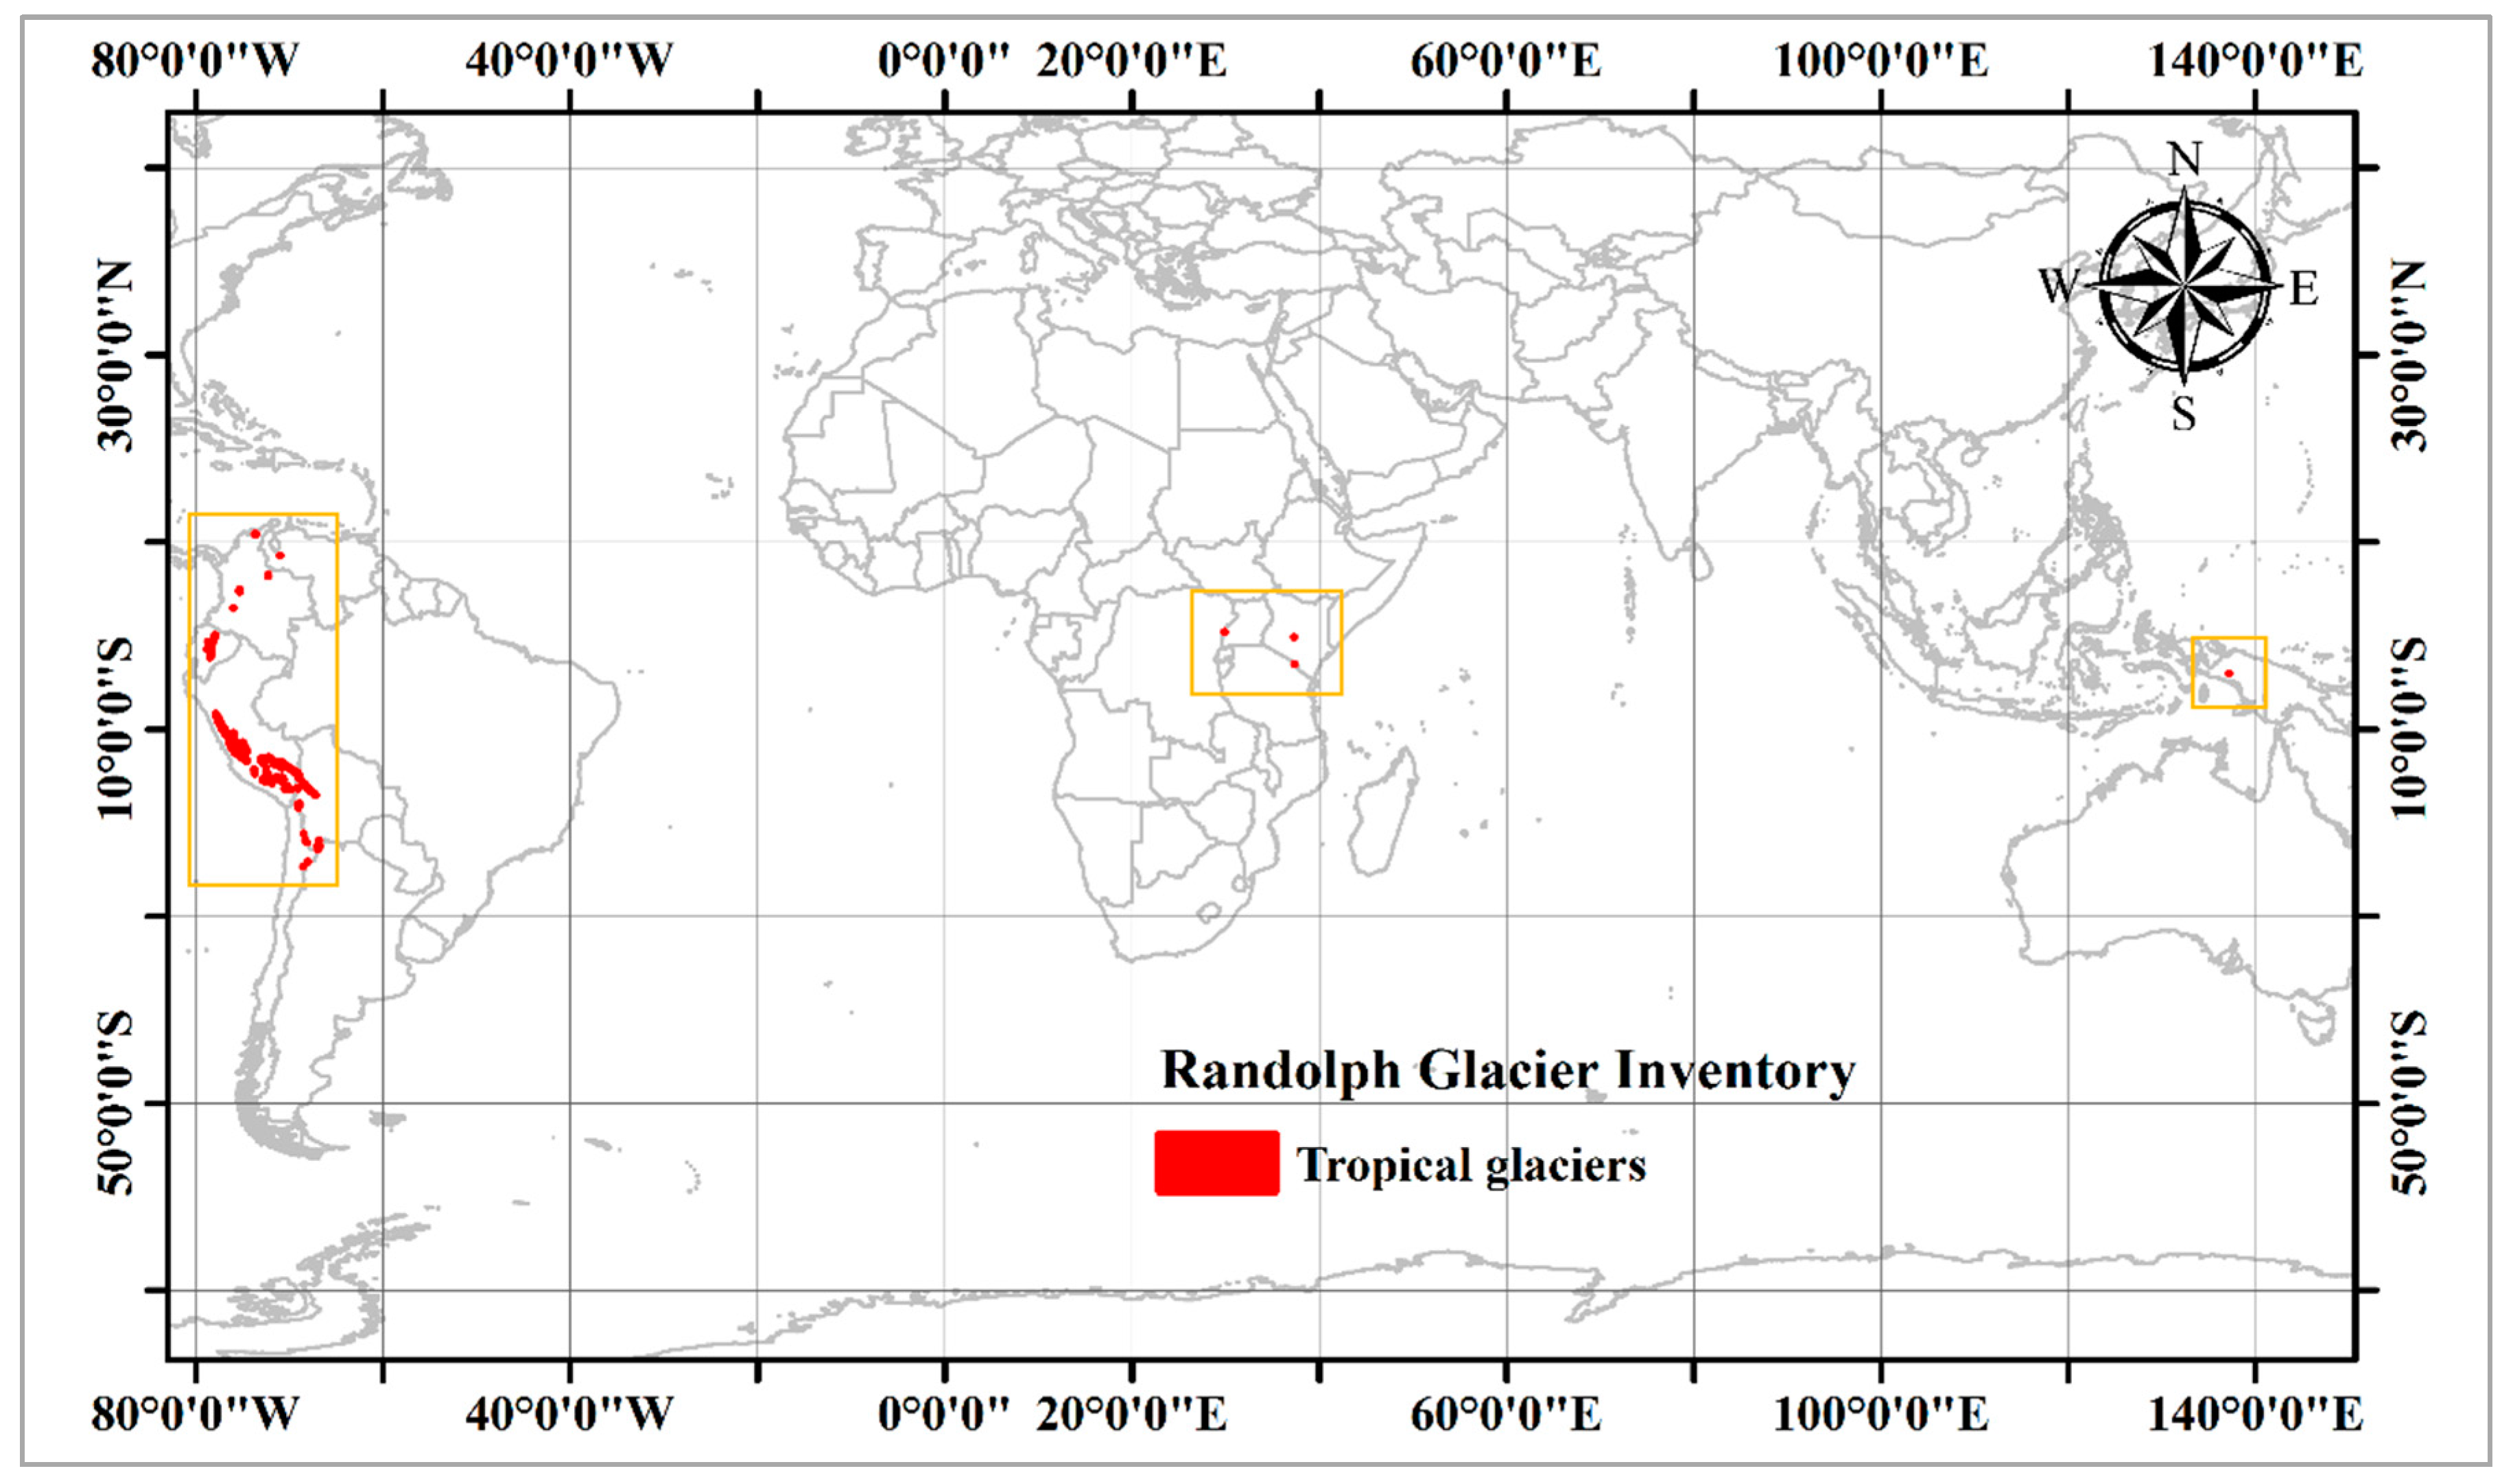
\includegraphics[width=1\textwidth]{Images/GlaciaresTropicales.png}
    \end{center}
    \caption{Distribución geográfica de los glaciares tropicales alrededor del mundo.}
    \reference{Datos tomados de \citeA{veettil2019global}.}
    \label{fig:GlaciaresTropicales}
\end{figure}

Los glaciares tropicales se denominan así debido a su ubicación cercana a la línea ecuatorial, entre el Trópico de Cáncer y el Trópico de Capricornio ($23^\circ 26'13.3'' \text{ N}$; $23^\circ 26'13.3'' \text{ S}$) (ver Figura~\ref{fig:GlaciaresTropicales}). Su ubicación los hace especialmente sensibles a las fluctuaciones climáticas, siendo incluso más susceptibles al calentamiento global que sus contrapartes en regiones polares \cite{dussaillant2019two}. Perú es el país con mayor presencia de glaciares tropicales en el mundo. Según datos del Randolph Glacier Inventory \cite{pfeffer2014randolph}, recopilados por \cite{veettil2019global}, cuenta con un total aproximado de 1602,96 km$^2$ de glaciares tropicales, lo que representa el 68.38\% del total a nivel mundial. Sin embargo, en los últimos 50 años, la superficie glaciar en el territorio peruano se ha reducido en un 53\% \cite{reserva2021}.

El Instituto Nacional de Investigación en Glaciares y Ecosistemas de Montaña (INAIGEM) es el órgano responsable del estudio y monitoreo de los glaciares y ecosistemas de montaña en Perú, y es la entidad encargada de la elaboración del Inventario Nacional de Glaciares \cite{inaigem2018inventario}.

Los inventarios de glaciares son instrumentos que forman parte de las políticas de diversos países para responder a las problemáticas relacionadas al deterioro de los ecosistemas de montaña \cite{barella2022combined}. Un inventario de glaciares proporciona información detallada del estado actual de los glaciares de una región específica a través de la recopilación de datos históricos, la delimitación y categorización de la superficie glaciar, y el posterior análisis para la elaboración de modelos predictivos que permitan identificar posibles acciones estratégicas para su conservación a través de una correcta toma de decisiones \cite{barcaza2017glacier}.

La recopilación de datos relacionados a los ecosistemas de montaña siempre se ha considerado una tarea compleja debido al difícil acceso provocado por las condiciones climáticas extremas propias del entorno y los limitados medios de transporte \cite{fang2017discriminative, nijhawan2018hybrid}. Sin embargo, la emergencia de datos provenientes de sensores remotos, en particular, las imágenes satelitales y otros productos derivados, ha simplificado significativamente este proceso \cite{gavade2021systematic}.

La implementación de técnicas de teledetección ha impulsado numerosos estudios, facilitando la adquisición y el posterior procesamiento de la información recopilada \cite{zhang2019glacier}. Entre las distintas estrategias utilizadas para esta última etapa, resalta el uso de índices espectrales. Un ejemplo notable es el Índice Normalizado de Diferencia de Nieve (NDSI, por sus siglas en inglés), el cual permite identificar las áreas cubiertas de nieve \cite{hall1995mapping}. Esto se logra mediante la diferencia normalizada entre una banda visible y una banda cercana al infrarrojo o infrarrojo de onda corta del espectro en una imagen satelital multiespectral \cite{hall2010normalized}. Además, se complementa con la definición de umbrales de valor y, en algunos casos, la discriminación visual de los resultados \cite{sibandze2014comparison, singh2021quantifying}. Países como Perú, Chile, Argentina y Colombia, han adoptado estas técnicas para la delimitación de la superficie glaciar, complementándolas con datos adicionales como modelos digitales de elevación e imágenes de alta resolución \cite{inaigem2017manual, DGA2022, castro2014manual, ospina2022metodologia}.
  
Aunque los métodos tradicionales han mostrado eficacia en la delimitación de la superficie glaciar, presentan algunas desventajas, como la tendencia a sobreestimar los resultados y una fuerte dependencia de la intervención humana debido a las limitaciones inherentes de la información espectral \cite{singh2021quantifying}.

La información espectral de una imagen satelital se deriva de la reflectancia de la superficie terrestre, que es la fracción de energía solar reflejada por la superficie y captada por los sensores del satélite \cite{chuvieco2016fundamentals}. Sin embargo, aunque este proceso es efectivo para identificar cuerpos de nieve limpios, puede verse afectado por diversos factores, como la atmósfera, la topografía, la vegetación, la nieve estacionaria, y las propiedades físicas del suelo, lo que puede generar errores en la interpretación de los datos \cite{lu2020glacier, tian2022mapping}.

Además de los desafíos previamente mencionados, surge la necesidad de identificar otros tipos de glaciares, como los glaciares cubiertos y los glaciares rocosos, los cuales presentan desafíos únicos debido a sus características particulares (ver Figura \ref{fig:ComparacionGlaciares}). Los glaciares cubiertos, tal y como su nombre lo indica, están recubiertos por una capa de escombros o rocas que pueden alterar significativamente su firma espectral, dificultando su identificación mediante métodos de teledetección tradicionales debido a su similitud con el terreno circundante \cite{zhang2019glacier}. Los glaciares rocosos, por otro lado, son glaciares compuestos por una mezcla de hielo y rocas, que al igual que los glaciares cubiertos, comparten la misma dificultad en su proceso de identificación \cite{robson2020automated}.

\begin{figure}[H]
    \begin{center}
    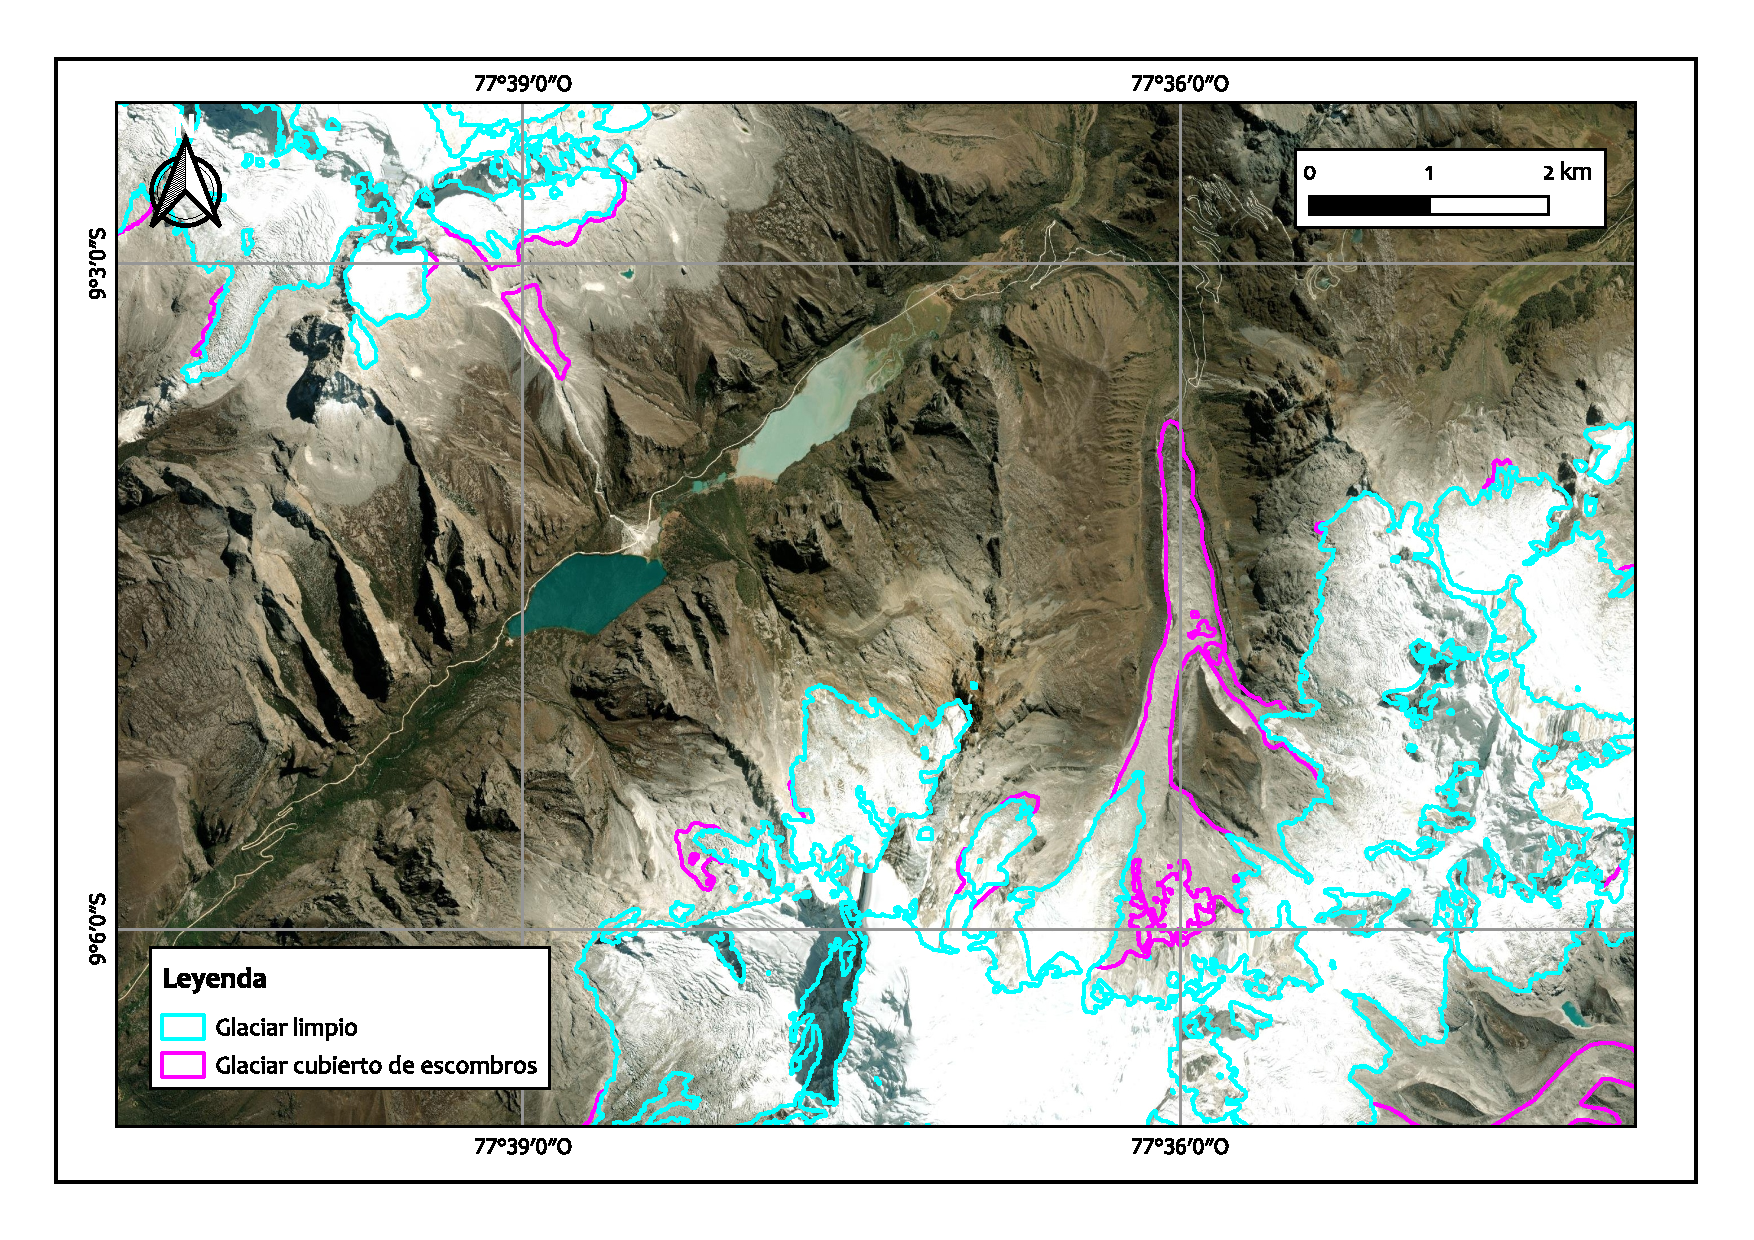
\includegraphics[width=1\textwidth]{Images/ComparacionGlaciares.pdf}
    \end{center}
    \caption{Diferencias visuales entre un glaciar limpio y un glaciar cubierto de escombros.}
    \reference{Elaborado por el autor.}
    \label{fig:ComparacionGlaciares}
\end{figure}

La importancia de la identificación de estos tipos de glaciares radica en su impacto sobre las tasas de derretimiento glaciar \cite{lu2021novel}. Los escombros delgados tienden a acelerar el derretimiento, mientras que los escombros más gruesos lo ralentizan \cite{anderson2021causes}. Además, la presencia de glaciares cubiertos también puede indicar reservas potenciales de recursos hídricos, ya que estos no están expuestos directamente a la atmósfera y por tanto, pueden retener agua de forma más efectiva \cite{zhang2019role, florath2021optical}.

Dada su semejanza espectral con el terreno circundante, la identificación de estos tipos de glaciares puede resultar en sobreestimaciones y errores en la delimitación \cite{nijhawan2018hybrid}. Los métodos tradicionales intentan abordar este desafío a través de una delimitación manual, que se basa en el uso de información adicional como imágenes de alta resolución y la obtención de parámetros morfométricos a partir de modelos digitales de elevación e imágenes satelitales de radar \cite{fang2017discriminative, lu2020glacier}. A pesar de su utilidad, este enfoque requiere una gran cantidad de experticia, y es un proceso lento, laborioso y sujeto a errores, principalmente debido a la subjetividad de la evaluación \cite{yan2021glacier, zhang2021automated, xie2022progressive, hu2022new}.

Frente a estos desafíos, las técnicas alternativas han ido ganando terreno en el ámbito de la delimitación de glaciares, destacándose en particular el Análisis de Imágenes Basado en Objetos (OBIA) y el Análisis de Imágenes Basado en Píxeles (PBIA) \cite{muhammad2013comparison, rastner2013comparison}. Sin embargo, entre estas nuevas propuestas, las técnicas que incorporan Inteligencia Artificial (IA) están cobrando una relevancia notable, gracias a su rendimiento en disciplinas de teledetección tan variadas como la agricultura, la gestión forestal y los estudios marítimos, por mencionar algunos \cite{hoeser2020object2}. Además, estas técnicas ofrecen una solución al manejo de la creciente cantidad de datos disponibles, al ser capaces de procesar grandes volúmenes de información, superando una limitación importante de los métodos tradicionales y su inherente dependencia del proceso manual \cite{lu2020glacier}.

Las técnicas más sofisticadas se valen de algoritmos fundamentados en Aprendizaje Automático y Aprendizaje Profundo \cite{xie2021evaluating}. Las metodologías que incorporan Aprendizaje Automático tienden a basarse en algoritmos como: Random Forest (RF), Support Vector Machine (SVM), o K-Nearest Neighbors (KNN), por mencionar algunos; los cuales son empleados para delimitar y clasificar superficies glaciares mediante la generación de puntos de interés, análisis espectral y características morfológicas \cite{alifu2020machine, haq2021snow}. Por otro lado, las técnicas que utilizan Aprendizaje Profundo se sustentan íntegramente en el uso de Redes Neuronales, específicamente en arquitecturas como Redes Neuronales Convolucionales, las cuales interactúan eficazmente con imágenes y permiten realizar de manera directa la segmentación semántica de los glaciares mediante el reconocimiento de patrones en los datos de entrada \cite{khan2022deep}.

La presente tesis busca incrementar la efectividad del proceso de mapeo semiautomático de glaciares limpios y cubiertos mediante el uso de imágenes satelitales. Para alcanzar este propósito, se propone el desarrollo de un modelo basado en inteligencia artificial, en particular, en técnicas de aprendizaje profundo, que posibilite la realización de una segmentación semántica precisa y óptima.

\section{Formulación del problema}
\label{sec:FormulacionProblema}

Habiendo identificado la situación problemática actual, se formula la siguiente interrogante para la investigación:

¿Cómo incrementar la efectividad del mapeo semiautomático de glaciares limpios y cubiertos en imágenes satelitales, mediante el desarrollo de un modelo de segmentación semántica basado en aprendizaje profundo?

\section{Justificación}
\label{sec:Justificacion}

\subsection{Justificación teórica}

El estudio de la superficie terrestre ha experimentado un crecimiento notable en los últimos años, impulsado por avances tecnológicos y la disponibilidad creciente de grandes volúmenes de datos \cite{hoeser2020object2}. La inteligencia artificial ha surgido como un factor crítico en este progreso, optimizando la utilización de información obtenida de sensores remotos y permitiendo la identificación más precisa y eficiente de características terrestres \cite{hoeser2020object}.

El impacto de la inteligencia artificial se ha manifestado en múltiples áreas dentro del campo de la teledetección, esto se pudo evidenciar a través del análisis de revisiones sistemáticas relacionadas al tema: \citeA{zhu2017deep, ma2019deep, yuan2020deep}.

\begin{figure}[H]
    \begin{center}
    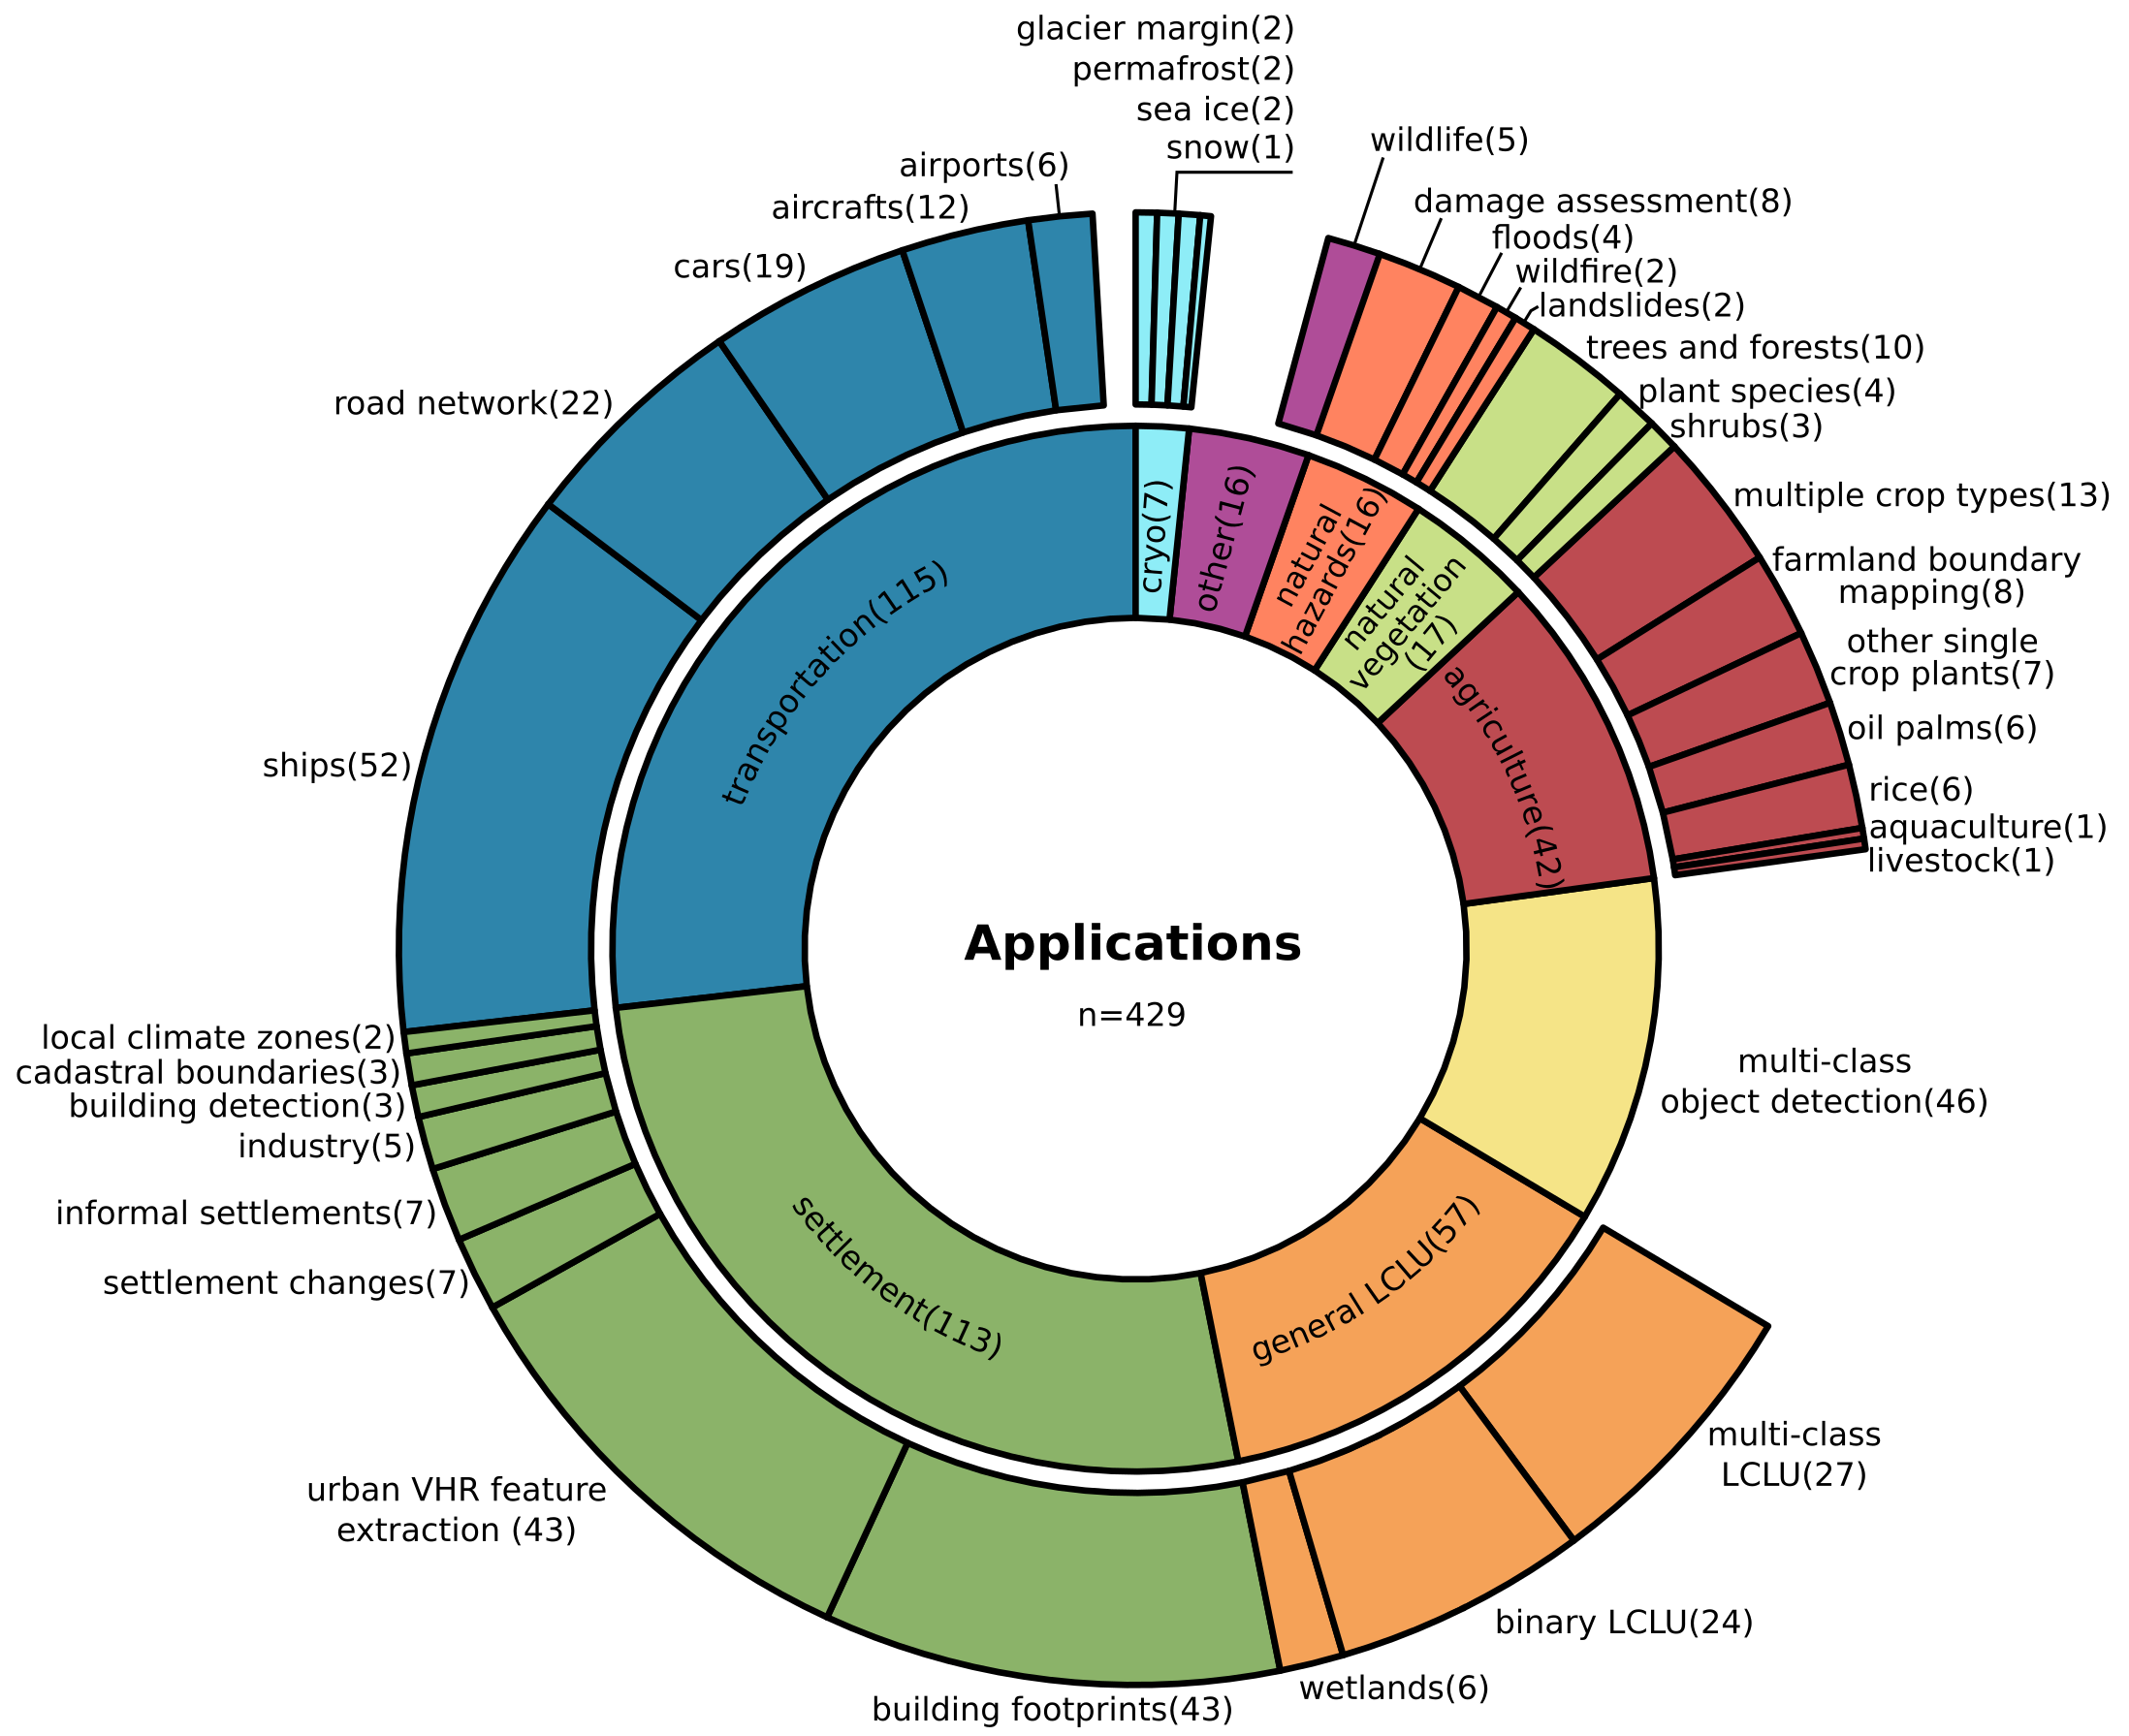
\includegraphics[width=1\textwidth]{Images/RevisionAreas.png}
    \end{center}
    \caption{Aplicaciones destacadas de la inteligencia artificial en la segmentación semántica y la detección de objetos dentro del ámbito de la teledetección.}
    \reference{Datos tomados de \citeA{hoeser2020object}.}
    \label{fig:RevisionAreas}
\end{figure}

Sin embargo, pese a los avances en la aplicación de la inteligencia artificial en la teledetección, como se evidencia en la Figura~\ref{fig:RevisionAreas}, aún se observa una representación mínima de investigaciones enfocadas en la criósfera y los ecosistemas de montaña. Este déficit puede atribuirse, en parte, a la estandarización de técnicas basadas en el cálculo de índices espectrales. Los glaciares, al poseer una firma espectral distintiva, son relativamente sencillos de detectar en comparación con otros elementos \cite{dietz2012remote}. No obstante, la complejidad emerge al mapear glaciares cubiertos de escombros o glaciares rocosos debido a sus diferencias espectrales con respecto a otros tipos de glaciares y su similitud espectral con el terreno circundante \cite{nijhawan2018hybrid}. En la actualidad, estos desafíos suelen abordarse mediante procesos manuales, tal y como se describe en la Sección~\ref{sec:SituacionProblematica}, resultando en procedimientos extensos, laboriosos y costosos.

En este contexto, la presente investigación buscará contribuir a este campo de estudio poco explorado, mediante el desarrollo de un modelo semiautomático de segmentación semántica de glaciares basado en aprendizaje profundo. Complementariamente, se efectuará una revisión sistemática de los estudios de vanguardia que incorporan inteligencia artificial en el mapeo de glaciares, con la finalidad de brindar a la comunidad científica una perspectiva actualizada de las innovaciones y tendencias emergentes en la aplicación de estas técnicas en la teledetección centrada en los ecosistemas de montaña. Se espera que estos aportes puedan impulsar nuevas investigaciones y aplicaciones basadas en inteligencia artificial en este campo, potenciando la capacidad para monitorizar y entender los cambios y dinámicas en los ecosistemas de montaña.

\subsection{Justificación práctica}

En América Latina, países como Perú, Chile, Argentina y Colombia disponen de instituciones especializadas en el estudio y seguimiento de glaciares y ecosistemas de montaña \cite{inaigem2017manual, DGA2022, castro2014manual, ospina2022metodologia}. Estas entidades cuentan con equipos multidisciplinarios responsables de la creación de sus respectivos inventarios de glaciares.

Los inventarios de glaciares son instrumentos cruciales para las administraciones gubernamentales a nivel mundial, facilitando la implementación de políticas de respuesta al rápido declive de la superficie glaciar en regiones específicas \cite{barella2022combined}. La actualización constante de estos inventarios es esencial, puesto que la calidad y la contemporaneidad de los datos tienen una incidencia directa en la eficacia de las estrategias para la conservación de los glaciares \cite{alifu2020machine, lu2021novel, xie2022progressive}.

Sin embargo, la actualización de un inventario de glaciares es un proceso largo y costoso debido a su inherente complejidad \cite{yan2021glacier}. Este proceso comprende varias etapas, incluyendo la recopilación de información histórica y geoespacial, el análisis de gabinete, la validación en campo, y finalmente, la publicación de los resultados \cite{barcaza2017glacier}. Es por tal motivo que países como Perú han establecido un intervalo de actualización de cinco años para su inventario de glaciares \cite{inaigem2018inventario}, lo que supone una desventaja considerando que, el 86\% de los glaciares en Perú posee una superficie menor a 1 $km^2$, siendo los más susceptibles a los efectos del cambio climático. \cite{reserva2021}.

En ese contexto, la presente investigación busca aportar en la optimización del uso de recursos mediante el incremento de la efectividad en el mapeo semiautomático de glaciares limpios y cubiertos mediante el desarrollo un modelo de segmentación semántica basado en aprendizaje profundo.

Se busca, además, establecer un punto de referencia para la adaptación de nuevas técnicas basadas en el uso de inteligencia artificial en las metodologías empleadas para la elaboración de inventarios de glaciares en los países de la región.

\section{Objetivos}
\label{sec:Objetivos}

\subsection{Objetivo general}

Incrementar la efectividad del mapeo semiautomático de glaciares limpios y cubiertos en imágenes satelitales mediante el desarrollo de un modelo de segmentación semántica basado en aprendizaje profundo.

\subsection{Objetivos específicos}

\begin{itemize}
   \item OE1: Realizar una revisión sistemática de la literatura sobre el estado del arte de la segmentación semántica de glaciares en imágenes satelitales que hagan uso de técnicas basadas en aprendizaje automático y aprendizaje profundo.
   \item OE2: Construir un conjunto de datos para el entrenamiento y validación del modelo propuesto a partir de la recopilación de imágenes satelitáles multiespectrales y modelos digitales de elevación.
   \item OE3: Desarrollar un modelo de segmentación semántica basado en aprendizaje profundo para el mapeo de  glaciares limpios y cubiertos, haciendo uso del conjunto de datos previamente creado.
   \item OE4: Evaluar la efectividad del modelo desarrollado y realizar una comparación de su desempeño con modelos existentes utilizando métricas adecuadas para la evaluación de tareas de segmentación semántica.
   \item OE5: Analizar los resultados obtenidos para identificar las ventajas y desventajas del modelo propuesto, con el fin de explorar posibles aplicaciones en otros campos de estudio.
\end{itemize}

\section{Propuesta}
\label{sec:Propuesta}

Desarrollar un modelo de segmentación semántica basado en aprendizaje profundo para incrementar la efectividad en el mapeo semiautomático de glaciares limpios y cubiertos en imágenes satelitales.

\section{Hipótesis}
\label{sec:Hipotesis}

El desarrollo de un modelo de segmentación semántica basado en aprendizaje profundo incrementará la efectividad del mapeo semiautomático de glaciares limpios y cubiertos en imágenes satelitales.

\section{Variables}
\label{sec:Variables}

\subsection{Variable independiente}

\textbf{Modelo de segmentación semántica basado en aprendizaje profundo}: El desarrollo de un modelo de segmentación semántica basado en aprendizaje profundo es la variable independiente en este estudio. Esta variable representa el factor que se modificará y controlará para analizar su efecto en la efectividad del mapeo de glaciares limpios y cubiertos en imágenes satelitales.

\subsection{Variable dependiente}

\textbf{Efectividad del mapeo de glaciares limpios y cubiertos en imágenes satelitales}: La efectividad del mapeo de glaciares limpios y cubiertos en imágenes satelitales es la variable dependiente en este estudio. Esta variable representa el resultado que se medirá y analizará para evaluar cómo es afectada por el uso del modelo de segmentación semántica basado en aprendizaje profundo.  

\section{Operacionalización de variables}
\label{sec:OperacionalizacionVariables}

El Cuadro~\ref{tab:OperacionalizacionVariables} se muestra la operacionalización de las variables de investigación.

\begin{landscape}
\begin{table}
\caption{Operacionalización de variables de la investigación}
\footnotesize
\begin{tabularx}{\linewidth}{@{} *5{X} @{}}
\hline
\textbf{Variables} & \textbf{Tipo} & \textbf{Dimensión} & \textbf{Indicadores} \\ \hline
\multirow{11}{=}{\parbox{4cm}{Modelo de segmentación semántica basado en aprendizaje profundo}} & \multirow{11}{=}{\parbox{4cm}{Variable independiente}} & \multirow{4}{=}{\parbox{4cm}{Arquitectura del modelo}} & - Número de capas. \\ &  &  & - Número de parámetros. \\
 &  &  & - Tasa de aprendizaje. \\
 &  &  & - Función de pérdida. \\ \cline{3-4}
 &  & Función de activación & - Función de activación utilizada en las capas ocultas. \\ \cline{3-4}
 &  & Algoritmo de optimización & - Algoritmo utilizado para optimizar el modelo. \\ \cline{3-4}
 &  & \multirow{5}{*}{Conjunto de datos} & - Número de muestras. \\
 &  &  & - Número de muestras utilizadas en el entrenamiento. \\
 &  &  & - Número de muestras utilizadas en la validación. \\
 &  &  & - Número de canales. \\
 &  &  & - Número de clases. \\ \hline
\multirow{8}{=}{\parbox{4cm}{Efectividad del mapeo de glaciares limpios y cubiertos en imágenes satelitales}} & \multirow{8}{=}{\parbox{4cm}{Variable dependiente}} & \multirow{6}{=}{\parbox{4cm}{Precisión}} & - IoU. \\
 &  &  & - Dice. \\
 &  &  & - Accuracy. \\
 &  &  & - Precision. \\
 &  &  & - Recall. \\
 &  &  & - F1 Score. \\ \cline{3-4} 
 &  & Tiempo & - Tiempo requerido para la segmentación semántica en la etapa de pruebas. \\ \cline{3-4}
 &  & Calidad & - Porcentaje de error en la delimitación de glaciares. \\ \hline
\end{tabularx}
\begin{minipage}{\textwidth}
    \vspace{10pt}
    \reference{Elaborado por el autor.}
    \label{tab:OperacionalizacionVariables}
\end{minipage}
\end{table}
\end{landscape}


\section{Organización del documento}
\label{sec:OrganizacionDocumento}

La presente tesis cuenta con un total de siete capítulos, organizados de la siguiente manera:

El \textit{Capítulo~\ref{chp:MarcoTeorico}} establece el marco teórico, proporcionando los fundamentos de la investigación. En este capítulo, se exploran las bases teóricas y se examinan los antecedentes relevantes que respaldan el estudio.

El \textit{Capítulo~\ref{chp:Metodologia}} describe la metodología utilizada en esta investigación. En este capítulo, se especifica el tipo y diseño de la investigación, la unidad de análisis, la población estudiada y el tamaño de la muestra. Además, se exponen las técnicas empleadas para la recopilación de datos.

El \textit{Capítulo~\ref{chp:Propuesta}} expone la propuesta de investigación, detallando los pasos que se han seguido para la creación, desarrollo y ejecución del modelo de segmentación semántica basado en aprendizaje profundo.

El \textit{Capítulo 5} está dedicado a la exposición, interpretación y discusión de los resultados obtenidos de la investigación.

El \textit{Capítulo 6} presenta las conclusiones de la investigación. En este capítulo, se sintetizan los hallazgos y se responden a los objetivos inicialmente planteados.

El \textit{Capítulo 7} recoge las recomendaciones resultantes de la investigación y se señalan posibles futuras líneas de investigación para ampliar el estudio del tema abordado.

\chapter{MARCO TEÓRICO}
\label{chp:MarcoTeorico}
\thispagestyle{fancy} % Aplica el estilo de página a la primera página del capítulo.

\section{Antecedentes de investigación}
\label{sec:AntecedentesInvestigacion}

\subsection{Revisión sistemática de la literatura}
\label{suc:RevisionSistematicaLiteratura}

Una revisión sistemática de la literatura es un proceso objetivo que implica recopilar, sintetizar y analizar estudios primarios, tanto desde una perspectiva cuantitativa como cualitativa. Su objetivo principal es resumir de manera rigurosa la información existente sobre un tema específico, identificando tendencias, brechas en el conocimiento y áreas de investigación futura \cite{aromataris2014systematic}. Esta metodología contribuye al avance del campo en cuestión al proporcionar una comprensión profunda y completa de la temática analizada. Además, se considera que una revisión sistemática de la literatura es fundamental para la toma de decisiones informadas y la generación de conocimiento basado en evidencia científica \cite{manterola2013revisiones}.

El primer paso en la realización de la presente revisión sistemática de la literatura fue establecer una metodología de trabajo. Para ello, se analizaron diversas opciones, como la metodología PRISMA, desarrollada por \cite{moher2009preferred}, y sus posteriores actualizaciones. Sin embargo, se decidió adoptar la metodología propuesta por \cite{2007Kitchenham} como base metodológica de la presente revisión sistemática de la literatura debido a su aplicabilidad en el área de ingeniería de software y ciencias de la computación \cite{2019Bajaj, carrera2022context}.

Tal y como se muestra en la Figura~\ref{fig:RSL}, esta metodología se compone de tres fases: la planificación, la ejecución y el informe de la revisión sistemática de la literatura.

\begin{figure}[H]
    \begin{center}
    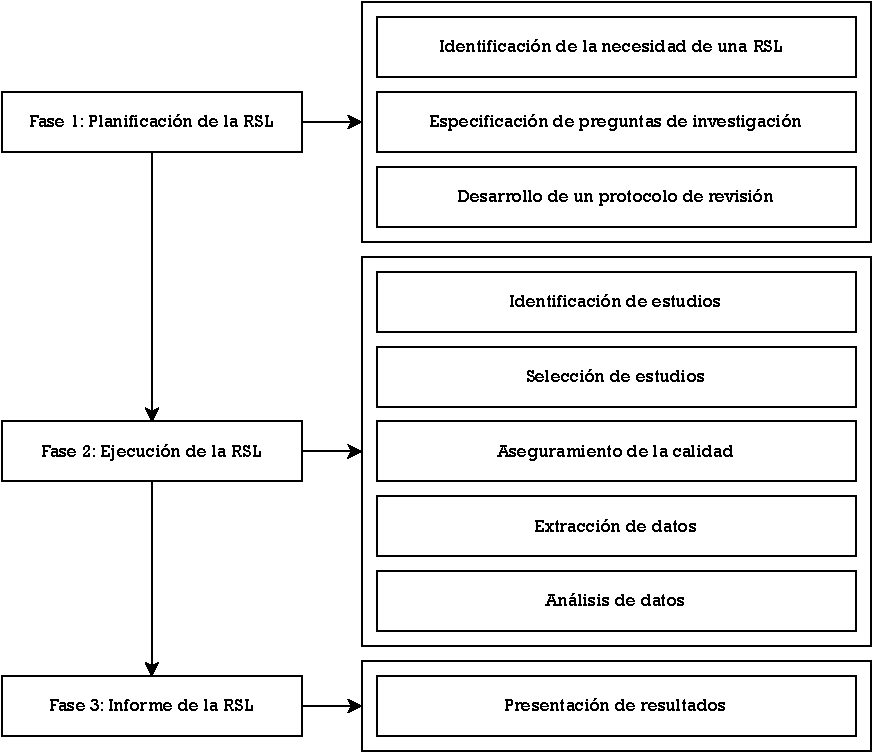
\includegraphics[width=1\textwidth]{Images/RSL.pdf}
    \end{center}
    \caption{Proceso de revisión sistemática de la literatura (RSL).}
    \reference{Elaborado por el autor.}
     \label{fig:RSL}
\end{figure}

\subsubsection{Fase 1: Planificación de la revisión sistemática de la literatura}

\textit{Necesidad de una revisión sistemática de la literatura}

A través del análisis de diversas revisiones sistemáticas, se ha evidenciado un marcado aumento en las propuestas basadas en la aplicación de inteligencia artificial en problemas relacionados con la teledetección \cite{zhu2017deep, ma2019deep, yuan2020deep}. Tanto el aprendizaje automático como el aprendizaje profundo se han convertido, en los últimos años, en las técnicas predilectas para abordar problemas comunes en el campo de la teledetección, tal y como se puede apreciar en la Figura~\ref{fig:DeepLearningRemoteSensing}.

\begin{figure}[H]
    \begin{center}
    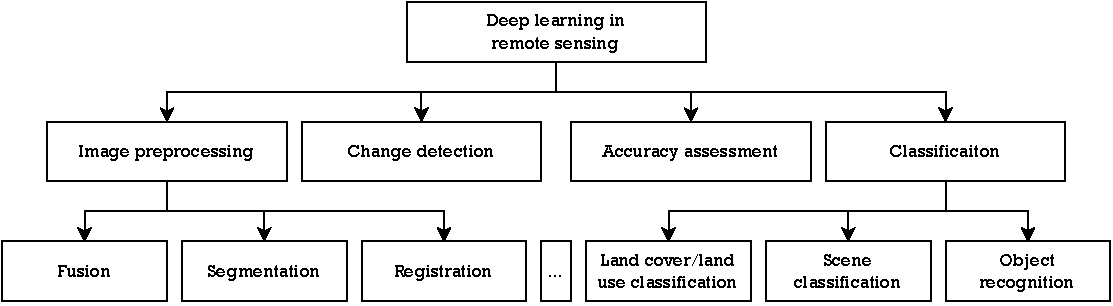
\includegraphics[width=1\textwidth]{Images/DeepLearningRemoteSensing.pdf}
    \end{center}
    \caption{Taxonomía de las principales aplicaciones del aprendizaje profundo en el campo de la teledetección.}
    \reference{Datos tomados de \citeA{ma2019deep}.}
     \label{fig:DeepLearningRemoteSensing}
\end{figure}

Algunas revisiones sistemáticas se centran en el estudio y recopilación de información relevante sobre la aplicación del aprendizaje profundo en tareas específicas, como la detección y segmentación de objetos. Un ejemplo destacado de tales revisiones sistemáticas son los trabajos propuestos por \citeA{hoeser2020object} y \citeA{hoeser2020object2}. Otras revisiones se enfocan en la aplicación de un algoritmo específico como Random Forest o Support Vector Machines en el campo de la teledetección \cite{mountrakis2011support, belgiu2016random}.

Por otro lado, también se han identificado revisiones sistemáticas que abordan un campo de aplicación en particular, en lugar de analizar tareas específicas. Tal es el caso de \citeA{khelifi2020deep}, en donde se aborda la aplicación del aprendizaje profundo para la detección de cambios; o los propuestos por \citeA{yasir2023ship, er2023ship}, revisiones sistemáticas que se enfocan en analizar las diferentes técnicas basadas en aprendizaje profundo para la detección de barcos en imágenes satelitales ópticas e imágenes de radar de apertura sintética (SAR).

En la actualidad, existe una escasez de revisiones sistemáticas centradas específicamente en el uso de inteligencia artificial para el mapeo de glaciares. Por ejemplo, el trabajo de \citeA{kaushik2019development}, detalla la aplicación de diversas técnicas basadas en aprendizaje automático en la región correspondiente a la India del Himalaya. En su revisión, se destacan el uso de algoritmos de aprendizaje profundo para el mapeo de glaciares cubiertos de escombros y la utilización de modelos digitales de elevación e imágenes de radar. También se resalta la problemática asociada a la delimitación manual de glaciares y la dependencia de imágenes de alta resolución.

Otra revisión, realizada por \citeA{liu2021review}, recopila los principales estudios que han empleado aprendizaje profundo en el estudio de la criósfera, abordando su aplicación en el estudio de glaciares, capas de hielo, permafrost, nieve, hielo marino y hielo de río. Es relevante mencionar que algunas revisiones analizan el impacto del aprendizaje profundo en el estudio de los ecosistemas de montaña. Sin embargo, estas revisiones no se enfocan en el mapeo de glaciares, sino más bien en la estimación de masa glaciar y el monitoreo de parámetros glaciares, como señala \citeA{bhardwaj2022applications}.

La búsqueda de revisiones sistemáticas ha revelado que los estudios sobre glaciares generalmente se abordan como parte de una revisión más general. Un ejemplo de ello es la revisión sistemática propuesta por \citeA{han2023survey}, cuyo enfoque se centra en el análisis de cinco aplicaciones de teledetección en entornos geológicos: litología, presencia de agua, tipos de suelo, glaciares rocosos y cartografía de desastres geológicos.

A pesar de que algunos estudios de revisión sistemática han abordado la temática del mapeo de glaciares mediante inteligencia artificial, la literatura en este campo sigue siendo limitada. Por lo tanto, existe una oportunidad y una necesidad para llevar a cabo una revisión sistemática que se centre específicamente en el uso de técnicas de inteligencia artificial para el mapeo y la cartografía de glaciares, abordando los desafíos y avances recientes en este ámbito.

\textit{Objetivo de investigación}

El objetivo de esta revisión sistemática es realizar un análisis de los estudios que emplean algoritmos de aprendizaje automático y aprendizaje profundo en el mapeo de glaciares mediante el uso de imágenes satelitales. Se busca recopilar, evaluar y sintetizar la literatura científica actual sobre esta temática para identificar los enfoques más efectivos y comprender cómo han contribuido al avance del conocimiento en el campo del monitoreo glaciar.

Para definir el alcance de la revisión sistemática, se ha adoptado un enfoque basado en el marco de trabajo PICOC (Población, Intervención, Comparación, Resultados y Contexto), detallado en el Cuadro~\ref{tab:PicocCriteria}.

\begin{table}[H]
\small
\caption{Utilización del criterio PICOC para definir el alcance y objetivo de la revisión sistemática de la literatura (RSL).\label{tab:PicocCriteria}}
\newcolumntype{C}{>{\centering\arraybackslash}X}
\begin{tabularx}{\textwidth}{lX}
\hline
\textbf{Criterio} & \textbf{Descripción}\\
\hline
(\textit{P}) Población & Glaciares. \\ \hline
(\textit{I}) Intervención & Algoritmos de aprendizaje automático y aprendizaje profundo.\\ \hline
(\textit{C}) Comparación & No aplica (no se realizará comparación con otro tipo de intervención).\\ \hline
(\textit{O}) Resultado & Mapeo de glaciares.\\ \hline
(\textit{C}) Contexto & Uso de imágenes satelitales.\\
\hline
\end{tabularx}
\reference{Elaborado por el autor.}
\end{table}

\textit{Preguntas de investigación}

Se han identificado un total de seis preguntas de investigación derivadas directamente del objetivo y los alcances previamente definidos mediante el marco de trabajo PICOC. La lista de preguntas, junto con su correspondiente motivación, se encuentra detallada en la Tabla \ref{tab:PreguntasInvestigacion}.

\begin{table}[H]
\small
\caption{Preguntas de investigación.}
\begin{tabularx}{\textwidth}{lXX}
\hline
\textbf{No.} & \textbf{Pregunta} & \textbf{Motivación}\\
\hline
RQ1	& ¿Cuáles fueron las técnicas específicas de aprendizaje automático o aprendizaje profundo utilizadas en el mapeo de glaciares?	& Identificar y catalogar las técnicas existentes para comprender el estado actual del uso de aprendizaje automático y aprendizaje profundo en el mapeo de glaciares en la literatura. \\\hline
RQ2	& ¿Cuáles fueron las métricas de evaluación empleadas para cuantificar el rendimiento de las técnicas aplicadas en el mapeo de glaciares?	& Evaluar la efectividad y comparar los resultados de las técnicas de mapeo de glaciares mediante el análisis de las métricas de evaluación utilizadas en estudios previos. \\\hline
RQ3	& ¿Cuáles fueron las principales fuentes de imágenes satelitales utilizadas para realizar el mapeo de glaciares?	& Identificar las fuentes de datos satelitales más comúnmente utilizadas en la literatura para obtener imágenes de glaciares y evaluar su disponibilidad y aplicabilidad. \\\hline
RQ4	& ¿Cómo se construyó el conjunto de datos utilizado para la aplicación de las técnicas de aprendizaje automático o aprendizaje profundo en el mapeo de glaciares?	& Comprender la metodología utilizada para recopilar y preparar el conjunto de datos de entrenamiento y prueba, incluyendo el tamaño del conjunto de datos, la selección de muestras representativas y la estrategia de etiquetado. \\\hline
RQ5	& ¿Qué tipos de glaciares se buscaron mapear en el contexto de la investigación? & Identificar y clasificar los diferentes tipos de glaciares abordados en la literatura para comprender las características y particularidades de cada tipo y su relevancia en el contexto científico. \\\hline
RQ6	& ¿Cuál fue la región geográfica donde se llevó a cabo el mapeo de glaciares? & Identificar y delimitar las regiones geográficas específicas donde se centró el mapeo de glaciares en los estudios revisados, lo cual puede tener implicaciones en términos de variabilidad geográfica y aplicabilidad de los resultados. \\
\hline
\end{tabularx}
\reference{Elaborado por el autor.}
\label{tab:PreguntasInvestigacion}
\end{table}

\textit{Protocolo de revisión}

% TODO: Agregar mas fuentes que enumeren revistas o fuentes de búsqueda para RS.
\textbf{Selección de fuentes bibliográficas:} La selección de fuentes bibliográficas se basó en el análisis de revisiones sistemáticas previas relacionadas con la aplicación de inteligencia artificial en el campo de la teledetección. Estas revisiones sistemáticas, como las propuestas por \citeA{khelifi2020deep}, permitieron identificar y recopilar las principales bases de datos relevantes para la investigación (ver Cuadro~\ref{tab:SeleccionFuentes}).

\begin{table}[H]
\small
\caption{Fuentes bibliográficas.}
\begin{tabularx}{\textwidth}{XlXp{2cm}}
\hline
\textbf{Base de datos} & \textbf{URL} & \textbf{Área} & \textbf{Búsqueda avanzada S/N}\\
\hline
arXiv &
\href{https://arxiv.org}{https://arxiv.org} & Interdisciplinario & S \textsuperscript{*}\\\hline
IEEE Xplore &
\href{https://ieeexplore.ieee.org}{https://ieeexplore.ieee.org} & Tecnología & S\\\hline
MDPI &
\href{https://mdpi.com}{https://mdpi.com} & Interdisciplinario & S \textsuperscript{*}\\\hline
Nature &
\href{https://nature.com}{https://nature.com} & Interdisciplinario & S \textsuperscript{*}\\\hline
Science Direct &
\href{https://sciencedirect.com}{https://sciencedirect.com} & Interdisciplinario & S\\\hline
Scopus &
\href{https://scopus.com}{https://scopus.com} & Interdisciplinario & S\\\hline
Springer Link &
\href{https://link.springer.com}{https://link.springer.com} & Interdisciplinario & S \textsuperscript{*}\\\hline
Taylor \& Francis &
\href{https://tandfonline.com}{https://tandfonline.com} & Interdisciplinario & S\\\hline
Web of Science &
\href{https://webofscience.com}{https://webofscience.com} & Interdisciplinario & S\\
\hline
\end{tabularx}
\noindent{\footnotesize{\textsuperscript{*} Cadena de búsqueda no disponible.}}
\vspace{0.25cm}
\newline
\reference{Elaborado por el autor.}
\label{tab:SeleccionFuentes}
\end{table}

\textbf{Criterios de inclusión y exclusión:} Con el objetivo de identificar los estudios más relevantes, se propusieron criterios de inclusión y exclusión, los cuales se detallan en el Cuadro~\ref{tab:CriteriosSeleccion}.

\begin{table}[H]
\small
\caption{Criterios de selección.\label{tab:CriteriosSeleccion}}
\newcolumntype{C}{>{\centering\arraybackslash}X}
\begin{tabularx}{\textwidth}{XX}
\hline
\textbf{Criterio de inclusión} & \textbf{Criterio de exclusión}\\
\hline
Estudios enfocados a los ecosistemas de montaña (glaciares limpios, cubiertos o de roca). & Estudios cuyo enfoque principal no es el mapeo de glaciares.\\\hline
Estudios que aplicaron IA (aprendizaje automático/profundo) para el mapeo de glaciares. & Estudios que no hicieron uso de imágenes satelitales.\\\hline
Estudios disponibles, escritos en inglés, con un identificador válido. & Estudios comparativos o revisiones o que no presenten métricas de evaluación. \\
\hline
\end{tabularx}
\reference{Elaborado por el autor.}
\end{table}

La selección de estos criterios se realizó con el propósito de alinear la revisión sistemática con el objetivo inicialmente planteado. Se incluyeron aquellos estudios centrados en el mapeo de glaciares de montaña, siempre y cuando emplearan técnicas basadas en inteligencia artificial, ya sea aprendizaje automático o aprendizaje profundo, sin importar la región geográfica o el tipo de glaciar según su contenido de impurezas (glaciares limpios, glaciares cubiertos de escombros, glaciares rocosos). Se consideraron únicamente los estudios escritos en inglés, que estuvieran disponibles y que contaran con un identificador de indexación válido (DOI).

Por otro lado, se excluyeron los trabajos cuyo enfoque principal no estuviera directamente relacionado con el mapeo de glaciares, como estudios de dinámica glacial, análisis de cambios temporales, generación de inventarios y estudios ambientales, por mencionar algunos. Aquellos estudios que no hubieran utilizado imágenes satelitales, o que se enfocaran exclusivamente en la comparación de algoritmos sin proponer modificaciones, así como revisiones sistemáticas o trabajos que no presentaran métricas de evaluación, también fueron excluidos de la revisión sistemática.

El proceso de selección se llevó a cabo en dos etapas: la primera incluyó un filtro inicial en el que se seleccionaron los estudios publicados en los últimos 5 años, es decir, a partir del año 2017, con el objetivo de obtener información actualizada sobre nuevos algoritmos y determinar las tendencias futuras en la aplicación de nuevas metodologías. Esta etapa incluyó una revisión rápida de títulos y resúmenes basada en los criterios de selección previamente establecidos en el Cuadro~\ref{tab:CriteriosSeleccion}. La segunda etapa comprendió la revisión detallada de cada estudio para decidir su inclusión o exclusión según el cumplimiento de los criterios de selección.

\textbf{Aseguramiento de la calidad:} En base a revisiones sistemáticas anteriores \cite{2019Bajaj}, se ha decidido llevar a cabo una evaluación de la calidad de los estudios mediante las siguientes preguntas:

\begin{table}[H]
\small
\caption{Aseguramiento de la calidad.}
\begin{tabularx}{\textwidth}{lX}
\hline
\textbf{No.} & \textbf{Pregunta}\\
\hline
QA1 & ¿Los objetivos y el propósito de la investigación están claramente definidos en el estudio analizado? \\ \hline
QA2 & ¿El estudio presenta una explicación clara de los datos empleados, así como el número total de imágenes recopiladas para la investigación? \\ \hline
QA3 & ¿El estudio presenta una explicación clara del algoritmo propuesto para el mapeo de glaciares? \\ \hline
QA4 & ¿El estudio presenta un diagrama explicativo que ilustra la metodología utilizada y define claramente los pasos seguidos en la investigación? \\ \hline
QA5 & ¿El estudio proporciona acceso público al código fuente y los datos utilizados en la investigación? \\
\hline
\end{tabularx}
\reference{Elaborado por el autor.}
\label{tab:AseguramientoCalidad}
\end{table}

De acuerdo con el Cuadro~\ref{tab:AseguramientoCalidad}, se estableció un sistema de puntuación para cada pregunta: 0 (No), 0.5 (Parcialmente) y 1 (Sí). Así, un trabajo que cumplió con todos los criterios obtuvo una puntuación máxima de 5. Los trabajos que no alcanzaron al menos una puntuación de 2.5 fueron excluidos del proceso de selección. Esta metodología tuvo como objetivo garantizar la calidad de los estudios seleccionados, asegurando que solo se incluyeran en la revisión sistemática aquellos que satisficieron los criterios establecidos.

\textbf{Extracción de datos:} En el proceso de extracción de datos, se empleó una estructura que recopilaba la siguiente información:

\begin{table}[H]
\small
\caption{Extracción de datos.}
\begin{tabularx}{\textwidth}{lXp{4.8cm}}
\hline
\textbf{Categoría} & \textbf{Descripción} & \textbf{Sub categoría}\\
\hline
Datos bibliográficos & Información básica del estudio, como autor(es), año de publicación y fuente de publicación. & DOI. Título. Año. Tipo de publicación. Fuente de publicación. Autores. País de afiliación del primer autor. Número de citas. Número de referencias. \\ \hline
Conjunto de datos & Detalles sobre el origen y características del conjunto de datos utilizado en el estudio. & Inventarios consultados. Sensor de origen. Bandas utilizadas. Número de imágenes. Número de muestras. Distribución. Disponibilidad de descarga. \\ \hline
Glaciares & Información específica sobre los glaciares identificados en el estudio, incluyendo su ubicación geográfica. & Tipo de glaciar. Región geográfica. \\ \hline
Metodología & Descripción detallada del algoritmo propuesto para el mapeo de glaciares y la metodología utilizada en la investigación. & Algoritmo(s) propuesto(s). Tipo de problema. Diagrama de la metodología. Disponibilidad de código fuente. Ventajas. Limitaciones. Trabajos futuros.\\ \hline
Evaluación & Detalles sobre el proceso de evaluación de cada estudio, incluyendo los resultados y las métricas utilizadas. & Métricas. Resultados. Comparación con otros estudios. \\ \hline
\end{tabularx}
\reference{Elaborado por el autor.}
\label{tab:ExtracionDatos}
\end{table}

Todas estas categorías de información se relacionaron estrechamente con la respuesta a las preguntas de investigación detalladas en el Cuadro~\ref{tab:PreguntasInvestigacion}, así como con las preguntas de seguimiento de la calidad especificadas en el Cuadro~\ref{tab:AseguramientoCalidad}. Además, se buscó identificar las ventajas y limitaciones de cada estudio, así como los trabajos futuros propuestos por los autores.

\textbf{Estrategia de búsqueda:} Se emplearon dos estrategias de búsqueda en la presente revisión sistemática: una búsqueda primaria y una búsqueda secundaria.

\textit{Búsqueda Primaria}: En la búsqueda primaria, el enfoque principal fue emplear una cadena de búsqueda específica en diversas bases de datos, las cuales habían sido previamente identificadas y descritas en el Cuadro~\ref{tab:SeleccionFuentes}.

La cadena de búsqueda empleada fue la siguiente: \textit{(glacier'' OR glacial'') AND (mapping'' OR delineation'' OR detection'' OR segmentation'') AND (artificial intelligence'' OR machine learning'' OR ``deep learning'')}.

% TODO: Agregar mas referencias en la ultima cita.
El diseño de la cadena de búsqueda se basó en las sugerencias hechas por \cite{buckley2005towards}, las cuales se resumen en el Cuadro~\ref{tab:EstrategiaBusquedaPrimaria}, y que han sido utilizadas en otras revisiones sistemáticas, como las desarrolladas por \citeA{2019Bajaj}.

\begin{table}[H] 
\small
\caption{Estrategia de búsqueda primaria.\label{tab:EstrategiaBusquedaPrimaria}}
\newcolumntype{C}{>{\centering\arraybackslash}X}
\begin{tabularx}{\textwidth}{p{4.25cm}X}
\hline
Identificar palabras clave & Palabras clave obtenidas a partir del análisis PICOC y de las preguntas de investigación. Estas fueron  ``glacier'', ``mapping'', ``artificial intelligence''.\\\hline
Identificar sinónimos, abreviaturas, o palabras relacionadas a las palabras clave &
Palabras estrechamente relacionadas a las palabras clave identificadas previamente, estas pueden incluir sinónimos, abreviaturas o acrónimos. Estas fueron  ``glacial'' de parte de la palabra ``glacier'', se consideraron sinónimos de ``mapping'' como ``delineation'' , ``detection'' , y ``segmentation'', así mismo, se consideraron parabras relacionadas a ``artificial intelligence'' como ``machine learning'' y ``deep learning''.\\\hline
Buscar conectores para palabras clave & Palabras que se empleen coomo conectores de las palabras clave. Se emplearon dos conectores, OR para alternativas, sinónimos, abreviaturas o acrónimos, y AND como enlaces filtros de las palabras clave. \\\hline
Construir cadenas de búsqueda específicas & Construcción de cadenas de búsqueda específicas para cada base de datos que incluyan las palabras clave y los operadores correspondientes.\\
\hline
\end{tabularx}
\reference{Elaborado por el autor.}
\end{table}

\textit{Búsqueda Secundaria}: La búsqueda secundaria consistió en analizar las referencias bibliográficas de cada estudio seleccionado, así como las citas realizadas por otros autores a dichos estudios. El propósito de esta estrategia fue identificar posibles trabajos adicionales que fueran relevantes y pudieran ser incorporados en la revisión sistemática. Esta metodología amplió el alcance de la revisión y aseguró que se consideraran estudios adicionales que aportaran valor y complementaran la investigación.

\subsubsection{Fase 2: Ejecución de la revisión sistemática de la literatura}

\textit{Ejecución de la búsqueda}

La ejecución de la búsqueda se llevó a cabo aplicando tanto la cadena de búsqueda primaria como las cadenas de búsqueda específicas detalladas en el Cuadro~\ref{tab:CadenasBusquedaEspecifica}.

\begin{table}[H]
\small
\caption{Cadenas de búsquedas específicas.\label{tab:CadenasBusquedaEspecifica}}
\newcolumntype{C}{>{\centering\arraybackslash}X}
\begin{tabularx}{\textwidth}{lX}
\hline
IEEE Xplore & ((((((``Document Title'': glacier OR glacial) AND (``All Metadata'': artificial intelligence OR machine learning OR deep learning) AND (``All Metadata'': mapping OR segmentation OR detection OR delineation)))))). \\\hline
Scopus & TITLE (glacier OR glacial) AND ALL (``mapping'' OR ``segmentation'' OR ``detection'' OR ``delineation'') AND ALL (``artificial intelligence'' OR ``machine learning'' OR ``deep learning''). \\\hline
Web of Science & TI=(glacier OR glacial) AND ALL=(``mapping'' OR ``segmentation'' OR ``detection'' OR ``delineation'') AND ALL=(``artificial intelligence'' OR ``machine learning'' OR ``deep learning''). \\\hline
Taylor \& Francis & [[Publication Title: glacier] OR [Publication Title: glacial]] AND [[All: ``mapping''] OR [All: ``segmentation''] OR [All: ``detection''] OR [All: ``delineation'']] AND [[All: ``artificial intelligence''] OR [All: ``machine learning''] OR [All: ``deep learning'']]. \\
\hline
\end{tabularx}
\reference{Elaborado por el autor.}
\end{table}

Las cadenas de búsqueda específicas se diseñaron para búsquedas avanzadas en bases de datos que ofrecían esta opción, como se detalla en el Cuadro~\ref{tab:SeleccionFuentes}. En cuanto a las demás bases de datos, se recurrió a sus herramientas de búsqueda integradas, que comúnmente se presentaban como formularios de búsqueda avanzada. Los valores introducidos en estos formularios se derivaron de la cadena de búsqueda principal.

\textit{Identificación de estudios}

La búsqueda inicial arrojó un total de 431 estudios. La distribución de estos, según la base de datos consultada, se detalla en el Cuadro~\ref{tab:ResultadoPrimario}.

\begin{table}[H]
\small
\caption{Resultados preliminares de la identificación de estudios.}
\begin{tabularx}{\textwidth}{p{8.5cm}c}
\hline
\textbf{Base de datos} & \textbf{N° de estudios encontrados}\\
\hline
arXiv & 5 \\\hline
IEEE Xplore & 15 \\\hline
MDPI & 27 \\\hline
Nature & 22 \\\hline
Science Direct & 50 \\\hline
Scopus & 252 \\\hline
Springer Link & 16 \\\hline
Taylor \& Francis & 9 \\\hline
Web of Science & 35 \\
\hline
\end{tabularx}
\reference{Elaborado por el autor.}
\label{tab:ResultadoPrimario}
\end{table}

A través de la búsqueda de duplicados, se excluyeron 124 estudios identificados por tener el mismo identificador (DOI). Posteriormente, se utilizó la API de \href{https://www.crossref.org}{Crossref} para obtener los metadatos de los estudios restantes. Sin embargo, 7 de ellos no contaban con metadatos registrados en dicha plataforma. Debido a esto, se decidió excluirlos temporalmente, aunque fueron analizados durante el proceso de búsqueda secundaria. El proceso completo de identificación, selección y aseguramiento de la calidad de la revisión sistemática se detalla en la Figura~\ref{fig:ResumenRevision}.

\begin{figure}[H]
    \begin{center}
    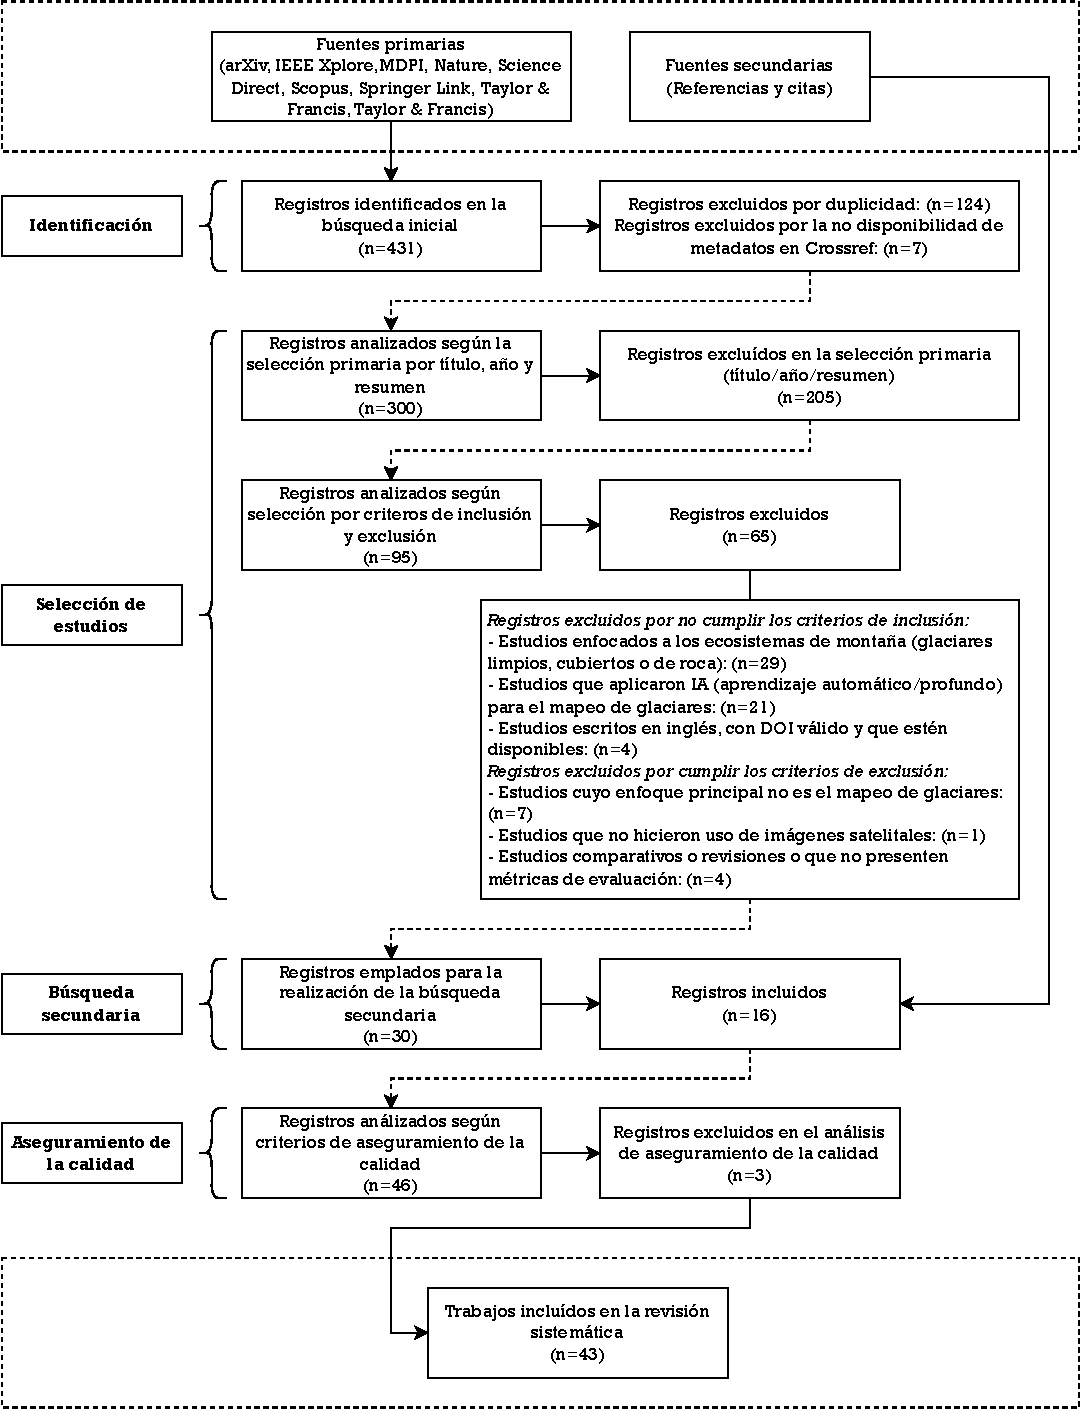
\includegraphics[width=1\textwidth]{Images/ResumenRevision.pdf}
    \end{center}
    \caption{Proceso de identificación y selección de estudios para la revisión sistemática de la literatura.}
    \reference{Elaborado por el autor.}
    \label{fig:ResumenRevision}
\end{figure}

\textit{Selección de estudios}

\textbf{Selección inicial:} 

El proceso inició con un total de 300 estudios identificados. En la primera etapa de selección, se revisaron los títulos y, cuando fue necesario, los resúmenes de cada documento. De estos, se identificaron 205 trabajos vinculados a diversas temáticas, como el análisis histórico del cambio en la cobertura glaciar \cite{kumar2020lake} \cite{intsiful2020glacier} \cite{wang2021current}, análisis de ecosistemas de la criósfera \cite{bourquin2022microbiome}, o el estudio de la cinemática glaciar \cite{dematteis2021ten} \cite{groh2019rock}. No obstante, varios de estos trabajos no se encontraban en consonancia con los criterios de búsqueda o no se alineaban con el objetivo principal de la revisión sistemática, razón por la cual fueron excluidos.

\textbf{Selección basada en criterios de inclusión y exclusión}: Contrario a la etapa anterior, en este paso se llevó a cabo una revisión detallada, aunque ágil, del contenido íntegro de cada documento, atendiendo a los criterios de inclusión y exclusión especificados en el Cuadro~\ref{tab:CriteriosSeleccion}.

Se identificaron 29 trabajos que no se centraban en el estudio de ecosistemas de montaña. En su mayoría, estos estudios estaban relacionados con la identificación de frentes de desprendimiento glaciar, localizados principalmente en la Antártida o en regiones del Ártico. De igual manera, 17 trabajos no se alineaban con el uso de técnicas basadas en inteligencia artificial, ya sea aprendizaje automático o aprendizaje profundo. En su lugar, estos estudios proponían técnicas alternativas como el análisis basado en píxeles (PBIA) o el análisis basado en objetos (OBIA).

Por otro lado, se excluyeron 7 trabajos cuyo enfoque no estaba directamente relacionado con el mapeo de glaciares. Adicionalmente, se descartó un estudio que no empleaba imágenes satelitales \cite{kattenborn2019convolutional}. Algunos trabajos enfocaron su metodología en la comparación de algoritmos de aprendizaje automático y aprendizaje profundo \cite{khan2020machine, xie2021evaluating}. Sin embargo, otros trabajos o no presentaban métricas de evaluación o simplemente se limitaban a describir la situación actual en forma de revisión literaria \cite{kaushik2019development}.

En total, 65 documentos fueron excluidos en esta fase. Como resultado final del proceso de búsqueda primaria, se obtuvieron 30 estudios que sirvieron como entrada para la siguiente etapa.

\textit{Búsqueda secundaria}

Esta búsqueda consistió en revisar las referencias y citas de los 30 estudios identificados en la búsqueda primaria. Es importante destacar que, aunque la búsqueda primaria se llevó a cabo en septiembre del año 2022, la revisión de las citas permitió actualizar la revisión sistemática con trabajos publicados hasta el primer semestre del año 2023. Al igual que en la etapa anterior, se buscó automatizar parcialmente este proceso a través de la consulta del API de Crossref para obtener referencias y de la plataforma \href{https://www.scite.ai}{Scite} para las citas. Inicialmente, se identificaron 846 referencias y 168 citas, descartando previamente aquellos trabajos ya analizados en la búsqueda primaria o que estaban duplicados. Tras combinar estas referencias y citas, se obtuvo un total de 1010 estudios, una vez eliminados los duplicados del conjunto total.

A partir de aquí se siguió un proceso similar al de la búsqueda primaria. Se descartaron aquellos trabajos publicados antes del año 2017 (499). Adicionalmente, se excluyeron 333 trabajos cuyo título no contenía la palabra ``glacier''. De este modo, 178 documentos fueron evaluados conforme a los criterios de selección del Cuadro~\ref{tab:CriteriosSeleccion}.

Contrario a la búsqueda primaria, en esta ocasión se observó una baja incidencia de trabajos no asociados a ecosistemas de montaña (11). Sin embargo, sobresalió la cantidad de estudios, 119 en total, que no implementaron técnicas de inteligencia artificial. Esta diferencia puede atribuirse al orden en que se aplicaron los criterios. Por tanto, dentro de esos 119 estudios que no recurrieron a la inteligencia artificial, es posible encontrar investigaciones que tampoco abordaron el mapeo de glaciares o que no se valieron de imágenes satelitales.

Finalmente, mediante el proceso de búsqueda secundaria, se incorporaron 15 trabajos a la revisión sistemática. Sin embargo, se llevó a cabo un análisis adicional de los estudios cuyos metadatos no se pudieron obtener automáticamente a través de la API de Crossref. De este conjunto reducido de 14 estudios, se decidió incluir el trabajo propuesto por \citeA{baraka2020machine}. Por lo tanto, el resultado final del proceso de selección fue de 46 estudios (30 a través de la búsqueda primaria y 16 a través de la búsqueda secundaria).

\textit{Aseguramiento de la calidad}

En esta fase, los estudios fueron sometidos a una evaluación de calidad basada en los criterios establecidos en el Cuadro~\ref{tab:AseguramientoCalidad} y el sistema de puntuación descrito anteriormente. Siguiendo este enfoque, los trabajos que no alcanzaron una puntuación de 2.5 fueron excluidos de la revisión sistemática. Los resultados de esta evaluación se presentan en el Cuadro~\ref{tab:AseguramientoCalidadResultado}.

Los criterios para evaluar la calidad de los trabajos se basaron en su habilidad para responder adecuadamente a las preguntas de investigación. Era vital verificar que cada estudio tuviera objetivos bien definidos y que su metodología estuviera detalladamente descrita. En estas investigaciones, se dio importancia a la inclusión de diagramas metodológicos que mostraran el proceso completo. Se consideró tanto la naturaleza de los datos utilizados como la capacidad del autor para explicar las técnicas propuestas.

En relación con la disponibilidad de información adicional, como el conjunto de datos y el código fuente, este aspecto no es siempre esencial en otras revisiones sistemáticas. No obstante, en este contexto, se valoró por su relevancia en la reproducibilidad y transparencia de los resultados. Algunos estudios indicaron que esta información podría obtenerse contactando a los autores, mientras que otros señalaron que no era pertinente. Los estudios que ofrecieron tanto el conjunto de datos como el código fuente recibieron una puntuación de 1, y aquellos que proporcionaron solo uno de estos elementos, 0.5.

\begin{table}[H]
\small
\caption{Resultados obtenidos en el proceso de aseguramiento de la calidad.}
\begin{tabularx}{\textwidth}{cX}
\hline
\textbf{Puntuación} & \textbf{Artículos de investigación}\\
\hline
1.5 & \cite{10.1109/multi-temp.2017.8035233} \\ \hline
2.0 & \cite{ayma2019mapping}, \cite{10.5194/isprs-annals-v-3-2020-417-2020} \\ \hline
2.5 & \cite{fang2017discriminative}, \cite{thanki2019glacier}, \cite{yan2020automatic}, \cite{ambinakudige2022estimation}, \cite{shukla2022super} \\ \hline
3.0 & \cite{wang2020glacier} \\ \hline
3.5 & \cite{alifu2020machine}, \cite{khan2020machine}, \cite{haq2021snow}, \cite{florath2022glacier}, \cite{lin2022accurate}, \cite{roberts2022changes}, \cite{tian2022mapping}, \cite{su142013485} \\ \hline
4.0 & \cite{nijhawan2018hybrid}, \cite{patel2019mapping}, \cite{zhang2019glacier}, \cite{robson2020automated}, \cite{he2020glacier}, \cite{lu2020glacier}, \cite{marcer2020rock}, \cite{xie2020glaciernet}, \cite{xie2020upward}, \cite{lu2021novel}, \cite{pandey2021integrated},\cite{yan2021glacier}, \cite{barella2022combined}, \cite{hu2022new}, \cite{khan2022deep}, \cite{panwar2022classification}, \cite{sharda2022hybrid}, \cite{xie2022glaciernet2}, \cite{xie2022progressive}, \cite{yao2022potential}, \cite{xiao2023glacier}, \cite{yang2023delineation} \\ \hline
4.5 & \cite{chen2022long}, \cite{chu2022glacier}, \cite{erharter2022machine}, \cite{aryal2023boundary}, \cite{thomas2023integrated} \\ \hline
5.0 & \cite{baraka2020machine}, \cite{hu2022mapping} \\
\hline
\end{tabularx}
\reference{Elaborado por el autor.}
\label{tab:AseguramientoCalidadResultado}
\end{table}

A partir de esta evaluación, se decidió excluir aquellos trabajos con una puntuación de 1.5 y 2. Dichos estudios no ofrecían una representación gráfica a través de un diagrama metodológico, carecían de detalles específicos sobre el conjunto de datos (lo cual dificultaría la respuesta a las preguntas de investigación relacionadas) y no proporcionaban información adicional.

\textit{Extracción de datos}

Para recabar datos de los estudios seleccionados, se implementaron dos métodos de recolección: uno basado en la obtención de información bibliográfica mediante búsqueda automatizada usando la API de Crossref, y otro a través de cuestionarios que abordaban las preguntas de investigación y las definidas en el proceso de aseguramiento de calidad, como se detalla en el Cuadro~\ref{tab:ExtracionDatos}. 

Antes de implementar estos métodos, se confirmó que todos los estudios proporcionaran información, ya fuera de manera íntegra o parcial, conforme a los criterios preestablecidos. Esto se logró mediante procesos previos de selección fundamentados en criterios de inclusión y exclusión, así como el análisis de aseguramiento de la calidad. La información recabada sirvió para responder a las preguntas de investigación y complementar la revisión sistemática en cuanto a las tendencias en la aplicación de estos métodos. Además, se identificaron áreas de oportunidad para futuros trabajos y posibles mejoras.
 
\textit{Análisis de datos}

\textit{Análisis de datos}

Tras extraer los datos, estos fueron procesados y almacenados en archivos CSV, facilitando su manejo con herramientas como Pandas y Plotly en Python. En primer lugar, se examinó la información bibliográfica para identificar elementos clave, como las principales fuentes de información, conferencias, revistas de investigación y la evolución en la publicación de estudios relacionados con el uso de aprendizaje automático o profundo en el mapeo de glaciares de montaña.

La Figura~\ref{fig:ArticuloAnio} muestra una tendencia al alza en la cantidad de investigaciones sobre el tema. Sin embargo, el año 2021 presentó una reducción en las publicaciones. Cabe destacar que este estudio se llevó a cabo durante el primer semestre de 2023, lo que podría explicar la disminución de artículos respecto a años anteriores. En resumen, se observa un crecimiento sostenido en la producción de investigaciones a lo largo del tiempo.

\begin{figure}[H]
    \begin{center}
    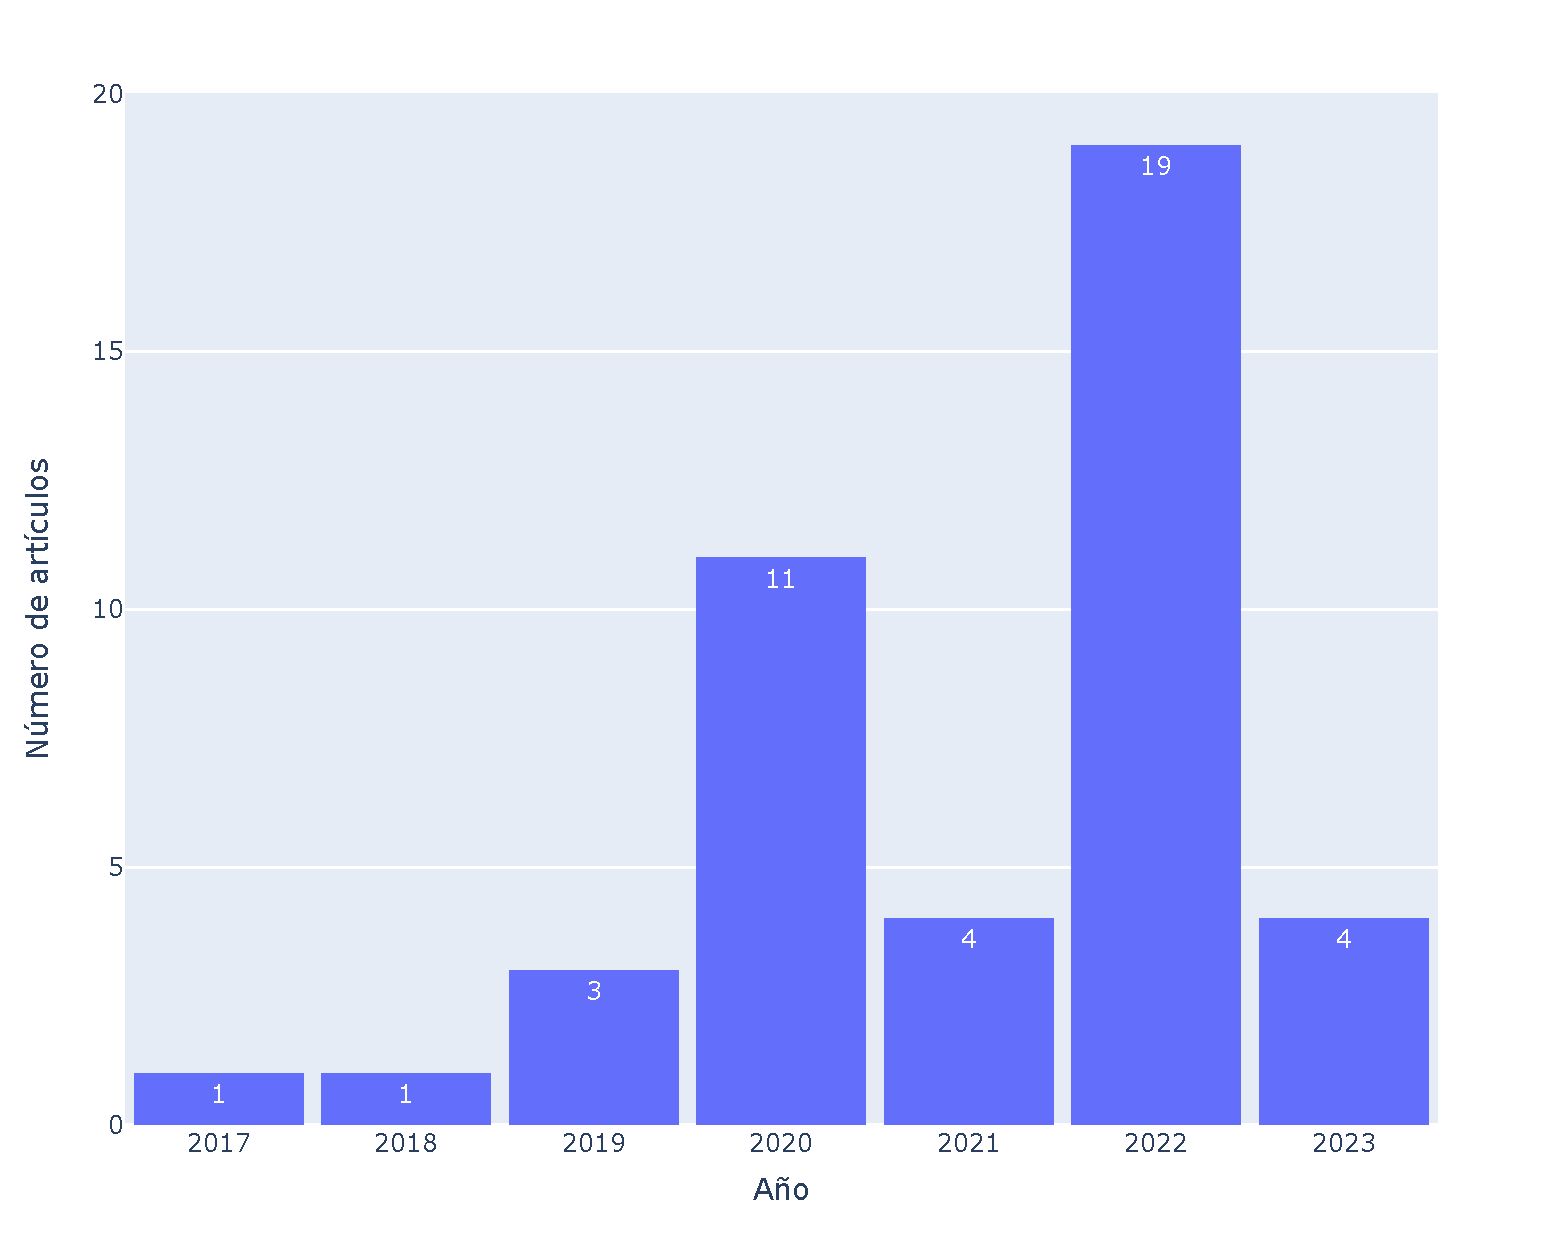
\includegraphics[width=0.75\textwidth]{Images/ArticuloAnio.pdf}
    \end{center}
    \caption{Artículos publicados entre 2017 y 2023 sobre mapeo de glaciares de montaña en imágenes satelitales con aprendizaje automático y aprendizaje profundo.}
    \reference{Elaborado por el autor.}
     \label{fig:ArticuloAnio}
\end{figure}

Posteriormente, se identificaron los países de afiliación de los primeros autores de cada artículo. Este análisis arrojó luz sobre las regiones donde se realizó la investigación e, indirectamente, sobre las áreas geográficas abordadas en los estudios. Esta información permitió dar a conocer qué países están contribuyendo activamente en el ámbito del mapeo de glaciares de montaña mediante técnicas de aprendizaje automático y profundo. Conforme a lo detallado en la Figura~\ref{fig:ArticuloPaises}, China lidera en cantidad de publicaciones en este campo, seguido de India y Estados Unidos, además de varios países de Europa y Asia.

\begin{figure}[H]
    \begin{center}
    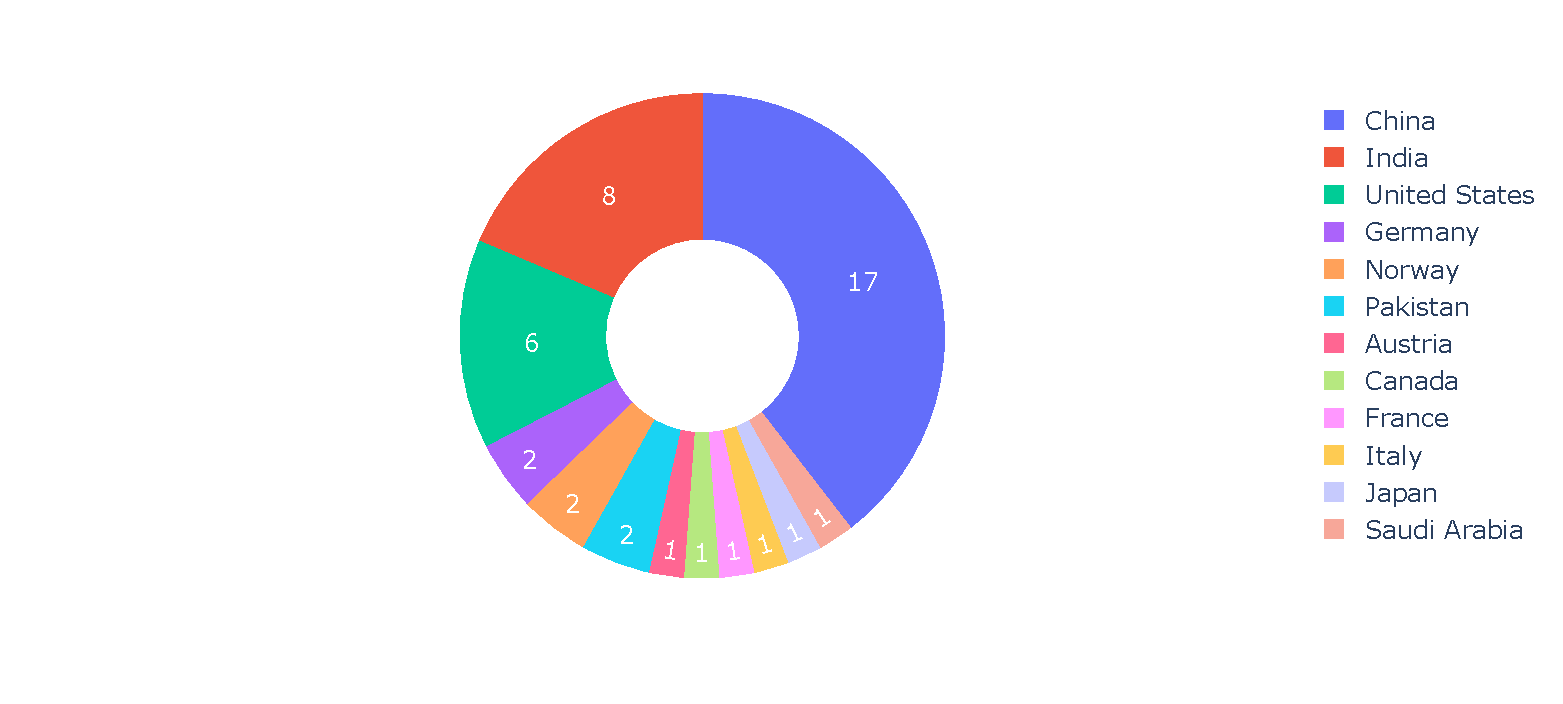
\includegraphics[width=1\textwidth]{Images/ArticuloPaises.pdf}
    \end{center}
    \caption{Artículos sobre mapeo de glaciares de montaña en imágenes satelitales con aprendizaje automático y aprendizaje profundo, según el país de la afiliación del primer autor.}
    \reference{Elaborado por el autor.}
     \label{fig:ArticuloPaises}
\end{figure}

La Figura~\ref{fig:ArticuloPaisesMapa} presenta la distribución geográfica de las investigaciones identificadas en esta revisión sistemática. Se destaca la presencia de países asiáticos como China, Pakistán e India, como se mencionó anteriormente.

\begin{figure}[H]
    \begin{center}
    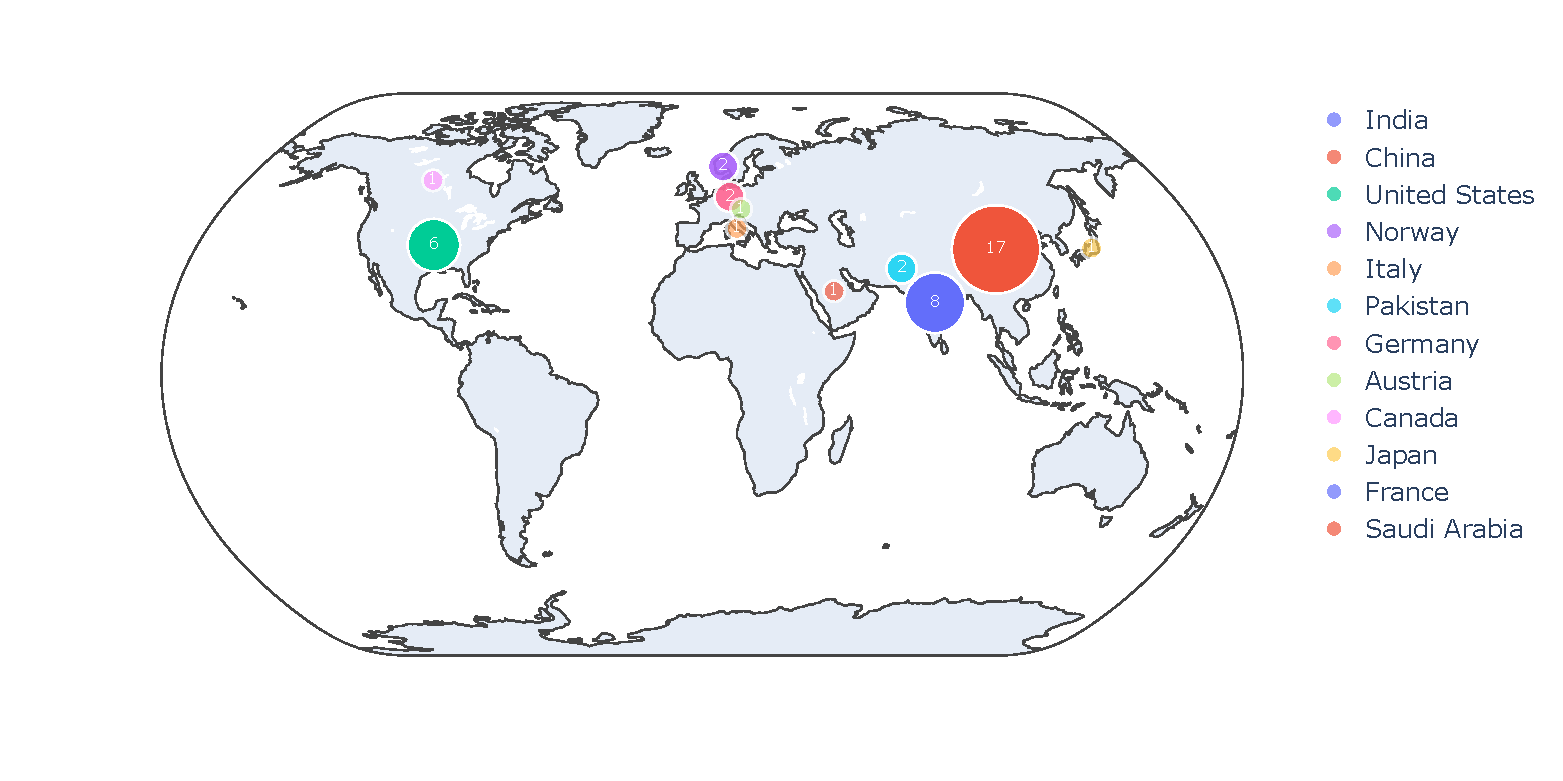
\includegraphics[width=1\textwidth]{Images/ArticuloPaisesMapa.pdf}
    \end{center}
    \caption{Distribución geográfica de artículos sobre mapeo de glaciares de montaña en imágenes satelitales con aprendizaje automático y aprendizaje profundo.}
     \label{fig:ArticuloPaisesMapa}
\end{figure}

Como siguiente paso, se determinó la cantidad de artículos de investigación publicados en revistas científicas en comparación con los presentados en conferencias o congresos académicos (ver Figura~\ref{fig:ArticuloTipo}). Este análisis mostró cómo se distribuyen las publicaciones entre estos dos medios académicos, ofreciendo una visión más clara sobre la difusión de avances en el mapeo de glaciares de montaña mediante técnicas de aprendizaje automático y aprendizaje profundo.

\begin{figure}[H]
    \begin{center}
    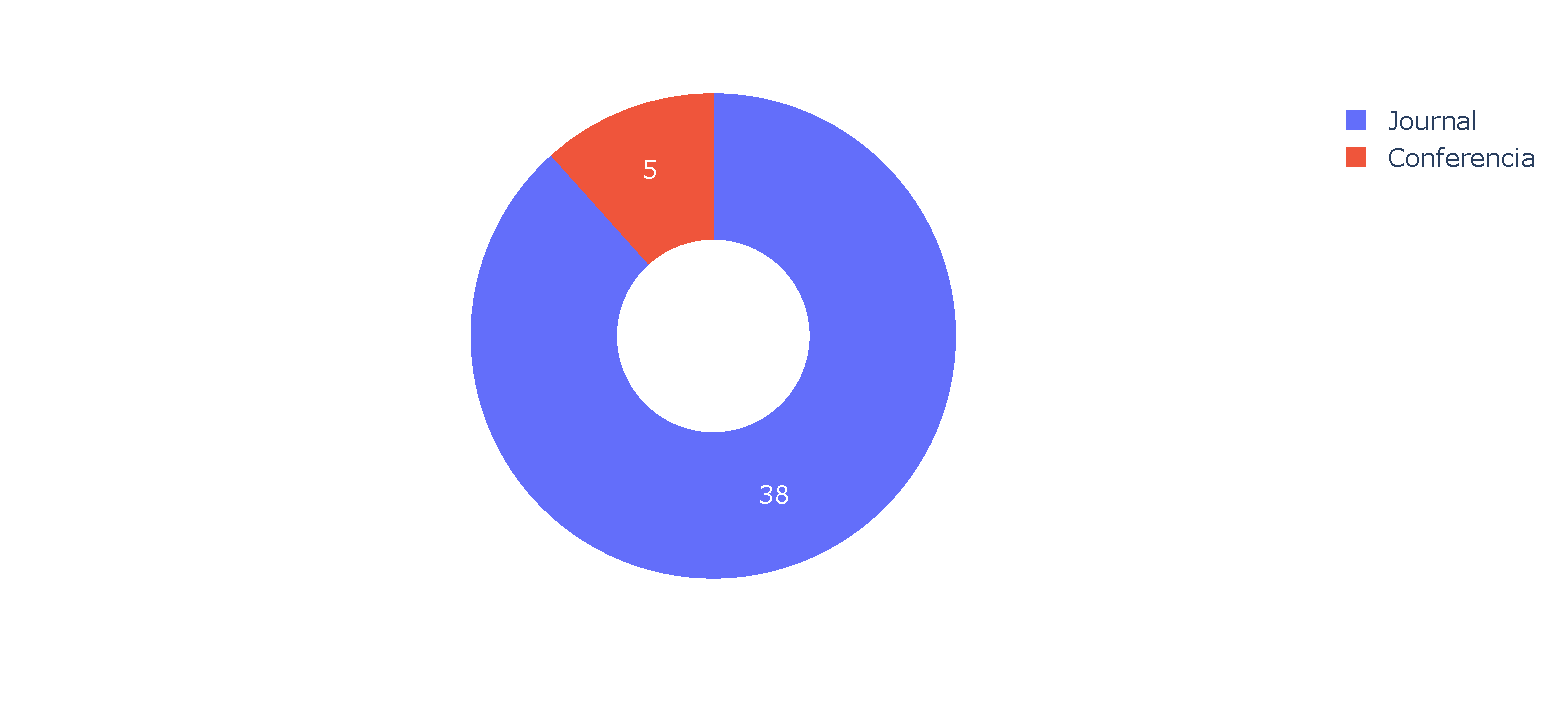
\includegraphics[width=1\textwidth]{Images/ArticuloTipo.pdf}
    \end{center}
    \caption{Artículos sobre mapeo de glaciares montaña en imágenes satelitales con aprendizaje automático y profundo, publicados en revistas científicas o conferencias académicas.}
     \label{fig:ArticuloTipo}
\end{figure}

Por último, y tomando como referencia otras revisiones sistemáticas como \citeA{2019Bajaj, hoeser2020object2}, se detalló la fuente donde se hallaron los estudios vinculados al mapeo de glaciares de montaña en imágenes satelitales mediante aprendizaje automático y aprendizaje profundo.

\begin{figure}[H]
    \begin{center}
    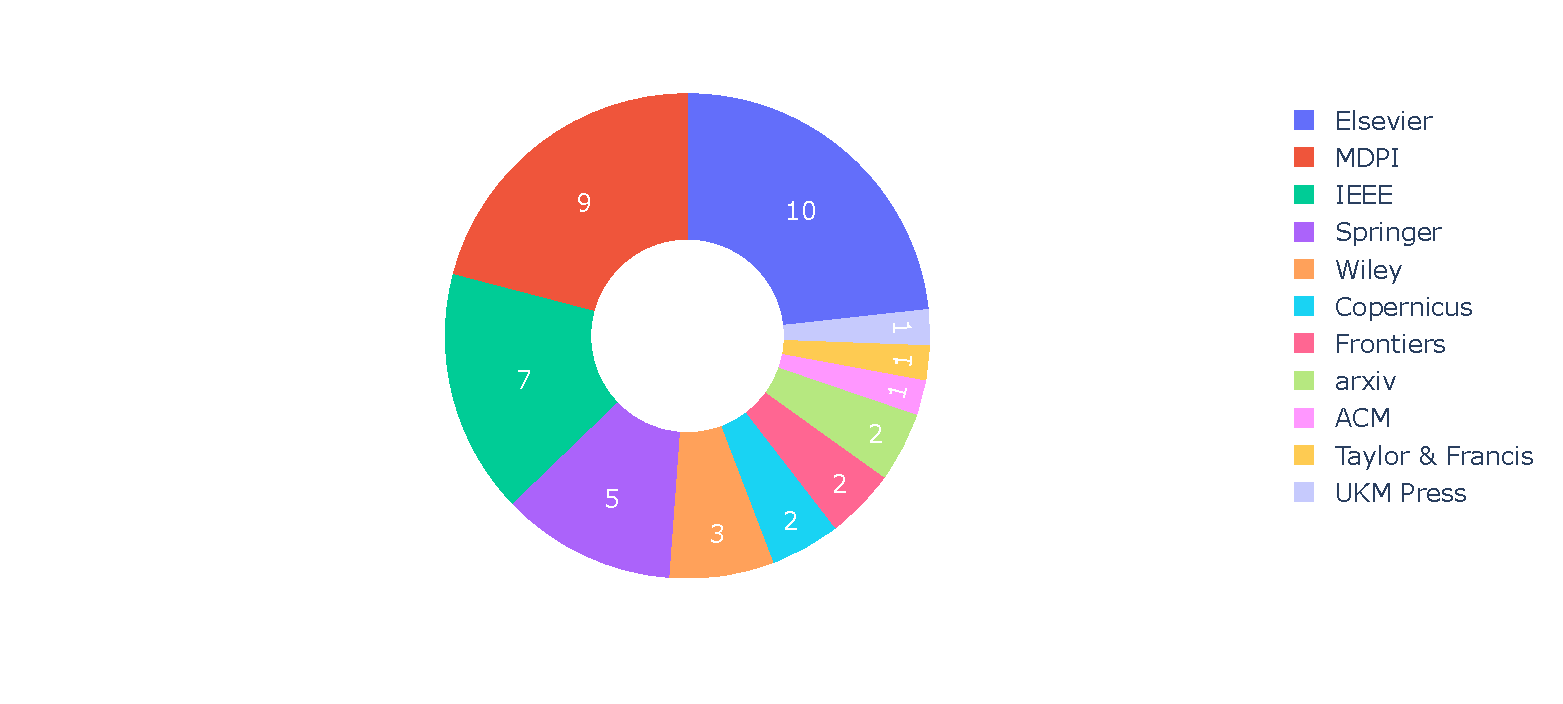
\includegraphics[width=1\textwidth]{Images/ArticuloFuente.pdf}
    \end{center}
    \caption{Fuentes consultadas para la obtención de artículos sobre mapeo de glaciares de montaña en imágenes satelitales mediante aprendizaje automático y aprendizaje profundo.}
    \reference{Elaborado por el autor.}
     \label{fig:ArticuloFuente}
\end{figure}

A diferencia de los datos presentados en el Cuadro~\ref{tab:ResultadoPrimario}, la información aquí se centra en la fuente donde fue indexado el artículo de investigación. Este fue obtenido a través de la consulta al API de Crossref y luego validado manualmente. Se destaca la presencia de fuentes como Elsevier, MDPI e IEEE (ver Figura~\ref{fig:ArticuloFuente}). Dada la naturaleza de la presente revisión sistemática, era previsible encontrar estas fuentes predominantes, ya que son comúnmente citadas en otras revisiones sistemáticas relacionadas a la teledetección. % CITAR

Adicionalmente, se identificó la revista científica en la que se publicó el artículo o la conferencia donde fue presentado. La figura~\ref{fig:ArticuloFuentePublicacion} evidencia que la revista ``Remote Sensing'' de MDPI lidera en número de artículos relacionados con la temática de la presente revisión sistemática. También son notables las publicaciones en revistas afiliadas a la IEEE y ScienceDirect.
 
\begin{figure}[H]
    \begin{center}
    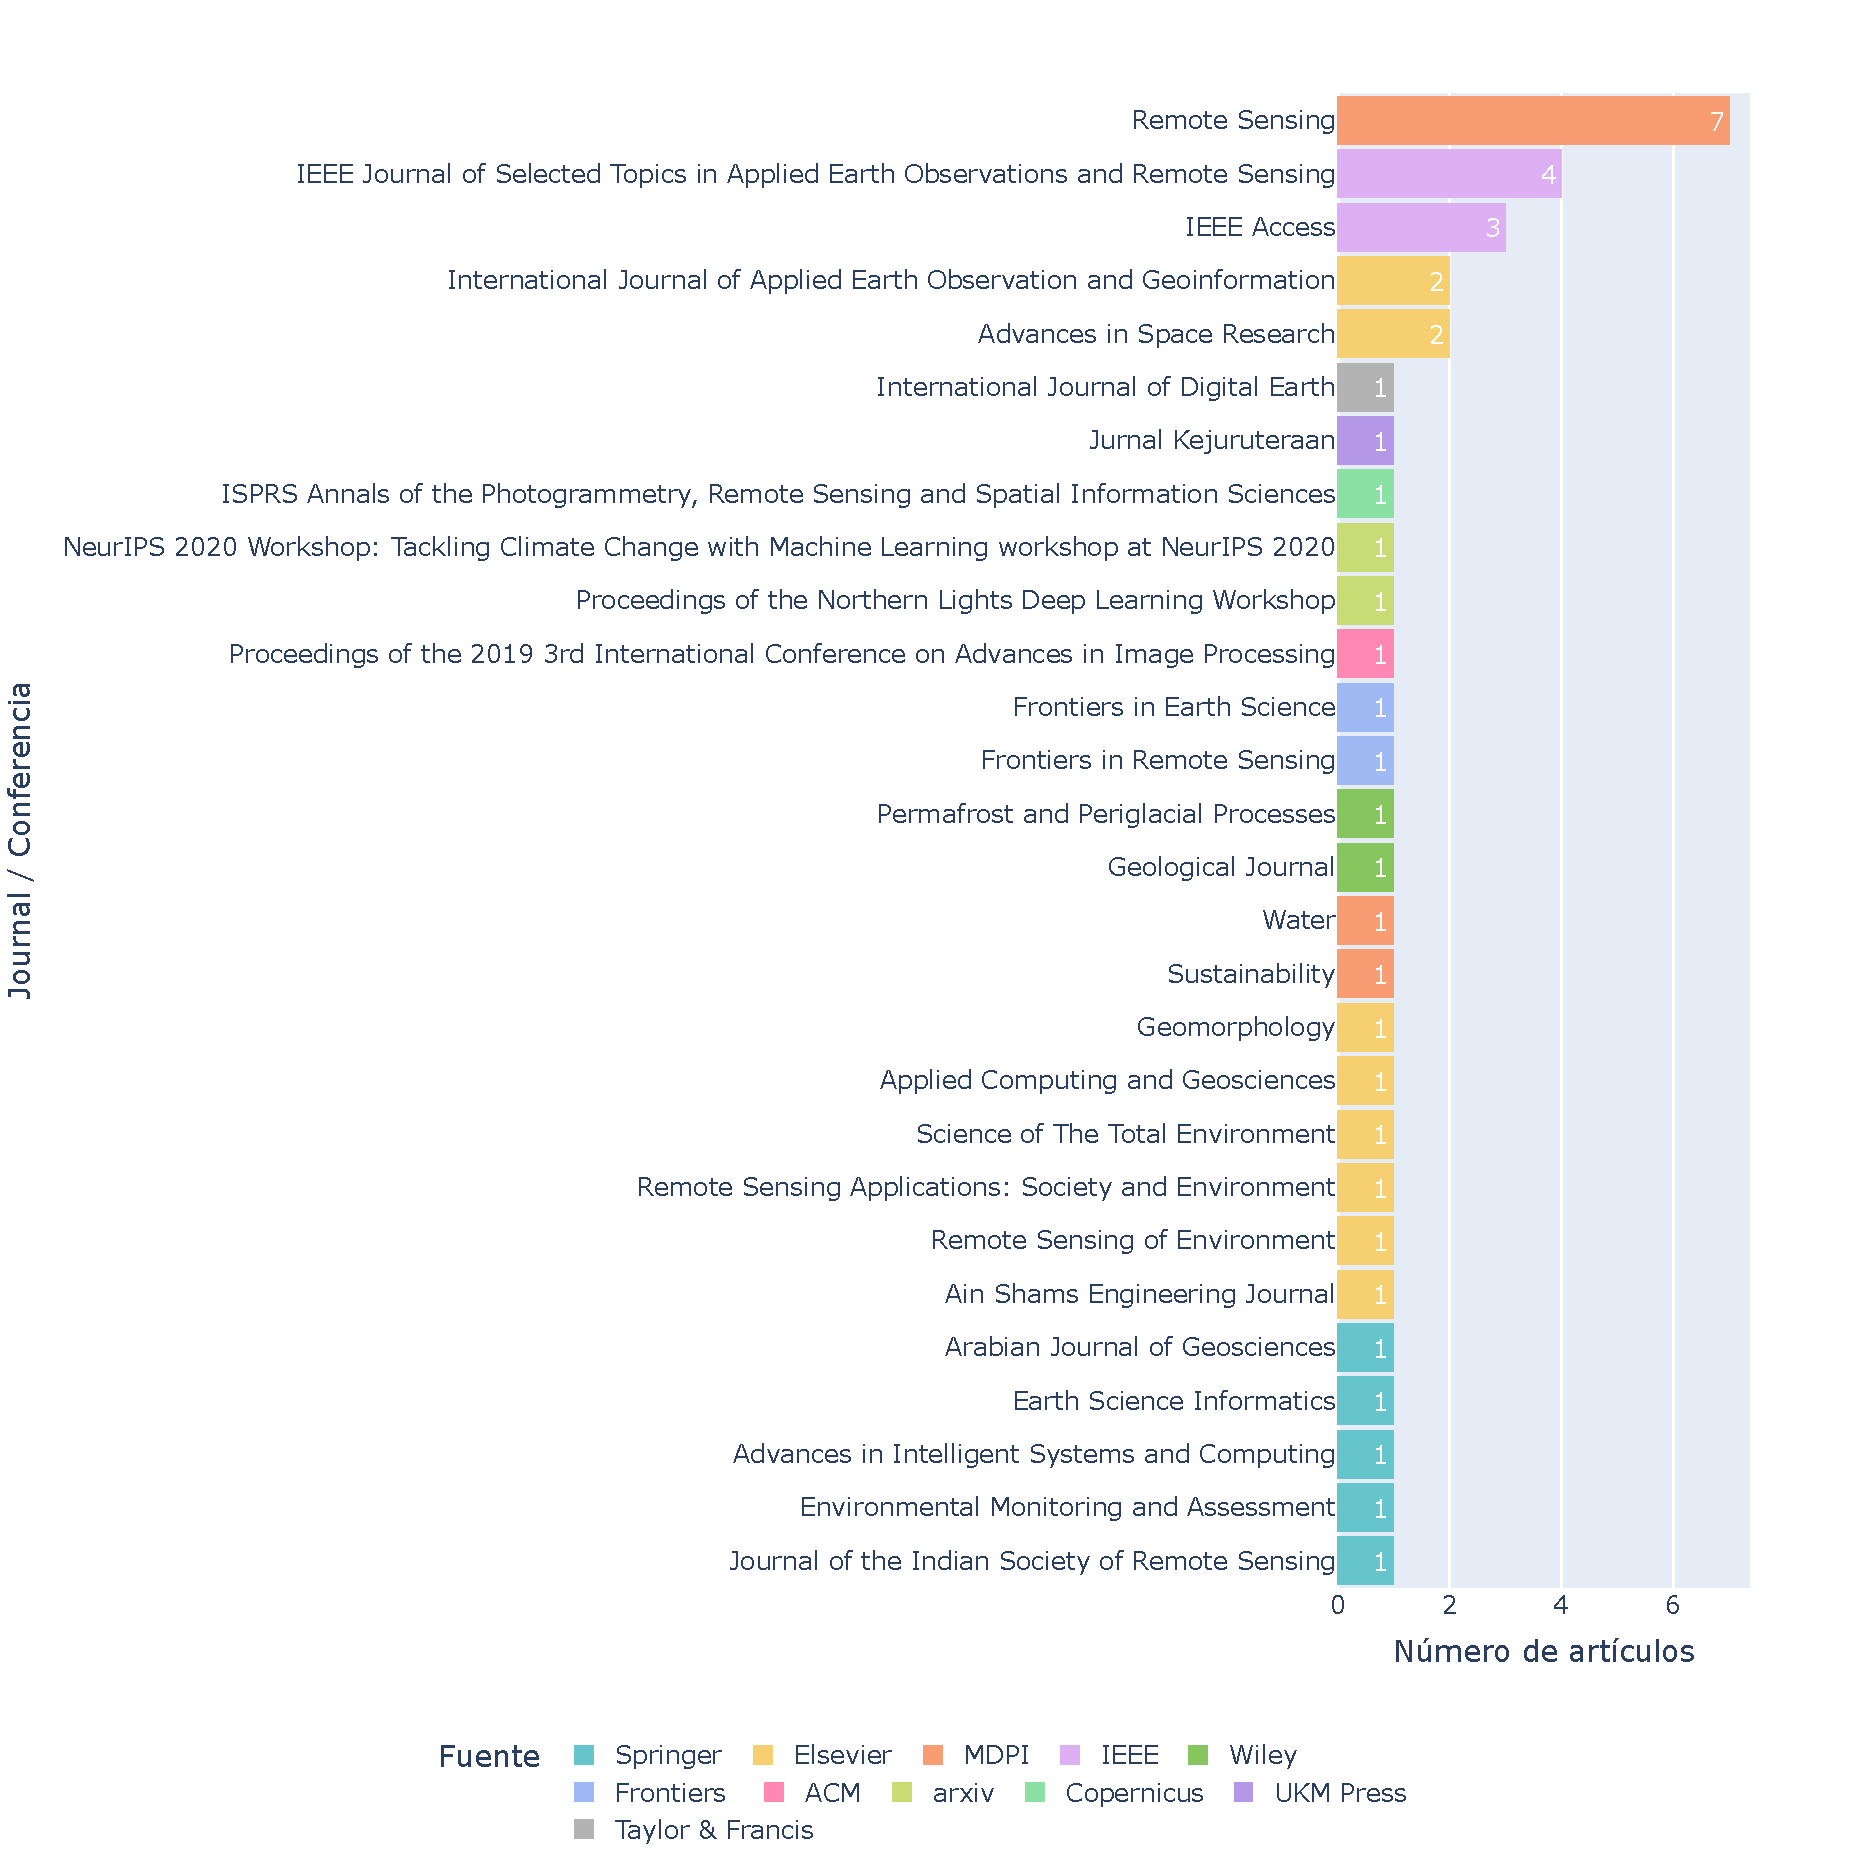
\includegraphics[width=1\textwidth]{Images/ArticuloFuentePublicacion.pdf}
    \end{center}
    \caption{Número de artículos científicos publicados en los últimos años relacionados al mapeo de glaciares usando aprendizaje automático y aprendizaje profundo.}
    \reference{Elaborado por el autor.}
     \label{fig:ArticuloFuentePublicacion}
\end{figure}

\subsubsection{Fase 3: Informe de la revisión sistemática de la literatura}

\textit{Presentación de resultados}

Los resultados de la revisión sistemática se estructuraron en función de respuestas a las preguntas de investigación, descritas en el Cuadro~\ref{tab:PreguntasInvestigacion}. A partir de la información recolectada durante la revisión, se realizó un análisis semi automatizado. Los datos se organizaron en archivos CSV, donde cada fila correspondía a un artículo de investigación y cada columna representaba la información recopilada basada en los criterios establecidos en el Cuadro~\ref{tab:ExtracionDatos}.

\subsubsection{Resultados} 

\textbf{RQ1: ¿Cuáles fueron las técnicas específicas de aprendizaje automático o aprendizaje profundo utilizadas en el mapeo de glaciares?}

El objetivo primordial de esta revisión sistemática consistió en identificar las técnicas contemporáneas empleadas en el mapeo de glaciares en imágenes satelitales, utilizando métodos de aprendizaje automático y aprendizaje profundo.
Se investigó qué algoritmos se aplicaron en cada estudio analizado, con un enfoque particular en los algoritmos basados en redes neuronales convolucionales, ampliamente reconocidos en tareas de visión por computadora y segmentación semántica.
Se observaron propuestas que utilizaban múltiples algoritmos en el proceso de mapeo de glaciares, destacando la alta prevalencia de trabajos que emplearon la arquitectura U-NET o sus modificaciones. Esta observación subraya la relevancia de esta arquitectura en el proceso de mapeo de glaciares utilizando diversas fuentes de imágenes satelitales.





Los algoritmos basados en aprendizaje profundo son los más utilizados en la actualidad para estas tareas dentro del campo de la inteligencia artificial, lo que indica una tendencia consolidada en la metodología de mapeo de glaciares.

\textbf{RQ2: ¿Cuáles fueron las métricas de evaluación empleadas para cuantificar el rendimiento de las técnicas aplicadas en el mapeo de glaciares?}

En la revisión sistemática de la literatura sobre mapeo de glaciares, se observó que una mayoría significativa de estudios recurrió a la métrica de Precisión Global (Overall Accuracy) para evaluar el rendimiento de los métodos empleados.
Además, en los trabajos que implementaron redes neuronales convolucionales específicamente para tareas de segmentación de objetos, se aplicaron métricas más especializadas. Entre ellas, las más destacadas fueron el Índice de Superposición Unión (IoU) y el Índice de Superposición Unión Medio (MIoU), los cuales ofrecen una evaluación más precisa de la segmentación en comparación con la simple precisión global.
Estas métricas reflejan la necesidad de métodos de evaluación versátiles y específicos que puedan adecuarse a las diferentes técnicas y objetivos en el campo del mapeo de glaciares. La elección de métricas apropiadas contribuye a una comparación válida y significativa entre diferentes métodos y aplicaciones.

\textbf{RQ3: ¿Cuáles fueron las principales fuentes de imágenes satelitales utilizadas para realizar el mapeo de glaciares?}

- Hubieron trabajos que emplearon mulktiples fuentes de imagenes sateliales, entro imagenes opticas e imagenes de radar.
- En relaacion a las imagenes opticas, las imagenes derivadas de los satelitales de LandSat fueron las mas utilizadas.
- Asi mismo se hizo una evaluacion de los modelos digitales de elevacion en los estudios que lois utilizaban, dando como resultado una alta presencia ...

\textbf{RQ4: ¿Cómo se construyó el conjunto de datos utilizado para la aplicación de las técnicas de aprendizaje automático o aprendizaje profundo en el mapeo de glaciares?}

En la mayoria de los trabajos se presentaban detallaradmnte los datos utilizadsos, los cuales incluian las imagenes satelitlaes opticas, imagenes satelitales de radas, modelos digitales de elevacion e imagens en alta resilucion cobtenidas generalmente de Google Eath, y generalmente empleadas para tareas de validacion.


\textbf{RQ5: ¿Qué tipos de glaciares se buscaron mapear en el contexto de la investigación?}

- Se destaca la alta presencia de glaciares cubiertos de escombros como los tipos de glaciares que mas se buscaron identificar, estos generalmente deribados de un grupo de .....
- Algunos estudios se enfocaron netamente en la identificacion de glacaires cubiertos de escombros, asi como otros estudios tenenia como objetivo solo el mapeo de glaciares limpios.
- Por otro lado, se identificaron algunos estudios cuyp objetivo final, fue la delimitacion de glaciares, o la delimitación de limites glaciares, pero que empleaban tecnicas de segmentacion de objetivos para posteriormnte realixar el delinado empleadon tecnicas como .....
 
\textbf{RQ6: ¿Cuál fue la región geográfica donde se llevó a cabo el mapeo de glaciares?}
Esto podría deberse a la presencia de una de las cordilleras más importantes del mundo, el Himalaya, y las zonas circundantes con condiciones geográficas similares.

\subsubsection{Discusión}

Algunos paises de europa tambien han publicado estudios. Destaca la poca presencia de estudios relazcinoados a la cordillera de los andes, aunque se han evidenciado estudios en esta region geografoca, estas no generalmente estan enfocados en el mapeo de glaciares, o no se aplican tecnicas basadas en aprendixaje automatico o aprendizaje profundo para su identificacion, lo cual significa una oportudidad para futuros tra

0\subsection{Inventario de glaciares}

\textbf{Inventario de glaciares de Perú}

El Instituto Nacional de Investigación en Glaciares y Ecosistemas de Montaña (INAIGEM) desarrolló el inventario de glaciares de Perú, siendo su última versión oficial publicada en el año 2018. El INAIGEM es el organismo técnico especializado encargado de la investigación científica de los glaciares y ecosistemas de montaña en el Perú.

La metodología propuesta por el INAIGEM para la elaboración del inventario se encuentra detallada en el documento ``Manual Metodológico de Inventario Nacional de Glaciares''. Dicha metodología consta de 8 etapas, que incluyen la recopilación de datos, preprocesamiento, mapeo, caracterización y presentación de resultados, tal como se muestra en la Figura~\ref{fig:MetodologiaInaigem}.

\begin{figure}[H]
    \begin{center}
    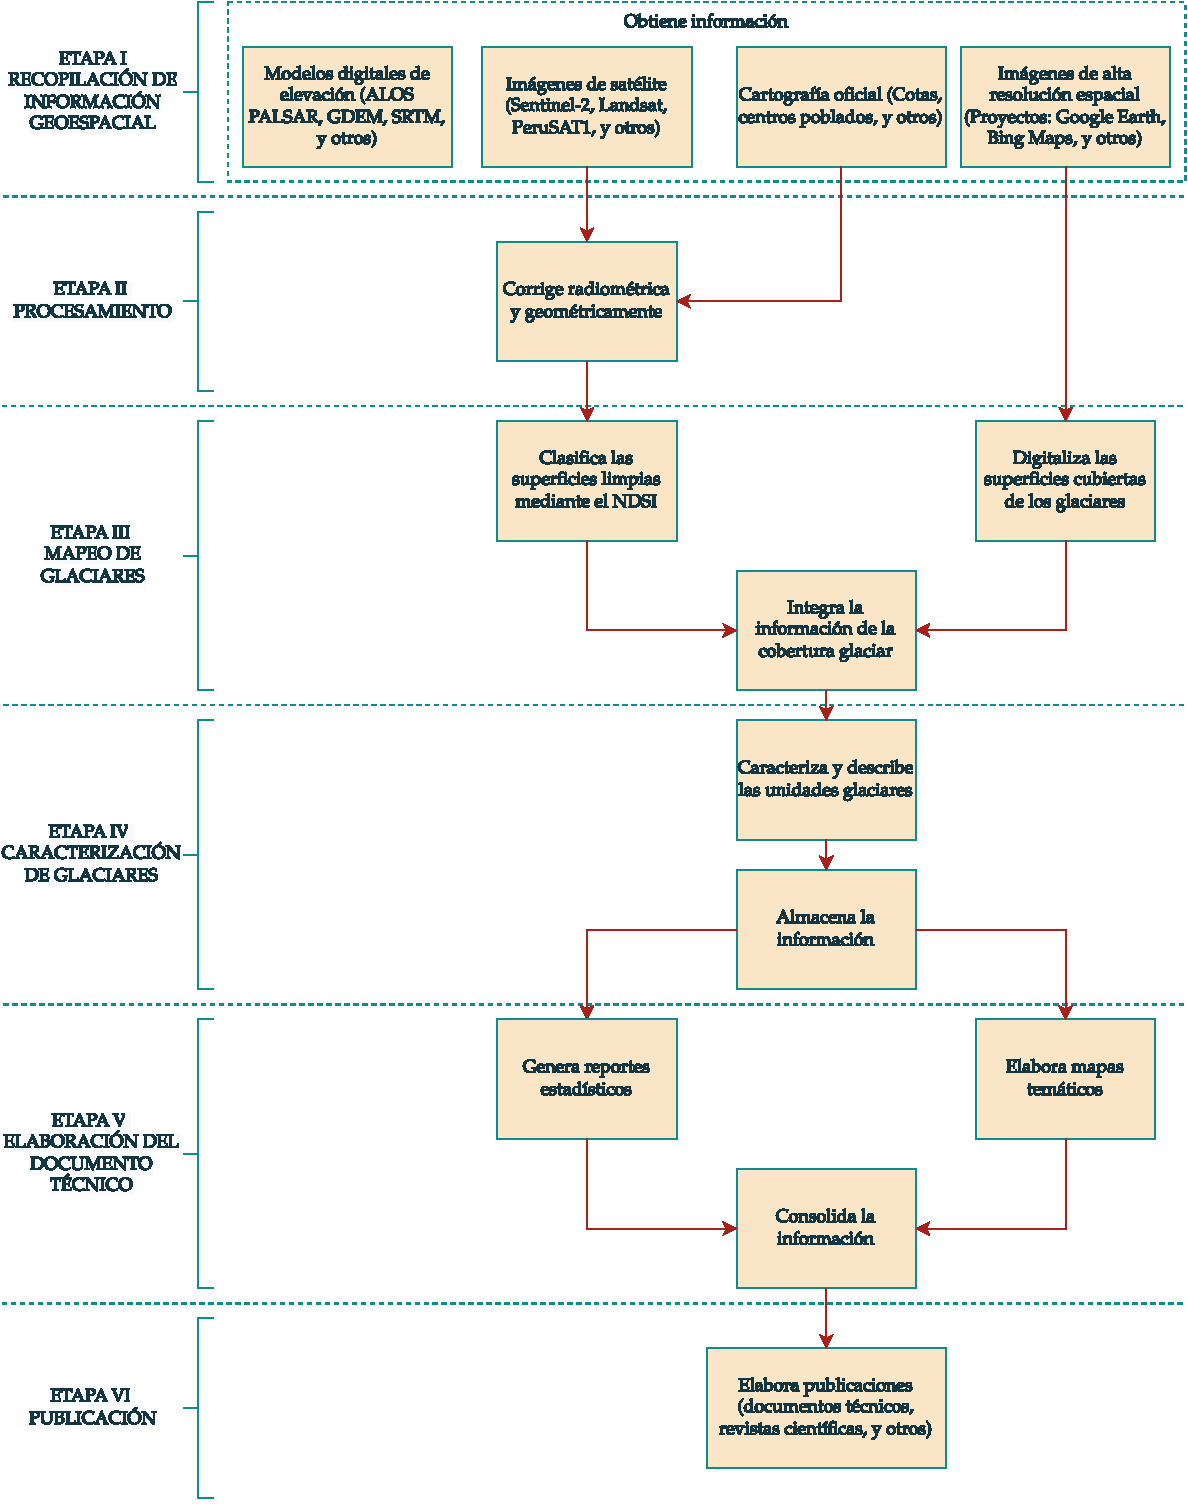
\includegraphics[width=1\textwidth]{Images/MetodologiaInaigem.pdf}
    \end{center}
    \caption{Metodología empleada por el Instituto Nacional de Investigación en Glaciares y Ecosistemas de Montaña para la elaboración del inventario de glaciares de Perú.}
    \reference{Datos tomados de \citeA{inaigem2017manual}.}
     \label{fig:MetodologiaInaigem}
\end{figure}

En la elaboración del inventario se utilizó una variedad de información cartográfica, resaltando sobre todo el uso de imágenes satelitales del Sentinel-2 con resoluciones espaciales de 10 y 20 metros. Las imágenes fueron seleccionadas de acuerdo con la fecha de adquisición (entre los meses de mayo y septiembre), el porcentaje de nubosidad (inferior al 10\%) y la ausencia o escasez de nieve temporal. Además, se recurrió a imágenes complementarias de Aster, Landsat, ResourceSat y RapidEye para realizar análisis multitemporales \cite{inaigem2017manual}.

Durante la elaboración del inventario, se optó por modelos digitales de elevación provenientes del sensor ALOS-PALSAR con una resolución espacial de 12.5 metros. Todos los recursos cartográficos empleados en la construcción del inventario de glaciares están detallados en el Cuadro~\ref{tab:RecursosPeru}.

\begin{table}[H] 
\small
\caption{Información cartográfica utilizada en la elaboración del ``Inventario Nacional de Glaciares del Perú''.\label{tab:RecursosPeru}}
\newcolumntype{C}{>{\centering\arraybackslash}X}
\begin{tabularx}{\textwidth}{Xp{2.8cm}X}
\hline
\textbf{Información} & \textbf{Tipo} & \textbf{Características}.\\ \hline 
Cartas topográficas (Ríos, lagunas, cotas, curvas de nivel y señales). & Vectorial
(base) & Digital (formato
*.cad y *.shp) a
escala 1:25,000 y
1:100,000. \\ \hline 

Limites políticos
(departamento,
provincia y distrito),
centros poblados,
cuencas
hidrográficas, red
vial, límites de áreas
naturales protegidas,
ríos principales y
secundarios. & Vectorial
(base) & Digital a escala
1:100,000. \\ \hline 

Límite de unidades
hidrográficas. & Vectorial
(base) & Digital a escala
1:100,000. \\ \hline 

Cartografía glaciar. & Vectorial/Raster
(base) & Digital a escala
1:100,000 entre los
años 1955 y 1962. \\ \hline

Cartografía glaciar. & Vectorial
(base) & Digital a nivel
nacional a escala
1:100,000 entre los
años 2003 y 2010. \\ \hline

Imágenes de satélite
Landsat, ASTER,
Resourcesat, CBERS y
otros según
requerimiento. & Raster
(material
satelital) & Imágenes de
satélite con varias
bandas para la
evaluación y
análisis
multitemporal. \\ \hline 

Imágenes de satélite
Sentinel-2 o
imágenes
equivalentes. & Raster
(material satelital) & Imágenes con
resolución espacial
entre 10 y 20 m
para el inventario. \\ \hline 

Modelos digitales de
elevación SRTM y
AsterGDEM; en
ambos casos últimas
versiones. & Raster
(material
satelital) & Modelos de
elevación digital
para mejorar o
complementar las
zonas con
anomalías de los
DEM base. \\ \hline

Modelo digital de
elevación (base). & Raster
(material
satelital) & Modelo digital de
elevación con
resolución espacial
de 12.5 m para el
inventario \\ \hline

\end{tabularx}
\reference{Datos tomados de \citeA{inaigem2017manual}.}
\end{table}

En cuanto al software utilizado, se destacan principalmente ArcGIS, ENVI, ERDAS IMAGINE. ArcGIS se empleó para varias tareas, incluyendo la sistematización de cartas topográficas, la delimitación del área de estudio, la obtención de la cobertura glaciar mediante el índice NDSI, la determinación de parámetros y la caracterización de los glaciares, la creación de la base de datos espacial y la elaboración de mapas temáticos. Por otro lado, ENVI y ERDAS IMAGINE se utilizaron para el procesamiento de las imágenes satelitales, la generación de modelos digitales de elevación y sus productos derivados, así como para el análisis multitemporal \cite{inaigem2017manual}.

Los sistemas de coordenadas utilizados en el inventario fueron: WGS 84 / UTM zona 17S, WGS 84 / UTM zona 18S y WGS 84 / UTM zona 19S. Esto se debe a que Perú se encuentra geográficamente ubicado entre estas zonas longitudinales.

La adquisición de los datos se realizo a traves de descarga digital directa de multiples fuentes. 

\textbf{Inventario de glaciares de Chile}

La más reciente versión del Inventario Público de Glaciares en Chile fue publicada en el año 2022. Esta edición fue elaborada por la Unidad de Glaciología y Nieves, perteneciente a la Dirección General de Aguas del Ministerio de Obras Públicas de Chile. En este inventario, se identificaron y clasificaron los glaciares descubiertos, cubiertos y rocosos siguiendo las directrices primarias de la UNESCO, al igual que se hace en otros países de la región. Como detalla \citeA{DGA2022}, la tipología de glaciares abarca desde los situados en montañas hasta los rocosos con cobertura prácticamente completa de rocas. El criterio empleado para su mapeo considera superficies con un área mínima de 1 hectáreas.

Esta versión del inventario representa su primera actualización desde su creación en el año 2014 e incorpora cambios significativos en la metodología y en la tecnología utilizada para el procesamiento de imágenes satelitales. Los polígonos resultantes cuentan con un total de 20 campos alfanuméricos obligatorios, y 21 campos alfanuméricos secundarios, entre los que destacan: el código del glaciar (COD\_GLA), el nombre del glaciar (NOMBRE), la clasificación primaria del glaciar (CLASIFICA), la superficie (ÁREA\_KM2), la fuente de digitalización (FUENTE\_DIG), y otros campos relacionados a la ubicación, morfología y características de los glaciares \cite{DGA2022}.

\begin{table}[H] 
\small
\caption{Imágenes utilizadas en la elaboración del ``Inventario Público de Glaciares de Chile''.\label{tab:ImagenesChile}}
\newcolumntype{C}{>{\centering\arraybackslash}X}
\begin{tabularx}{\textwidth}{p{4.25cm}X}
\hline
\textbf{Imagen} & \textbf{Características}.\\ \hline 
Landsat 8 (OLI) & 15 m de resolución (pansharpened) en combinación R: 7
(infrarrojo de onda corta), G: 5 (infrarrojo cercano), B: 3 (verde).\\ \hline 
Sentinel-2 & 10 m de resolución (multiespectral) en combinación R: 8 (infrarrojo
cercano), G: 4 (rojo), B: 3 (verde).\\ \hline 
Spot 6 & 1.5 m de resolución en color visible.\\ \hline 
Imágenes obtenidas de ``Base Map'' de Arcmap & WorldView-2 y WorldView-4
(0,5 m), WorldView-3 (0,31 m) y GeoEye-1 (0,46 m) en color visible.\\ \hline 
Hycon & Del año 1955 a escala 1:70.000.\\ \hline 
PlanetScope & 3 m de resolución en color visible.\\ \hline 
Ortofotos de vuelos aéreos LiDAR & De los años 2015 y 2019 entre 1 y 1,8 m de
resolución en color visible.\\ \hline  
Google Earth & 1.5 m de resolución en color visible.\\ \hline 
Pléiades & 0.5 m de resolución en color visible.\\ \hline 
RapidEye & 5 m de resolución en color visible.\\ \hline 
\end{tabularx}
\reference{Datos tomados de \citeA{DGA2022}.}
\end{table}

Las imágenes empleadas para el inventario se obtuvieron entre los años 2010 y 2021, principalmente durante las temporadas de fin de verano, cuando la nubosidad era mínima. Se utilizaron imágenes con resoluciones espaciales que varían entre 10 y 3 metros, como se detalla en el Cuadro~\ref{tab:ImagenesChile}. Todos los datos fueron procesados utilizando software especializado, incluyendo LEOWorks 3.0, GlobalMapper 12.0, QGIS 3.4+GRASS y ArcGIS 10.2.1  \cite{DGA2022}.

La clasificación de los glaciares se llevó a cabo siguiendo el esquema propuesto por GLIMS, una estrategia adoptada también por otros países de la región. El mapeo de los glaciares se basó en los hallazgos del inventario de 2014, evidenciando una disminución en la superficie glaciar, pero también identificando nuevas superficies con un tamaño mínimo de 1 hectárea. A su vez, se eliminaron manchas de nieve efímeras que , según ellos, habían sido erróneamente catalogadas como glaciares en la versión anterior. Para el mapeo se utilizaron datos fisiográficos como la pendiente, la altitud media, la altitud mínima, la altitud máxima y la orientación. El sistema de coordenadas empleado fue WGS 84 / UTM zone 19S. Según \citeA{DGA2022}, no se utilizaron técnicas automatizadas, sino que el trabajo fue realizado íntegramente por operadores humanos.

El proceso de validación del inventario de glaciares se realizó a través de una revisión por pares, para la cual se invitó a instituciones, organizaciones y expertos tanto de Chile como del extranjero, con el fin de obtener observaciones y sugerencias. Todas las aportaciones recibidas se incorporaron en la versión final del inventario \cite{DGA2022}.

\textbf{Inventario de glaciares de Argentina}


En Argentina, el ente responsable de la elaboración del inventario y monitoreo del estado de los glaciares y y ecosistemas de montaña es el Instituto Argentino de Nivología, Glaciología y Ciencias Ambientales (IANIGLA) \cite{rojas2020inventario}.

\begin{figure}[H]
    \begin{center}
    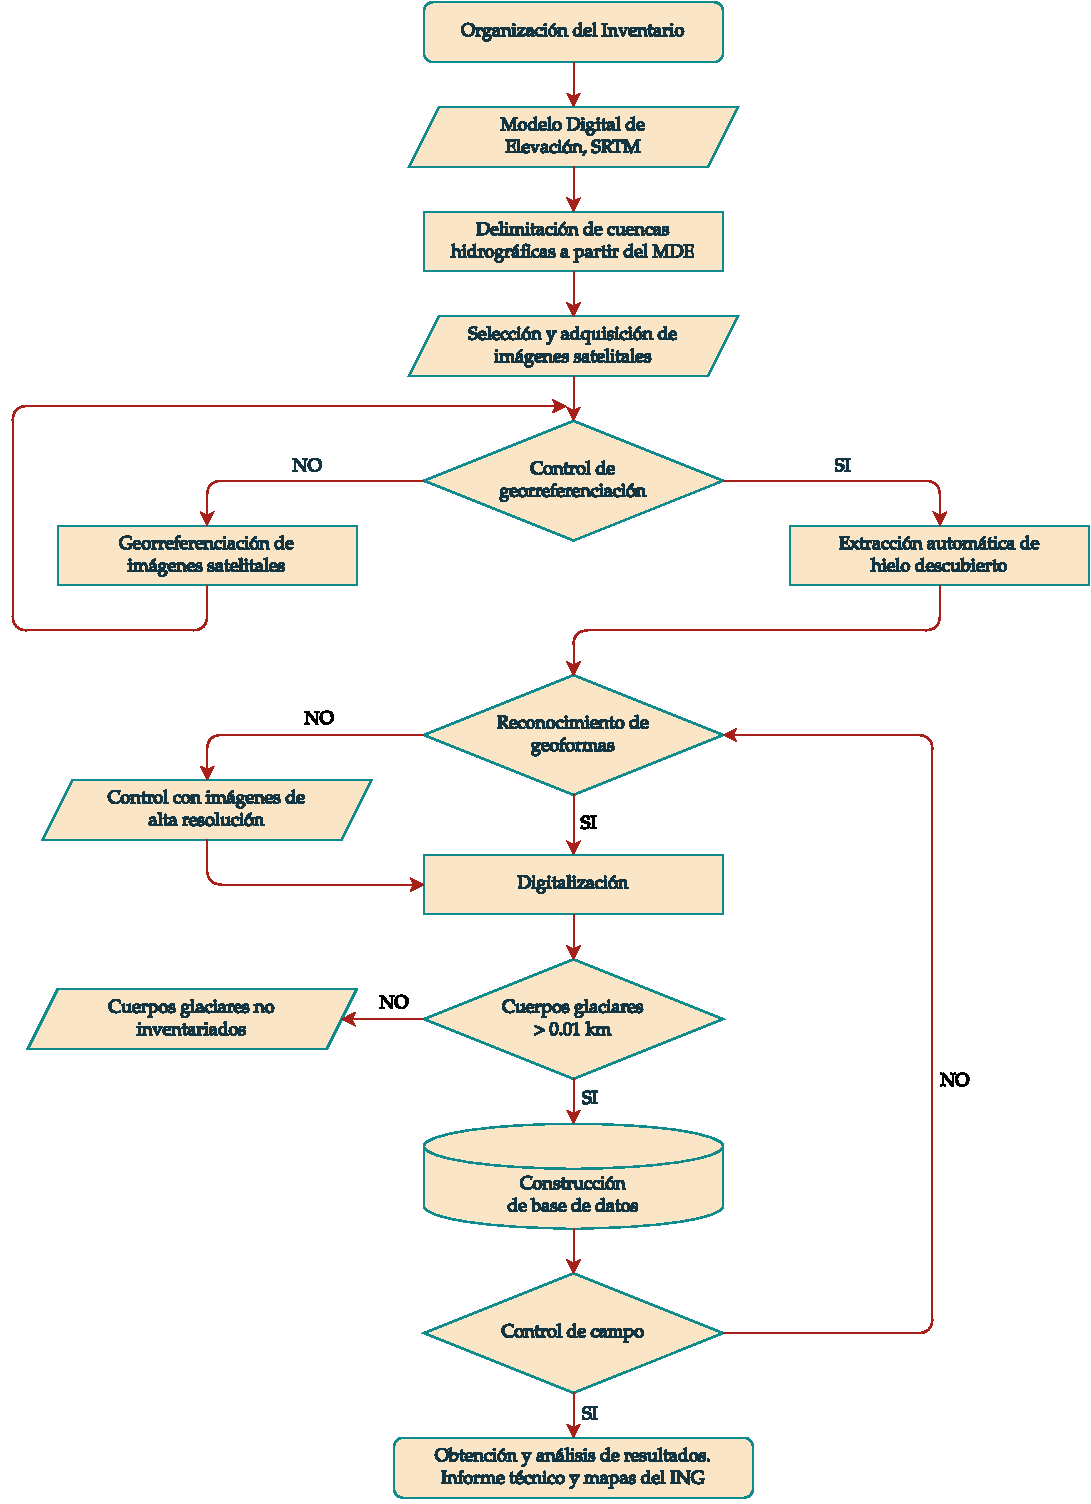
\includegraphics[width=1\textwidth]{Images/MetodologiaIanigla.pdf}
    \end{center}
    \caption{Metodología empleada por el Instituto Argentino de Nivología, Glaciología y Ciencias Ambientales para la elaboración del inventario de glaciares de Argentina.}
    \reference{Datos tomados de \citeA{castro2014manual}.}
    \label{fig:MetodologiaIanigla}
\end{figure}

 

\section{Bases teóricas}

\label{sec:BasesTeoricas}

\subsection{Glaciares}

Los glaciares son estructuras complejas constituidas por hielo, nieve, agua, rocas y sedimentos, que se desplazan bajo la acción de la gravedad y de su propia masa \cite{cuffey2010physics}. Estos se originan en regiones donde la acumulación de nieve supera a la ablación, es decir, la pérdida de masa debido a procesos como la fusión y la sublimación \cite{griggs2002climate}.

En el movimiento de los glaciares intervienen factores internos como la temperatura y la estructura del hielo, y factores externos como la topografía y las condiciones climáticas \cite{benn2010glaciers}. Estos elementos naturales son fundamentales en el balance global del agua dulce y tienen un impacto significativo en el clima y en los ecosistemas \cite{kargel2014global}.

La formación de los glaciares se efectúa mediante la acumulación continua de nieve y hielo en una misma área durante un periodo prolongado, situándose principalmente en regiones de elevada altitud, por encima del nivel de las nieves perpetuas \cite{houghton2001climate}.

\begin{figure}[H]
    \begin{center}
        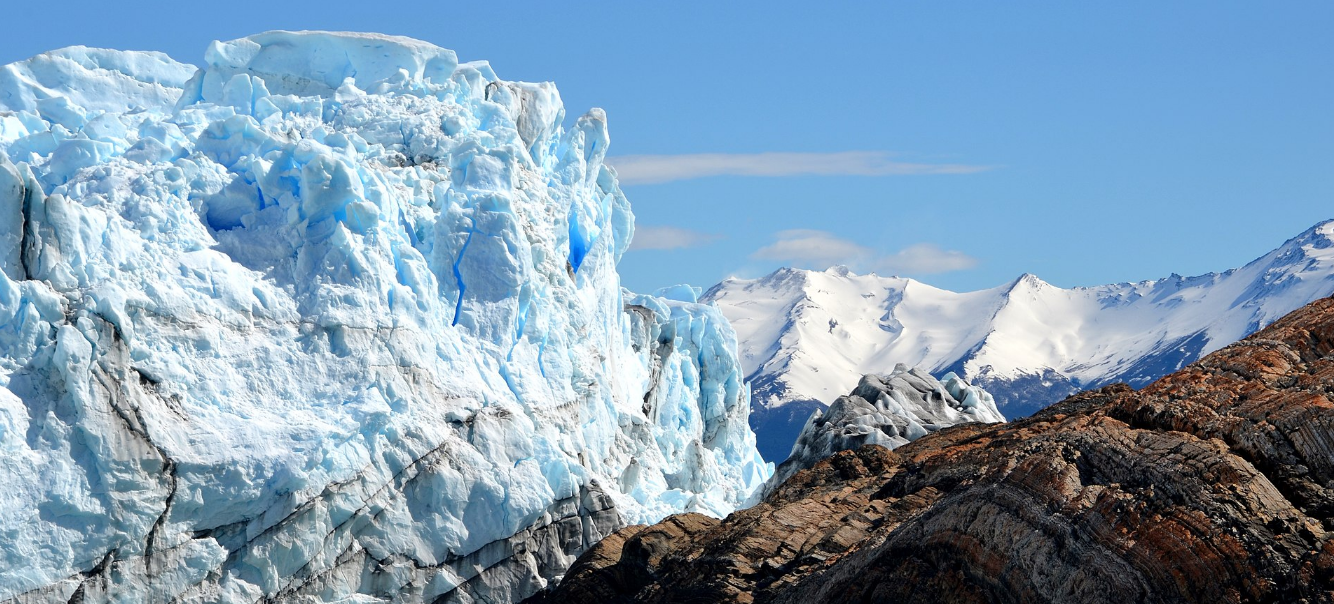
\includegraphics[width=1\textwidth]{Images/GlaciaresFotografia.png}
    \end{center}
    \caption{Fotografía de un glaciar (Glaciar Perito Moreno - Chile)}
    \reference{Datos tomados de \citeA{ermolin2015ambientes}.}
    \label{fig:Glaciar}
\end{figure}

Los glaciares son vitales como reservorios de agua dulce. Según \citeA{ermolin2015ambientes}, sólo el 3\% del agua del planeta es agua dulce. De este porcentaje, el 77\% se halla en la criósfera, región de la corteza terrestre donde predominan las bajas temperaturas y donde el hielo se mantiene durante la mayoría del año \cite{ermolin2015ambientes}. En términos más específicos, el 91\% de las reservas de agua dulce se encuentra en la Antártida, el 8\% en la sabana de Groenlandia y solo el 1\% en los glaciares de montaña continental \cite{benn2010glaciers}. Estos datos subrayan la importancia crítica de la preservación de los glaciares como principales fuentes de agua dulce a nivel global.

\subsubsection{Sistemas glaciares}

Los glaciares se originan debido a la acumulación constante de nieve, proveniente de fenómenos como nevadas, avalanchas, deslizamiento de rocas, por mencionar algunos. Esta acumulación se ve impulsada por condiciones climáticas y topográficas específicas que permiten que la nieve se compacte y forme hielo. Sin embargo, los glaciares no son estáticos; fluyen pendiente abajo impulsados por la fuerza gravitacional de la Tierra. Este movimiento es parte de un delicado equilibrio conocido como balance de masa, que compara las tasas de acumulación y ablación, o pérdida de masa. La ablación puede ocurrir debido a una variedad de factores, como la evaporación y el derretimiento, y se considera que los glaciares están en retroceso cuando la tasa de ablación supera la de acumulación \cite{benn2010glaciers}.

\begin{figure}[H]
    \begin{center}
        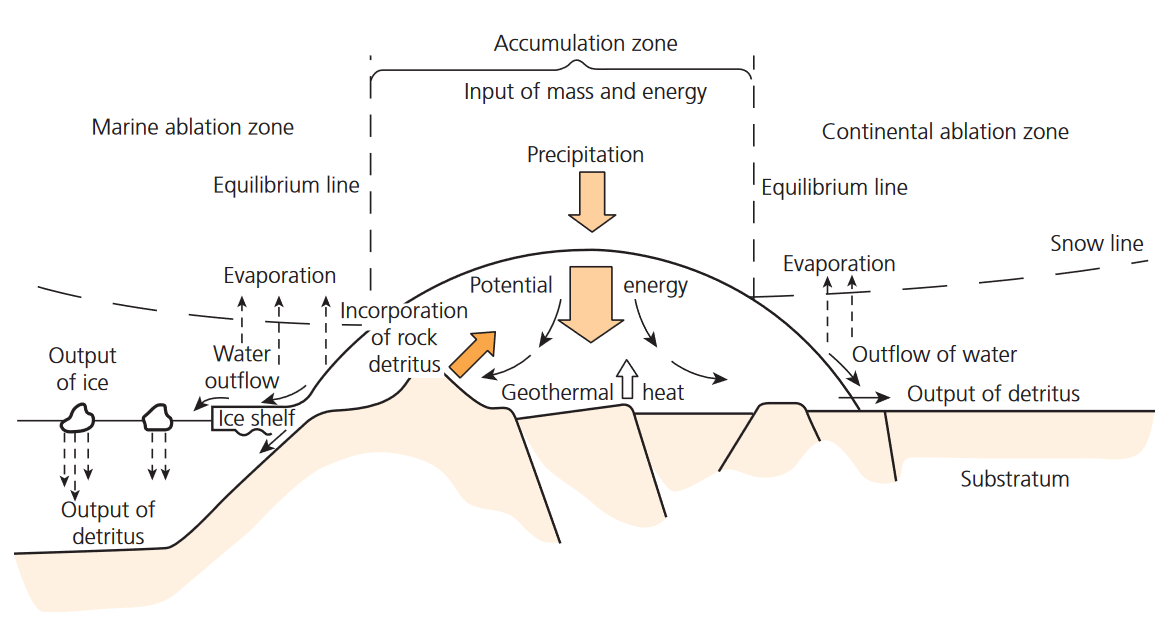
\includegraphics[width=1\textwidth]{Images/Glaciares.png}
    \end{center}
    \caption{Sistemas glaciares}
    \reference{Datos tomados de \citeA{benn2010glaciers}.}
    \label{fig:SistemasGlaciares}
\end{figure}

Factores ambientales como las condiciones atmosféricas y las variaciones térmicas ejercen un impacto directo sobre los glaciares, en particular sobre la altitud de la línea de equilibrio (ELA, por sus siglas en inglés: Equilibrium Line Altitude). La ELA delimita dos regiones diferenciadas en un glaciar: la zona de acumulación y la zona de ablación. En la Figura \ref{fig:SistemasGlaciares}, se observa cómo estas dos zonas se encuentran separadas por la ELA. En la zona de acumulación, la formación de hielo por medio de la acumulación de nieve es predominante sobre el proceso de ablación, es decir, la pérdida de hielo mediante fusión o evaporación. Contrariamente, en la zona de ablación, el proceso de pérdida de hielo es más prominente que el de acumulación  \cite{benn2010glaciers}.

Los glaciares avanzan desde las zonas de acumulación hacia las zonas de ablación a través de deslizamiento y deformación. Este movimiento está regulado por un equilibrio entre las fuerzas que lo impulsan, como la gravedad, y las fuerzas que lo resisten. Cuando están en equilibrio, el flujo del glaciar se mantiene constante \cite{benn2010glaciers, cuffey2010physics}. Sin embargo, factores externos pueden provocar cambios rápidos, como avances o retrocesos. En su trayecto, los glaciares actúan como poderosos agentes erosivos, modelando el paisaje para crear cuencas y fiordos, y eliminando suelo y otros materiales \cite{ermolin2015ambientes}. Además, transportan limo y grava a lo largo de grandes distancias, acumulando estos materiales desde su base hasta el fondo del océano. Dejan un legado de sedimentos y formaciones geográficas, como morrenas y circos, que ofrecen pistas sobre el clima anterior y modifican el terreno, afectando su uso por los seres humanos \cite{benn2010glaciers}.

El agua de deshielo juega un papel esencial, especialmente en la hidrología de las áreas cercanas a los glaciares. Esta agua se incorpora en varios sistemas hídricos, como océanos, ríos y la atmósfera. Participa en un flujo constante entre diferentes reservorios de agua, como océanos, atmósfera, criósfera e hidrosfera, lo que resulta en cambios en el almacenamiento de agua. Por ejemplo, si los glaciares almacenan más agua, el nivel del mar tiende a disminuir y lo contrario ocurre si liberan más agua. Cambios en el volumen del hielo glaciar no solo afectan los niveles del mar, sino también la presión sobre la corteza terrestre y la distribución de la masa global \cite{benn2010glaciers}.

\subsubsection{Partes de un glaciar}

Las partes de un glaciar están estrechamente vinculadas al funcionamiento del sistema glaciar en su conjunto. Según \citeA{inaigem2017manual}, un glaciar se compone de tres partes: la zona de acumulación, la zona de ablación y la altitud de la línea de equilibrio (ELA).

La zona de acumulación corresponde al área donde se acumula la nieve durante un año hidrológico y ofrece datos sobre la cantidad de precipitaciones sólidas en ese periodo. Por otro lado, la zona de ablación es donde predominan los procesos de fusión, evaporación, sublimación y desprendimiento de masas de hielo. La altitud de la línea de equilibrio (ELA) es una línea teórica que separa la zona de acumulación de la zona de ablación \cite{francou2004tropical, benn2010glaciers}.

Como se puede ver en la Figura \ref{fig:PartesGlaciar}, la zona de acumulación y la zona de ablación están separadas por la altitud de la línea de equilibrio (ELA), que representa la zona de equilibrio entre ambas \cite{ideam2012glaciares}.

\begin{figure}[H]
    \begin{center}
        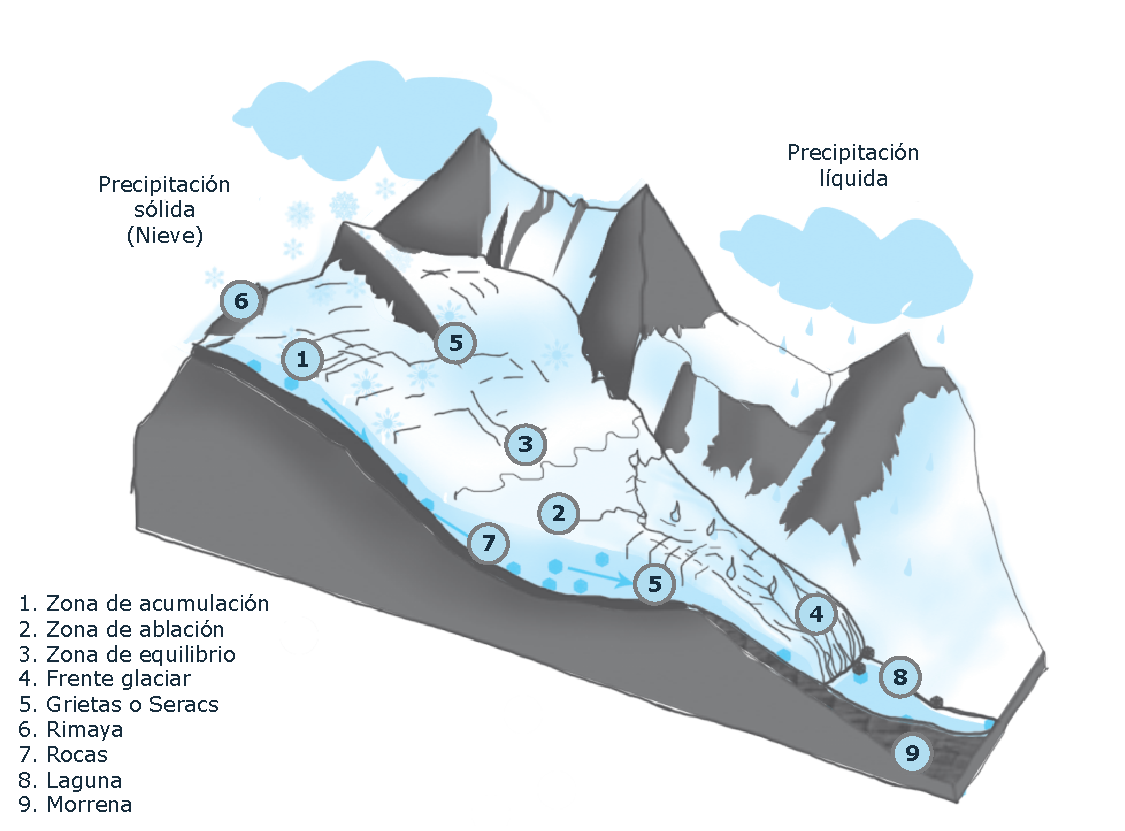
\includegraphics[width=1\textwidth]{Images/PartesGlaciar.pdf}
    \end{center}
    \caption{Partes de un glaciar.}
    \reference{Datos extraídos de \citeA{ideam2012glaciares}.}
    \label{fig:PartesGlaciar}
\end{figure}

En la zona de acumulación, es común encontrar distintos tipos de grietas, como Rimabas y Seracs. Esta área es susceptible a avalanchas debido a las zonas de desprendimiento que pueden extenderse hasta la zona de ablación. Por su parte, la zona de ablación se caracteriza por la presencia de sedimentos y formaciones geográficas como morrenas y circos, así como frentes glaciares, que son aún más propensos a desprendimientos y avalanchas. Además, en esta zona es posible encontrar lagunas de origen glaciar, que son el destino de las aguas de deshielo. Dependiendo de su ubicación, estas aguas pueden dar origen a ríos o desembocar directamente en el mar.

\subsubsection{Clasificación de los glaciares}

La clasificación de los glaciares se determina generalmente por diversos factores, que pueden abarcar la morfología, el tamaño, la dinámica, la temperatura, y el contenido de impurezas en el glaciar. Estas características dan lugar a una amplia clasificación que, según la información recopilada por instituciones especializadas de la región como el Instituto Nacional de Investigación en Glaciares y Ecosistemas de Montaña (Perú) y el Instituto de Hidrología, Meteorología y Estudios Ambientales (Colombia), se detalla en el Cuadro~\ref{tab:ClasificacionGlaciaresI}.

\begin{table}[H]
    \caption{Clasificación de glaciares I}
    \small
    \begin{tabularx}{\linewidth}{@{} *5{X} @{}}
        \hline
        \textbf{Parámetro de clasificación}        & \textbf{Tipo} & \textbf{Descripción}                                                                                                                                                                         \\ \hline
        \multirow{4}{=}{\parbox{4cm}{Morfología}}  & Valle         & Son glaciares que siguen la trayectoria de un valle preexistente, la lengua glaciar es alargada.                                                                                             \\ \cline{2-3}
                                                   & Montaña       & Masas de hielo adheridas a las paredes rocosas, cuyo frente glaciar se encuentra alejada de los valles, distribuida generalmente en pendientes pronunciadas.                                 \\ \cline{2-3}
                                                   & Glaciaretes   & Pequeñas masas de hielo, cuyas zonas de acumulación y ablación no son claramente detectables, este tipo de glaciar generalmente se presenta en glaciares fragmentados.                       \\ \cline{2-3}
                                                   & Capa de hielo & Masa glaciar en forma de domo, cuyo flujo es en forma radial.                                                                                                                                \\ \hline
        \multirow{2}{=}{\parbox{4cm}{Temperatura}} & Templados     & La temperatura del hielo es de 0°C. Existe agua entre la masa de hielo y una probabilidad más alta de deformación. Estos glaciares se desplazan sobre los flujos de agua líquida de la base. \\ \cline{2-3}
                                                   & Fríos         & Glaciares por debajo del punto de fusión, sin agua basal y poco aporte superficial.                                                                                                          \\ \hline
        \multirow{3}{=}{\parbox{4cm}{Dinámica}}    & Activos       & Glaciares con movimiento rápido y evacuación de detritos.                                                                                                                                    \\ \cline{2-3}
                                                   & Pasivos       & Glaciares que fluyen lentamente, lo cual dificulta la evacuación de rocas y la conformación de morrenas. Asociados a masas de hielo en retroceso.                                            \\ \cline{2-3}
                                                   & Estáticos     & Glaciares que no tienen alimentación y presentan lenta fusión del hielo. Pueden considerarse como “relictos sin movimiento”.                                                                 \\ \hline
    \end{tabularx}
    \begin{minipage}{\textwidth}
        \vspace{10pt}
        \reference{Datos tomados de \citeA{ideam2012glaciares}, como se citó en \citeA{inaigem2017manual}}
        \label{tab:ClasificacionGlaciaresI}
    \end{minipage}
\end{table}

\begin{table}[H]
    \caption{Clasificación de glaciares II}
    \small
    \begin{tabularx}{\linewidth}{@{} *5{X} @{}}
        \hline
        \textbf{Parámetro de clasificación}                   & \textbf{Tipo}             & \textbf{Descripción}                                                                                                                                                                                                                                                                                      \\ \hline
        \multirow{3}{=}{\parbox{4cm}{Contenido de impurezas}} & Limpio                    & Glaciares “Blancos” con cobertura superficial característica de nieve y hielo.                                                                                                                                                                                                                            \\ \cline{2-3}
                                                              & Cubiertos                 & Glaciares cubiertos parcial o total por restos adyacentes (detritos y/o fragmentos de rocas) erosionados en su área terminal.                                                                                                                                                                             \\ \cline{2-3}
                                                              & De roca                   & Denominados también glaciares rocosos, presentan una acumulación lenta de restos rocosos (angulares), generalmente con un patrón de cresta / surco distintivo y pendientes empinadas y laterales, cuya longitud es generalmente mayor que su ancho (en forma de lengua) existente en un valle de montaña. \\ \hline
        \multirow{4}{=}{\parbox{4cm}{Localización}}           & Polares                   & Ubicados en latitudes altas o zonas polares.                                                                                                                                                                                                                                                              \\ \cline{2-3}
                                                              & Ecuatoriales / Tropicales & Ubicados cerca de la línea ecuatorial.                                                                                                                                                                                                                                                                    \\ \cline{2-3}
                                                              & Intertropicales internos  & Ubicados entre los trópicos y cercanos a la línea ecuatorial (por ejemplo, Colombia y Ecuador).                                                                                                                                                                                                           \\ \cline{2-3}
                                                              & Intertropicales externos  & Ubicados entre los trópicos y alejados de la línea ecuatorial (por ejemplo, glaciares de Perú y Bolivia).                                                                                                                                                                                                 \\ \hline
    \end{tabularx}
    \begin{minipage}{\textwidth}
        \vspace{10pt}
        \reference{Datos tomados de \citeA{ideam2012glaciares}, como se citó en \citeA{inaigem2017manual}}
        \label{tab:ClasificacionGlaciaresII}
    \end{minipage}
\end{table}
\subsection{Teledetección}

La teledetección, en inglés ``Remote Sensing'', se aplica en una diversidad de campos disciplinarios. Esta tecnología transversal se utiliza en ámbitos como la geología, la meteorología, la ecología, la oceanografía, la agricultura y la planificación urbana, por nombrar algunos \cite{schowengerdt2006remote}.

Dada su aplicación transversal en múltiples disciplinas, la teledetección ha sido objeto de diversas definiciones propuestas por distintos autores. Un ejemplo destacado es el de \citeA{canada2007fundamentals}, quien define a la teledetección como "La ciencia (y hasta cierto punto, arte) de adquirir información sobre la superficie de la Tierra sin estar en contacto directo con ella. Esto se realiza detectando y registrando la energía reflejada o emitida, y procesando, analizando y aplicando dicha información".

Otros autores, como \citeA{chuvieco2016fundamentals}, definen la teledetección como una disciplina centrada en la captura de información sobre objetos terrestres utilizando sensores remotos. Estos instrumentos se encargan de recoger la energía electromagnética, que puede presentarse como radiación reflejada o emitida por la superficie terrestre.

En pocas palabras, la teledetección puede describirse como un campo de estudio basado en la adquisición y procesamiento de información de la superficie terrestre sin la necesidad de estar presente en el lugar estudiado. Su enfoque reside en la interpretación de la radiación electromagnética, un proceso que facilita la observación y recopilación de datos sobre las propiedades y características de la superficie terrestre.

La teledetección tiene como objetivo principal la generación de información relevante para la toma de decisiones o gestión de recursos sobre un determinado fenómeno o área de interés, a partir del procesamiento de la información captada por sensores remotos.

\begin{figure}[H]
    \begin{center}
        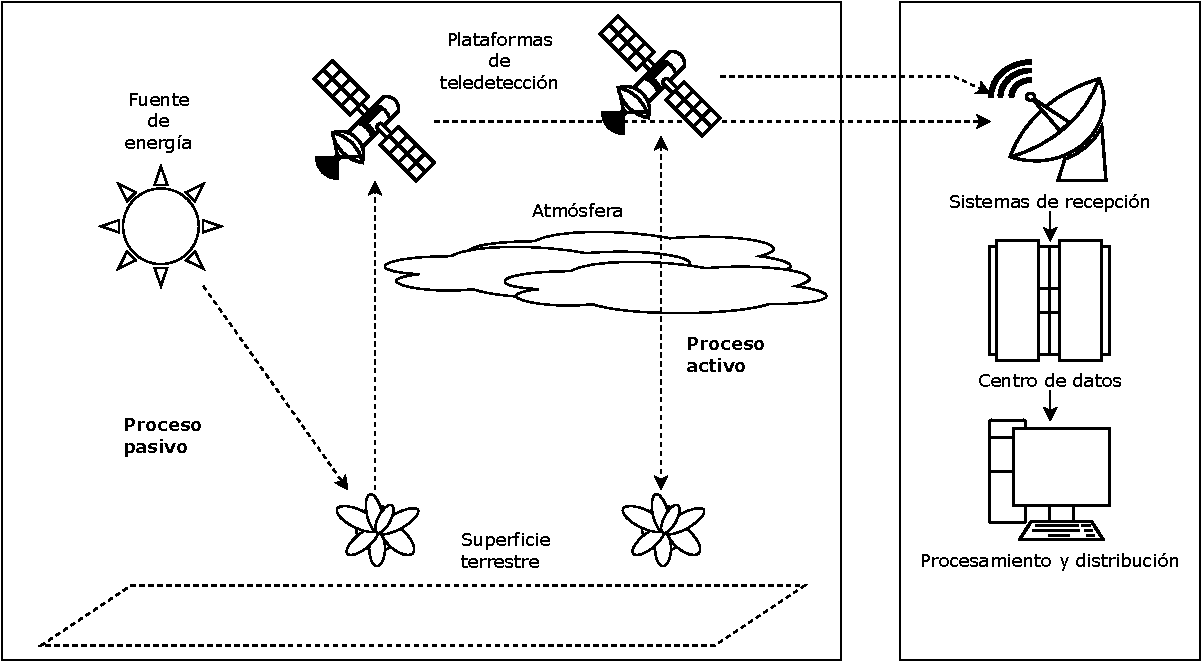
\includegraphics[width=1\textwidth]{Images/Teledeteccion.pdf}
    \end{center}
    \caption{Flujo de la información en un proceso de teledetección.}
    \reference{Elaborado por el autor.}
    \label{fig:Teledeteccion}
\end{figure}

El proceso de teledetección, como se muestra en la Figura~\ref{fig:Teledeteccion}, es un enfoque multidisciplinario que involucra múltiples factores fundamentales para llevar a cabo diversas tareas específicas. Según \citeA{chuvieco2016fundamentals}, este proceso se compone de seis componentes principales:

\begin{enumerate}
    \item \textbf{Fuente de energía}: Este componente se refiere a la fuente que genera la radiación electromagnética que interactúa entre el sensor y la superficie. Principalmente, la fuente más relevante es el Sol, ya que proporciona iluminación y calor a nuestro planeta.
    \item \textbf{Superficie terrestre}: Incluye vegetación, suelos, agua, rocas, nieve, hielo y estructuras humanas. Estas superficies reciben la energía procedente de la fuente y, debido a la interacción física y química con la energía entrante, reflejan y emiten una parte de esa energía de vuelta al sensor satelital. La atmósfera puede filtrar parte o toda la energía, dependiendo de sus concentraciones de gas y partículas.
    \item \textbf{Sensor y plataforma}: El sensor es el dispositivo que mide y registra la energía proveniente de la superficie. La plataforma proporciona los servicios esenciales para el funcionamiento del sensor, como el control de actitud y órbita, suministro de energía y comunicación con el sistema de recepción terrestre. Los satélites son los más comunes en este sentido. Usualmente, un satélite de observación de la Tierra incluye distintos sensores, dependiendo de su misión principal. Los satélites meteorológicos, por ejemplo, suelen tener sensores para detectar humedad atmosférica, temperatura, albedo, ozono o concentraciones de aerosoles.
    \item \textbf{Sistema de recepción en tierra}: Este componente recoge los datos digitales brutos medidos por el sensor, los almacena y los formatea de manera adecuada. El sistema terrestre realiza algunas correcciones de preprocesamiento básicas antes de distribuir las imágenes.
    \item \textbf{Analista}: Es la persona encargada de transformar los datos de la imagen procesada en información temática de interés, utilizando técnicas visuales y/o digitales (en éste último caso, haciendo uso de tecnología especializada, como servidores, dispositivos geodésicos, o estaciones de trabajo).
    \item \textbf{Comunidad de usuarios}: Es el grupo que utiliza la información extraída de los datos originales para una amplia gama de aplicaciones.
\end{enumerate}

\subsubsection{Radiación electromagnética}

Tal como se mencionó anteriormente, para realizar teledetección, es esencial contar con una fuente de energía que ilumine el blanco de estudio, a menos que el propio blanco sea el que emita la energía que se pretende medir. Dicha energía se presenta en forma de radiación electromagnética \cite{canada2007fundamentals}.

Toda materia que posee una temperatura absoluta superior a cero emite energía electromagnética debido a la agitación molecular. La temperatura absoluta se mide convencionalmente en Kelvin ($K$), con incrementos escalados en grados Celsius ($^{\circ}$C). El cero absoluto, que se representa como $0K = -273.15 ^{\circ}C$, es la temperatura más baja alcanzable, en la cual las moléculas cesan completamente su movimiento. Cuando la temperatura de un objeto o sustancia aumenta, las moléculas que lo componen se vuelven más activas y se agitan con mayor intensidad. Esta agitación molecular produce una emisión de energía en forma de radiación electromagnética, la cual puede manifestarse en diversas formas, como luz visible, radiación infrarroja o incluso radiación de alta frecuencia, como los rayos X y los rayos gamma \cite{tempfli2009principles}.

La radiación electromagnética es una forma de energía que se propaga a través de ondas o partículas llamadas fotones. Las propiedades de la radiación electromagnética pueden ser explicadas por dos teorías: La teoría de ondas de la luz y la teoría cuántica \cite{chuvieco2016fundamentals}.

Según la teoría de ondas de la luz, la radiación electromagnética se compone de un campo eléctrico (E) que cambia en su intensidad en una dirección perpendicular al camino que sigue la radiación, y un campo magnético (M) que se ubica en un ángulo de 90 grados respecto al campo eléctrico \cite{canada2007fundamentals}. Ambos campos se desplazan a una velocidad de aproximadamente $c = 3 \times 10^8 \, \mathrm{m/s^{-1}}$ que corresponde a la velocidad de la luz \cite{chuvieco2016fundamentals}.

\begin{figure}[H]
    \begin{center}
        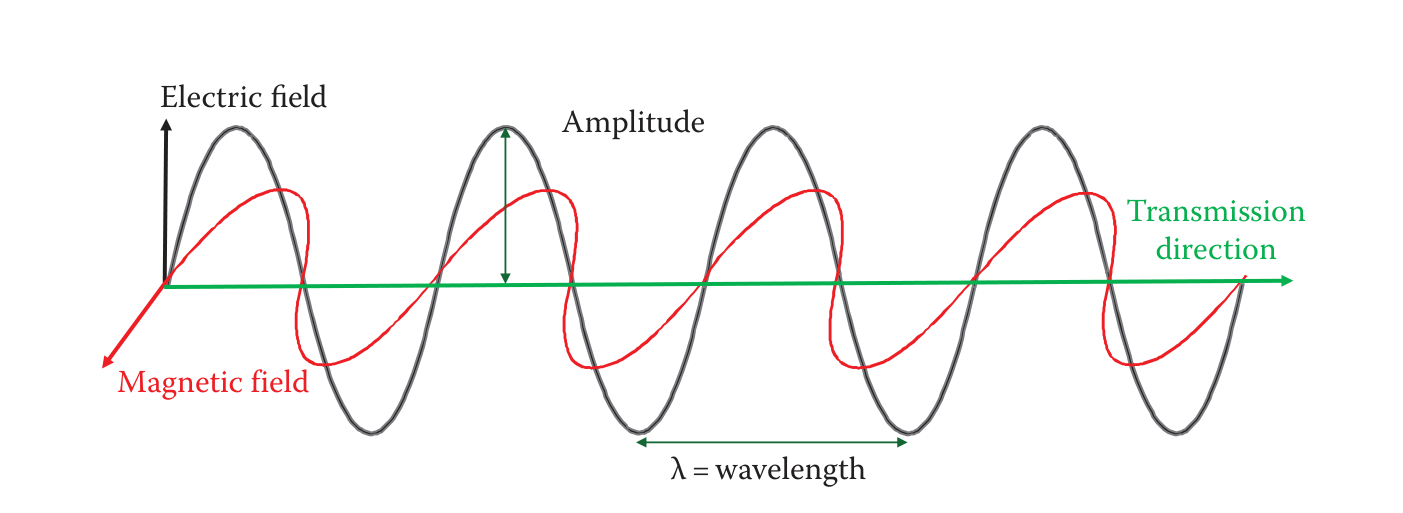
\includegraphics[width=1\textwidth]{Images/ComponentesRadiacionElectromagnetica.png}
    \end{center}
    \caption{Propagación de la radiación electromagnética y sus componentes eléctricos y magnéticos oscilantes.}
    \reference{Datos tomados de \citeA{chuvieco2016fundamentals}.}
    \label{fig:ComponentesRadiacionElectromagnetica}
\end{figure}

Como se muestra en la Figura~\ref{fig:ComponentesRadiacionElectromagnetica}, la radiación electromagnética oscila en un dirección específica. Estas ondas pueden ser descritas en función de su longitud (\(\lambda\)) y su frecuencia (\(\nu\)), las cuales están relacionadas por:

\begin{equation}
    \label{eq:LongitudOndaFrecuencia}
    c = \lambda \times \nu
\end{equation}

donde:
\begin{itemize}
    \item $c$ es la velocidad de la luz $(3 \times 10^8 \, \mathrm{m/s^{-1}})$.
    \item \(\lambda\) es la longitud de onda o la distancia entre dos picos sucesivos (generalmente en micrómetros, 1 $\mu$m = \(10^{-6}\) m; o nanómetros, 1 $n$m = \(10^{-9}\) m).
    \item \(\nu\) es la frecuencia, o el número de ciclos que pasan por un punto fijo por unidad de tiempo (en hercios, ciclos $s^{-1}$).
\end{itemize}

Por otro lado, según la teoría cuántica de la luz, la radiación se describe como una secuencia de paquetes de energía discretos conocidos como fotones o cuantos, los cuales tienen una masa igual a cero. La cantidad de energía transportada por un fotón es directamente proporcional a su frecuencia:

\begin{equation}
    \label{eq:TeoriaCuanticaLuz}
    E = h \times \nu
\end{equation}

donde:
\begin{itemize}
    \item $E$ es la energía radiante de un fotón (en joules, $J$).
    \item \(\nu\) es la frecuencia.
    \item $h$ es la constante de Planck (\(6.626 \times 10^{-34} \, \mathrm{J \, s}\)).
\end{itemize}

La ecuación de la energía de un fotón en términos de la velocidad de la luz y la longitud de onda de la onda electromagnética se expresa como:

\begin{equation}
    E = \frac{{h \times c}} {{\lambda}}
\end{equation}

donde:

\begin{itemize}
    \item $E$ es la energía radiante de un fotón (en joules, $J$).
    \item $c$ es la velocidad de la luz $(3 \times 10^8 \, \mathrm{m/s^{-1}})$.
    \item $h$ es la constante de Planck (\(6.626 \times 10^{-34} \, \mathrm{J \, s}\)).
    \item \(\lambda\) es la longitud de onda o la distancia entre dos picos sucesivos (generalmente en micrómetros, 1 $\mu$m = \(10^{-6}\) m; o nanómetros, 1 $n$m = \(10^{-9}\) m).
\end{itemize}

Por lo tanto, existe una relación inversa entre la longitud de onda y la frecuencia de una radiación. A medida que la longitud de onda aumenta o la frecuencia disminuye, el contenido de energía también disminuye (ver Figura~\ref{fig:RelacionLongitudOnda}). Esto implica que la detección de radiaciones de longitud de onda larga se vuelve más difícil en comparación con las de longitud de onda corta, ya que las primeras tienen menos energía y requieren métodos de detección más sensibles \cite{chuvieco2016fundamentals}

\begin{figure}[H]
    \begin{center}
        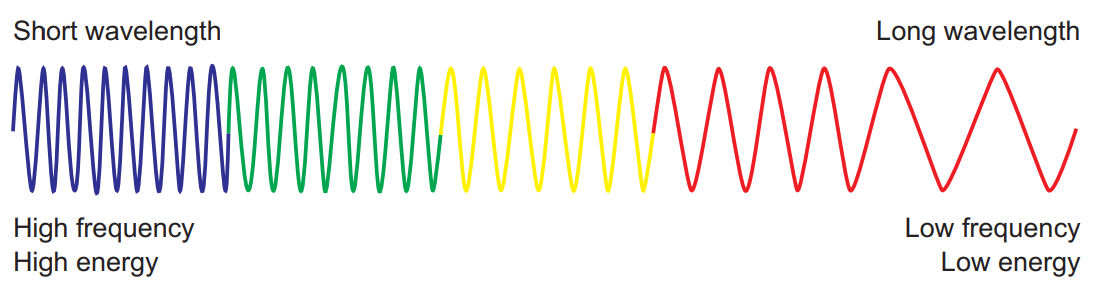
\includegraphics[width=1\textwidth]{Images/RelacionLongitudOnda.png}
    \end{center}
    \caption{Relación inversa entre la longitud de onda y la frecuencia.}
    \reference{Datos tomados de \citeA{tempfli2009principles}.}
    \label{fig:RelacionLongitudOnda}
\end{figure}

Las radiaciones de mayor energía y menor longitud de onda son los rayos gamma y los rayos X, utilizados en aplicaciones médicas y observación astronómica, mientras que las radiaciones de menor energía y mayor longitud de onda se utilizan en las telecomunicaciones, radio y televisión \cite{chuvieco2016fundamentals}. Estas diferentes formas de radiación se distribuyen a través de un amplio rango de frecuencias y longitudes de onda, conocido como espectro electromagnético.

\subsubsection{Espectro electromagnético}

El espectro electromagnético es la distribución de energías de las radiaciones electromagnéticas, se extiende desde los rayos gamma, que son de longitud de onda extremadamente corta $10^-11 m$, hasta las ondas de radio de gran longitud $10^5m$ \cite{joseph2005fundamentals}.

\begin{figure}[H]
    \begin{center}
        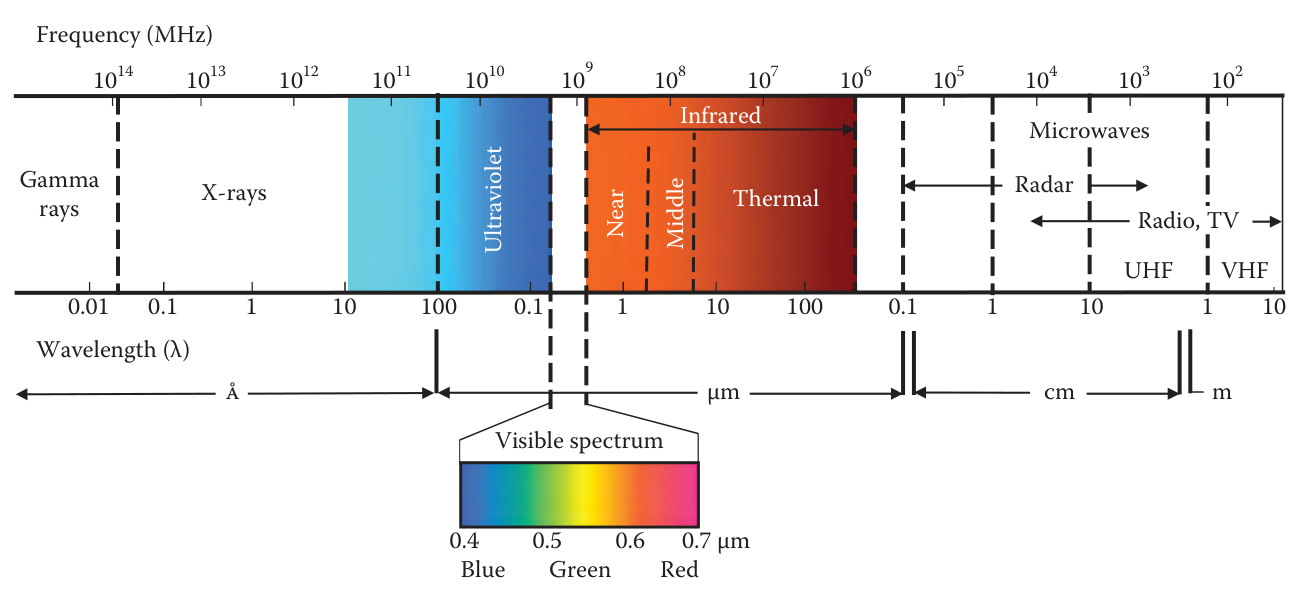
\includegraphics[width=1\textwidth]{Images/EspectroElectromagnetico.png}
    \end{center}
    \caption{Espectro electromagnético.}
    \reference{Datos tomados de \citeA{chuvieco2016fundamentals}.}
    \label{fig:EspectroElectromagnetico}
\end{figure}

La Figura~\ref{fig:EspectroElectromagnetico} muestra el espectro electromagnético, que está dividido en diversas regiones, cada una denotando un comportamiento distinto de las ondas electromagnéticas durante los procesos de emisión, transmisión y absorción.

En el espectro electromagnético, la región de los rayos gamma es caracterizada por ondas con frecuencias que suelen ser mayores a $10^{19}$ Hz, y longitudes de onda menores a $10^{-11}$  \cite{chuvieco2016fundamentals}. Dicha región alberga una gran cantidad de energía, lo suficiente para alterar la estructura de los átomos y moléculas. Esta capacidad puede generar mutaciones genéticas y condiciones carcinógenas en organismos vivos. Los rayos gamma, debido a su elevada energía y capacidad de penetración, son una considerable amenaza para la salud y la seguridad.

Posteriormente en el espectro, los rayos X se sitúan con frecuencias generalmente en el rango de $10^{16}$ Hz a $10^{19}$ Hz, y longitudes de onda entre $10^{-8}$ m y $10^{-11}$ m. Los rayos X son ampliamente utilizados en la medicina debido a su capacidad para atravesar los tejidos del cuerpo humano, lo que permite obtener imágenes de alta resolución de las estructuras internas para diagnósticos y tratamientos médicos.

En el extremo opuesto del espectro electromagnético se ubican las ondas con frecuencias más bajas, y longitudes de onda más largas. Esta sección del espectro es vital para las telecomunicaciones, ya que estas ondas pueden recorrer grandes distancias con mínima pérdida de energía y tienen la capacidad de difractarse alrededor de obstáculos. Estas características hacen que estas ondas sean ideales para la transmisión de información a larga distancia, encontrando uso en servicios como la radiodifusión, la televisión y la telefonía móvil.

En cuanto a las regiones del espectro electromagnético que son utilizadas para tareas de teledetección, generalmente se emplean las áreas desde el ultravioleta hasta las microondas \cite{chuvieco2016fundamentals}. Cada una de estas regiones, y las intermedias, ofrece a la teledetección una serie de capacidades únicas debido a las diferentes características de las ondas electromagnéticas que se encuentran en cada una. Las diferencias en frecuencia, longitud de onda y energía entre las distintas regiones del espectro, resultan en variaciones en la forma en que estas ondas interactúan con la atmósfera y con la superficie terrestre, proporcionando una diversidad de información en la teledetección.

Las regiones del espectro electromagnético que se emplean en teledetección son:

\begin{itemize}

    \item \textit{Región Ultravioleta (UV)}: Justo antes del espectro visible, presenta longitudes de onda más breves que la luz visible y más largas que los rayos X. Esta se ubica después del segmento violeta del espectro visible, de ahí su denominación. La radiación UV, mayormente absorbida por la atmósfera terrestre, cuando es detectada, puede brindar datos significativos para investigar la atmósfera, la capa de ozono y los efectos biológicos de la radiación solar. Ciertos materiales en la superficie terrestre, principalmente piedras y minerales, emiten luz visible al estar expuestos a radiación UV, fenómeno denominado fluorescencia, lo que facilita su identificación y estudio \cite{canada2007fundamentals}.

    \item \textit{Región del Espectro Visible (VIS)}: Engloba las longitudes de onda que el ojo humano puede captar y donde la energía solar es más intensa \cite{chuvieco2016fundamentals}. El espectro visible se puede descomponer en tres colores fundamentales: azul (0.4-0.5 µm), verde (0.5-0.6 µm) y rojo (0.6-0.7 µm) \cite{canada2007fundamentals}. Esta región visible es particularmente útil para examinar fenómenos como la vegetación, la transparencia del agua y la composición del suelo.

    \item \textit{Región del Infrarrojo Cercano (NIR)}: Esta región se localiza justo fuera del límite de percepción humana y se la conoce como infrarrojo reflectante o fotográfico. Una sección de esta región espectral (0.7-0.9 $\mu m$) puede ser detectada usando películas especiales. El NIR es relevante por su sensibilidad para determinar el estado de salud de las plantas y la humedad del suelo \cite{tempfli2009principles,emery2017introduction}.

    \item \textit{Región del Infrarrojo Medio (MIR)}: Esta región espectral se ubica entre las regiones NIR y TIR.

          \begin{enumerate}
              \item De 1.2 a 2.5 µm, la influencia de la energía solar es aún muy notable, comúnmente conocida como la región SWIR \cite{tempfli2009principles}. Esta región proporciona las mejores estimaciones de la humedad, contenido de suelo y vegetación \cite{chuvieco2016fundamentals}.
              \item De 3 a 8 µm, la señal se vuelve una mezcla de energía solar reflejada y energía emitida por la superficie, siendo el componente emitido más destacado conforme las longitudes de onda se expanden. \item El intervalo de 3-5 µm es especialmente útil para detectar fuentes de alta temperatura, como volcanes o incendios \cite{chuvieco2016fundamentals}.
          \end{enumerate}

    \item \textit{La región del Infrarrojo Térmico (TIR)}: Abarca la energía emitida por la superficie terrestre y se emplea para mapear las temperaturas superficiales, detectar la evapotranspiración de la vegetación, analizar propiedades de hielos y nubes, estudiar el impacto del calor urbano y distinguir tipos de rocas \cite{canada2007fundamentals,emery2017introduction}.

    \item \textit{Región de las Microondas (MW)}: En esta región espectral operan los sistemas de radar de imágenes. Su ventaja principal es la baja absorción atmosférica, características por el cual, se puede obtener información a través de las nubes. La radiación de microondas también puede penetrar las copas de los bosques hasta varias profundidades y son muy útiles para discriminar vegetación, cobertura de nieve, rugosidad superficial, dirección de las olas o la forma y orientación de los hidrómetros atmosféricos \cite{emery2017introduction}.

\end{itemize}

Cada una de estas regiones del espectro electromagnético presenta características y ventajas únicas para la teledetección, permitiendo la recopilación de datos que pueden ser empleados en una variedad de aplicaciones.

\subsubsection{Interacción de la radiación electromagnética con la atmósfera}

El sol, siendo una de las fuentes primordiales de energía electromagnética, juega un papel crucial en el sustento de la vida en la Tierra. No obstante, para que su radiación llegue a la superficie terrestre, es necesario que atraviese una considerable extensión de la atmósfera \cite{tempfli2009principles}.

La constitución de la atmósfera es sumamente diversa, incluyendo gases tales como nitrógeno ($N$, representando el 78\% de la atmósfera), oxígeno ($O_{2}$, con un 21\%), argón ($Ar$, alrededor del 0.9\%), vapor de agua ($H_{2}O$, aproximadamente 0.04\%), dióxido de carbono ($CO_{2}$, alrededor del 0.033\%) y ozono ($O_{3}$, un 0.012\%). No solo se componen de gases, también existen partículas sólidas en suspensión, denominadas aerosoles, que interactúan activamente con la radiación electromagnética. Estos aerosoles abarcan una variedad de sustancias, desde sal oceánica hasta partículas de polvo, carbono y residuos de combustión \cite{chuvieco2016fundamentals}.

\begin{figure}[H]
    \begin{center}
        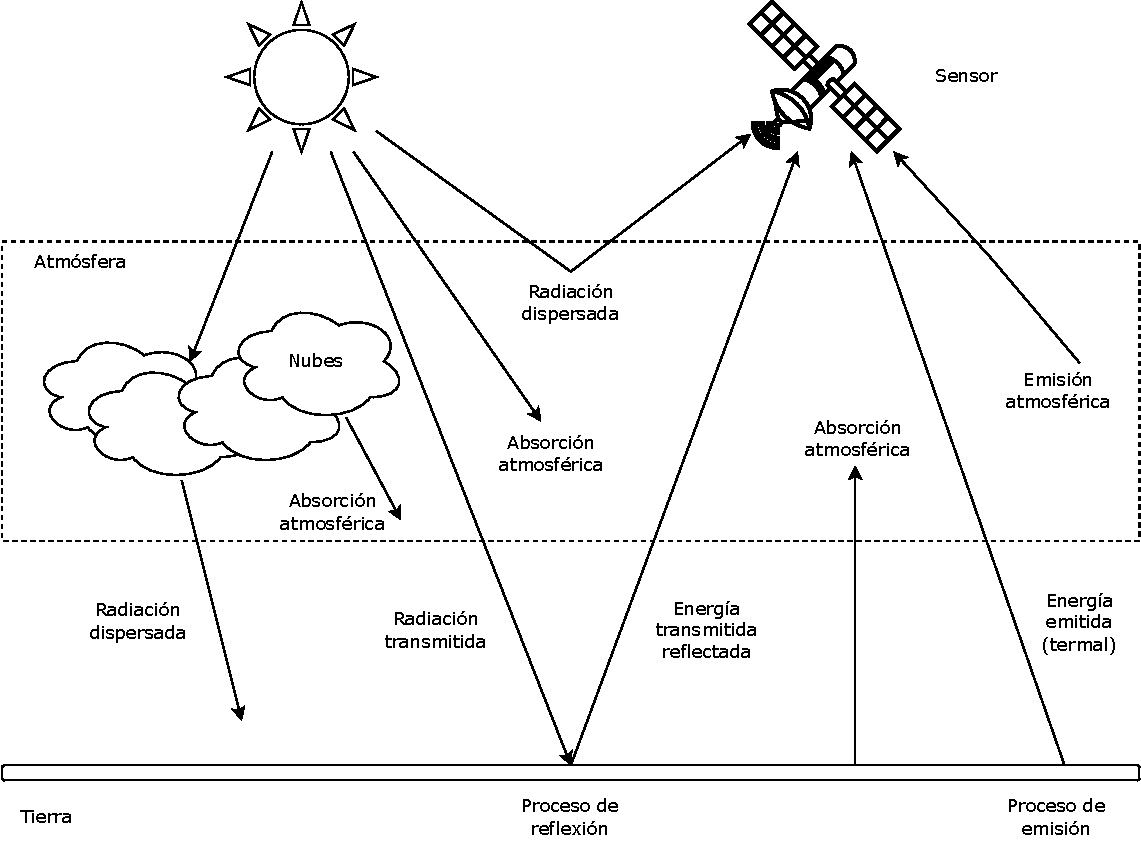
\includegraphics[width=1\textwidth]{Images/InteraccionAtmosfera.pdf}
    \end{center}
    \caption{Ventanas atmosféricas vistas a través del porcentaje de transmisión atmosférica.}
    \reference{Datos tomados de \citeA{tempfli2009principles}.}
    \label{fig:InteraccionAtmosfera}
\end{figure}

Los efectos de estos elementos atmosféricos pueden clasificarse en tres categorías distintas: Absorción, Dispersión, y Emisión \cite{chuvieco2016fundamentals}, tal y como se puede ver en la Figura~\ref{fig:InteraccionAtmosfera}.

\textbf{a) Absorción y transmisión atmosférica}

El fenómeno de absorción actúa como un filtro selectivo, ya que las moléculas presentes en la atmósfera absorben energía en diferentes longitudes de onda. Algunas de las causas de esta filtración son los componentes atmosféricos como el oxígeno atómico, el ozono, el vapor de agua y el dióxido de carbono \cite{chuvieco2016fundamentals}. En contraparte, el fenómeno de transmisión permite que ciertas longitudes de onda de la radiación electromagnética atraviesen la atmósfera sin ser absorbidas significativamente. Estas longitudes de onda no encuentran obstáculos en su camino hacia la superficie terrestre, lo que permite su detección y registro por parte de los sensores remotos \cite{canada2007fundamentals}.

Dado que los sensores remotos están diseñados para observar la superficie terrestre, su sensibilidad se enfoca en las regiones donde la absorción es baja (alta transmisión]), conocidas como ventanas atmosféricas: visible (VIS), infrarrojo cercano (NIR), infrarrojo de onda corta (SWIR), infrarrojo medio (MIR), infrarrojo térmico (TIR) y microondas (> 1 cm), tal y como se ve en la Figura~\ref{fig:VentanasAtmosféricas}. Aunque la transmisión generalmente es alta, no alcanza el 100\% debido a condiciones atmosféricas como la presencia de nubes (que dificultan la observación en las bandas solares y térmicas) y partículas sólidas que reducen la visibilidad a largas distancias debido a la absorción \cite{emery2017introduction}. La mayoría de los sensores están adaptados a estas ventanas atmosféricas debido a su función principal de observar la superficie terrestre \cite{canada2007fundamentals,chuvieco2016fundamentals}. Sin embargo, en los últimos años se han desarrollado nuevos sensores capaces de penetrar la atmósfera en cualquier condición, empleando longitudes de onda de entre 1$cm$ y 1$m$, es decir microondas \cite{emery2017introduction}.

\begin{figure}[H]
    \begin{center}
        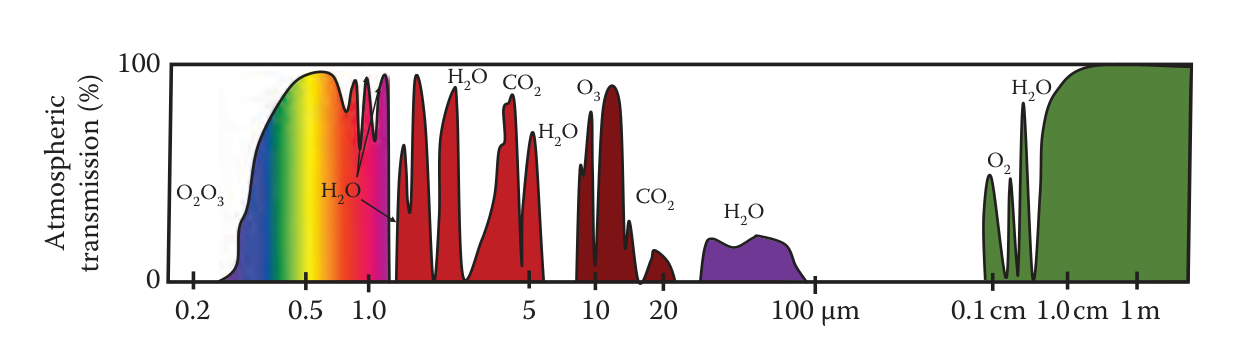
\includegraphics[width=1\textwidth]{Images/VentanasAtmosfericas.png}
    \end{center}
    \caption{Ventanas atmosféricas vistas a través del porcentaje de transmisión atmosférica.}
    \reference{Datos tomados de \citeA{chuvieco2016fundamentals}.}
    \label{fig:VentanasAtmosféricas}
\end{figure}

\textbf{b) Dispersión atmosférica}

Este fenómeno sucede cuando el entorno atmosférico, compuesto por diversos gases, aerosoles y vapor de agua, interactúa directamente con la radiación electromagnética, ocasionando que esta se desvíe de su trayectoria original \cite{canada2007fundamentals}.

La diversidad de los tamaños de las partículas presentes en la atmósfera da lugar a diferentes tipos de dispersión: Rayleigh, Mie y la dispersión no selectiva.

\textit{Dispersión de Rayleigh}: La dispersión de Rayleigh es especialmente sensible a la longitud de onda de la radiación incidente, lo cual afecta significativamente a las bandas de longitud de onda más corta. Esta dispersión se da cuando la radiación electromagnética interactúa con partículas que son más pequeñas que las longitudes de onda, como por ejemplo, las de moléculas de nitrógeno ($NO_{2}$) y oxígeno ($O_{2}$) \cite{tempfli2009principles, chuvieco2016fundamentals}. Un ejemplo claro de este tipo de dispersión es el cielo, ya que debido a la longitud de onda más corta dentro del espectro visible, se puede ver el cielo azul \cite{canada2007fundamentals}, tal y como se puede ver en la Figura~\ref{fig:DispersionRayleigh}.

\begin{figure}[H]
    \begin{center}
        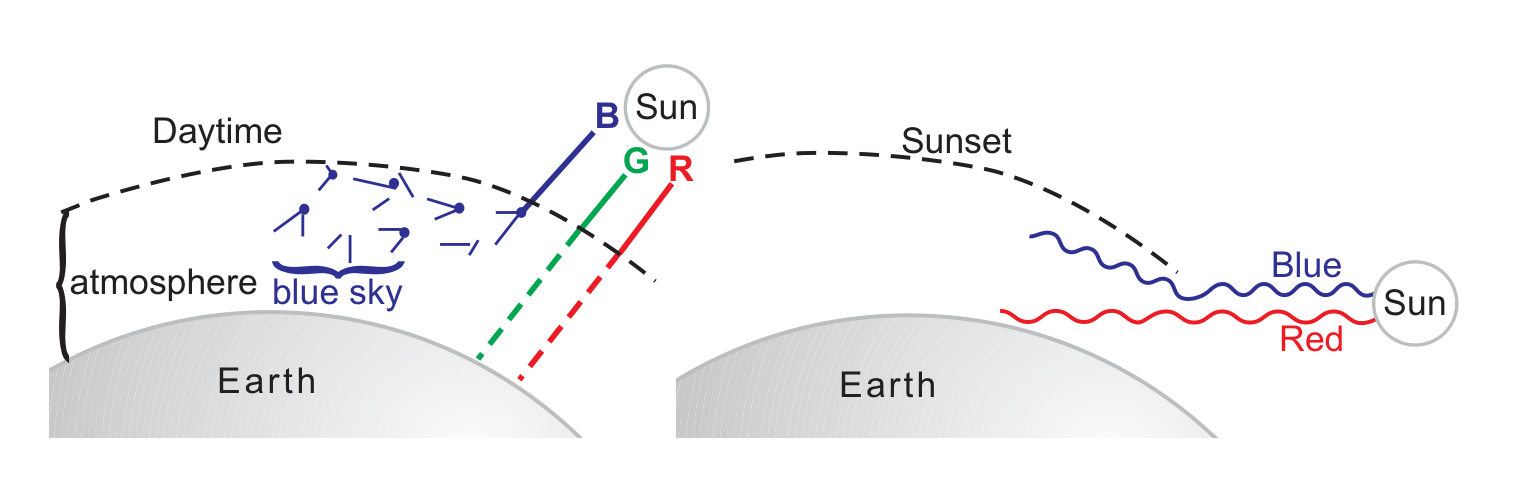
\includegraphics[width=1\textwidth]{Images/DispersionRayleigh.png}
    \end{center}
    \caption{Efectos de la dispersión de Rayleigh en el color del cielo.}
    \reference{Datos tomados de \citeA{tempfli2009principles}.}
    \label{fig:DispersionRayleigh}
\end{figure}

La dispersión de Rayleigh perturba la percepción remota en el rango espectral visible, particularmente desde altitudes elevadas. Esta interrupción provoca una distorsión en las características espectrales de la luz reflejada, resultando en una sobreestimación de las longitudes de onda más cortas y una tonalidad azulada en las imágenes capturadas, especialmente cuando se usan sensores multiespectrales \cite{tempfli2009principles}.

\textit{Dispersión de Mie}: Depende también de la longitud de onda incidente, pero su influencia es menor en comparación con la radiación de Rayleigh. Ocurre generalmente cuando las partículas tienen aproximadamente el mismo tamaño de la longitud de onda de la radiación \cite{canada2007fundamentals}. Esta dispersión se da generalmente en la atmósfera baja, donde hay una mayor abundancia de partículas grandes, y domina en condiciones de nubes cubiertas, teniendo un influencia en en el rango espectral desde el cercano ultravioleta hasta el infrarrojo medio \cite{tempfli2009principles}. En este tipo de dispersión, los elementos que son especialmente responsables son las partículas de aerosoles y el polvo atmosférico. Sin embargo, otros elementos como incendios forestales o niebla costera pueden ocasionarla \cite{chuvieco2016fundamentals}.

\textit{Dispersión no selectiva}: Esta se distingue por influir sobre todas las longitudes de onda por igual \cite{canada2007fundamentals, chuvieco2016fundamentals}. Es precisamente este fenómeno el que posibilita que nuestros ojos perciban las nubes y la niebla en tonos grises o blancos. Dado que las nubes están compuestas por gotas de agua, estas dispersan la luz de todas las longitudes de onda de manera uniforme, dando lugar a la apariencia blanca o grisácea que caracteriza a estos fenómenos atmosféricos \cite{tempfli2009principles}.

Dependiendo del tipo de tarea, en algunos casos es necesario realizar una corrección de la dispersión atmosférica. Este proceso permite obtener una estimación más precisa de la radiación superficial \cite{chuvieco2016fundamentals}.

\textbf{c) Emisión atmosférica}

Se refiere a la energía radiante emitida por la atmósfera, particularmente significativa en el espectro infrarrojo térmico (TIR). Este fenómeno es una consideración vital en la interpretación de imágenes satelitales, ya que puede influir en la precisión de la medida de la temperatura superficial. Cada cuerpo con una temperatura superior al cero absoluto, incluyendo la atmósfera, emite energía radiante, que puede ser detectada por sensores satelitales \cite{chuvieco2016fundamentals}.

\subsubsection{Interacción de la radiación electromagnética con la superficie terrestre}

La radiación que ni se absorbe ni se dispersa en la atmósfera finalmente entra en contacto con la superficie terrestre. Esta interacción puede manifestarse de tres formas: absorción, transmisión o reflexión. Las proporciones en las que cada una de estas ocurre dependen tanto de la longitud de onda de la energía incidente como de las propiedades y condiciones del material en la superficie terrestre \cite{canada2007fundamentals}.

En el campo de la teledetección, la radiación solar actúa como la principal fuente de radiación electromagnética. Aunque esta radiación interactúa significativamente con la atmósfera, una porción de esta energía logra llegar a la superficie terrestre. Al hacer contacto con la superficie, se manifiesta en las tres formas de interacción mencionadas anteriormente: absorción, transmisión y reflexión. Por lo tanto, se puede decir que la radiación entrante ($\phi_{i}$) se distribuirá entre ser reflejada ($\phi_{r}$), transmitida ($\phi_{t}$) o absorbida ($\phi_{a}$) \cite{chuvieco2016fundamentals}.

\begin{equation}
    \phi_{i} = \phi_{r} + \phi_{t} + \phi_{a}
\end{equation}

\begin{figure}[H]
    \begin{center}
        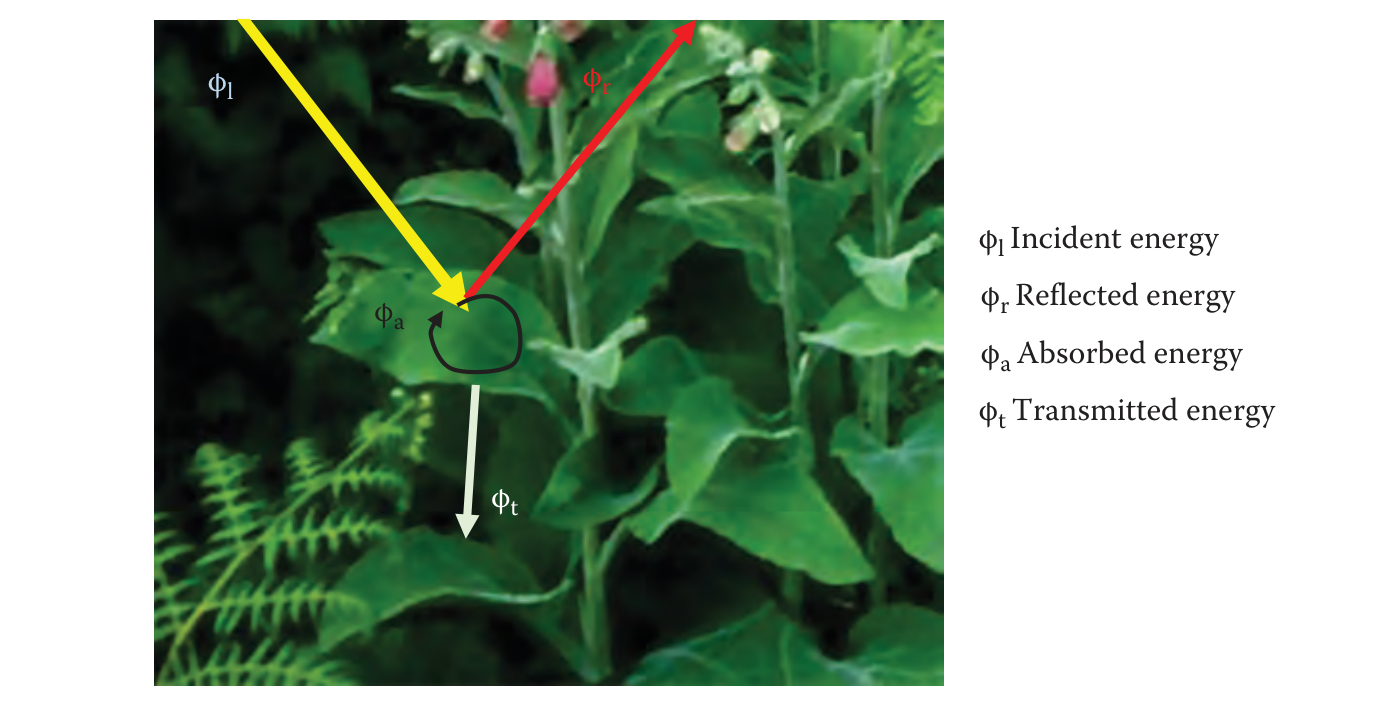
\includegraphics[width=0.95\textwidth]{Images/InteraccionSuperficie.png}
    \end{center}
    \caption{Interacción de la radiación electromagnética con la superficie terrestre.}
    \reference{Datos tomados de \citeA{chuvieco2016fundamentals}.}
    \label{fig:InteraccionSuperficie}
\end{figure}

La absorción ocurre cuando la radiación es asimilada por el objeto, la transmisión tiene lugar cuando la radiación atraviesa el objeto, y la reflexión sucede cuando la radiación rebota en el objetivo y es redirigida (ver Figura~\ref{fig:InteraccionSuperficie}). En el campo de la teledetección, se utiliza principalmente la radiación reflejada, ya que esta provee características significativas de la superficie terrestre al sensor remoto \cite{canada2007fundamentals, tempfli2009principles, chuvieco2016fundamentals}.

Existen dos tipos de reflexión: la reflexión especular y la reflexión difusa.

\textit{Reflexión especular}: Ocurre principalmente en superficies lisas, donde la radiación se refleja de manera casi uniforme en una sola dirección. Ejemplos comunes de esto incluyen la superficie del agua o el techo de un invernadero.

\textit{Reflexión difusa}: Tiene lugar cuando la superficie es rugosa, provocando que la radiación se refleje en múltiples direcciones de manera casi uniforme.

La manera en que un objeto refleja la radiación, ya sea de forma especular, difusa o una combinación de ambas, depende de la rugosidad de su superficie en relación con la longitud de onda de la radiación incidente \cite{tempfli2009principles}. La mayoría de las superficies exhiben características que se ubican en un punto intermedio entre estos dos extremos \cite{canada2007fundamentals}. Esta interacción singular da lugar a patrones de reflectancia que se identifican como ``firma espectral'', funcionando como una huella dactilar única para cada superficie y permitiendo su diferenciación e identificación \cite{chuvieco2016fundamentals}.

\subsubsection{Firma espectral}

La firma espectral, también denominada curva espectral, representa la cantidad de radiación incidente que se refleja en función de la longitud de onda, permitiendo así la identificación de objetos o materiales en una imagen de teledetección. Cada material posee una firma espectral única, determinada por sus propiedades físicas y químicas \cite{tempfli2009principles}. Por ejemplo, en el espectro visible y cercano al infrarrojo, la vegetación saludable suele reflejar gran cantidad de luz en las longitudes de onda verdes y del infrarrojo cercano, pero absorbe gran parte de la luz en las longitudes de onda rojas y azules. Esta interacción con la luz da a la vegetación su característico color verde \cite{emery2017introduction}.

Cada material posee una firma espectral única, determinada por sus características físicas y químicas \cite{chuvieco2016fundamentals}. Estas firmas permiten diferenciar diversos materiales presentes en una imagen de teledetección, facilitando así la elaboración de mapas que representan la distribución de estos materiales sobre la superficie terrestre (ver Figura \ref{fig:FirmasEspectralesSuperficie}).

\begin{figure}[H]
    \begin{center}
        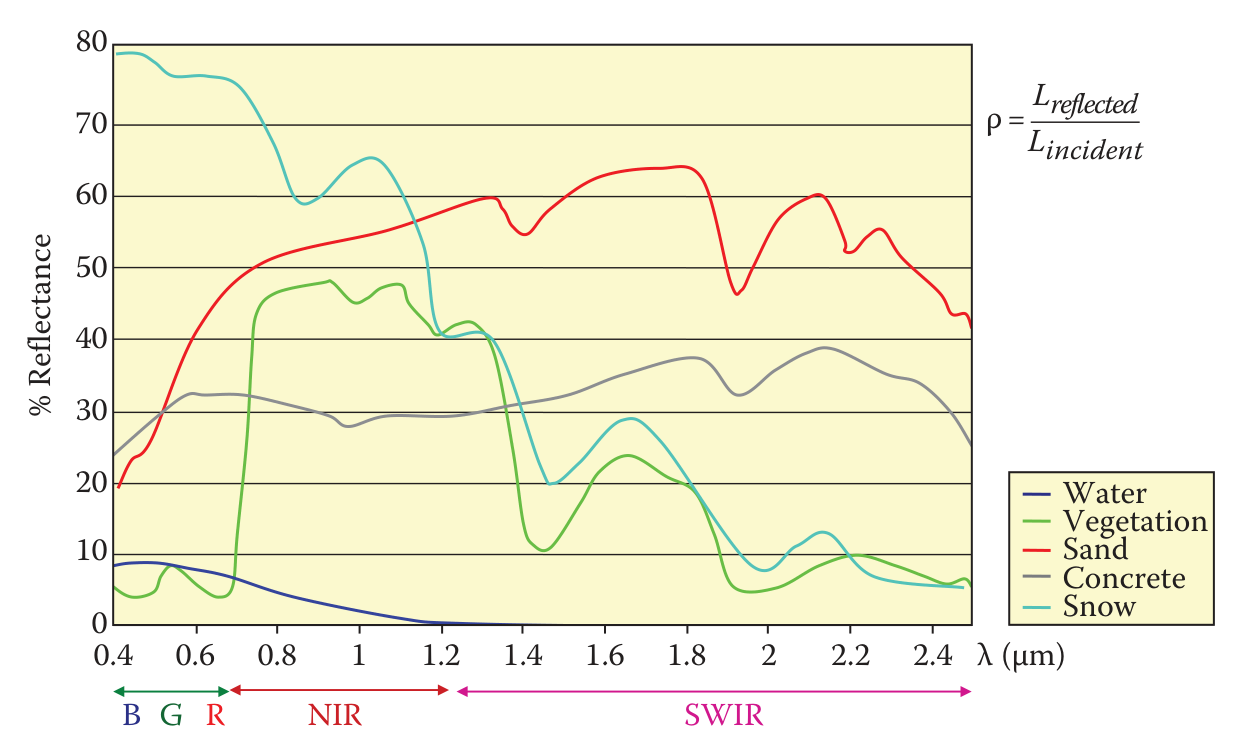
\includegraphics[width=1\textwidth]{Images/FirmasEspectralesSuperficie.png}
    \end{center}
    \caption{Firmas espectrales de los principales elementos de la superficie terrestre.}
    \reference{Datos tomados de \citeA{chuvieco2016fundamentals}.}
    \label{fig:FirmasEspectralesSuperficie}
\end{figure}

A pesar de que las firmas espectrales pueden facilitar la distinción entre diferentes materiales en la superficie terrestre, a menudo se encuentran diversos factores que pueden afectar su interpretación.

Tal como expone \citeA{chuvieco2016fundamentals}, existen múltiples elementos clave que pueden influir en las firmas espectrales (ver Figura~\ref{fig:FactorInfluenciaFirmasEspectrales}): (\textit{i}) Los componentes atmosféricos, que impactan en la absorción y dispersión de la radiación tanto entrante como reflejada. (\textit{ii}) Las variaciones en la cobertura del suelo que provocan cambios en la composición química o física, como por ejemplo la densidad, el contenido de pigmentos, la humedad o la rugosidad. Estas modificaciones pueden ser el resultado del ciclo estacional de la vegetación o los cultivos, las prácticas agrícolas, el pastoreo, entre otros. (\textit{iii}) El suelo y el sustrato geológico, especialmente importantes en áreas con cobertura vegetal limitada y dispersa, pues el sensor percibirá una señal más intensa procedente del suelo. (\textit{iv}) Las condiciones de iluminación solar, influenciadas por la latitud, el día del año y la hora del día. (\textit{v}) La pendiente del terreno. (\textit{vi}) El aspecto, que altera las condiciones de iluminación de una cobertura objetivo.

\begin{figure}[H]
    \begin{center}
        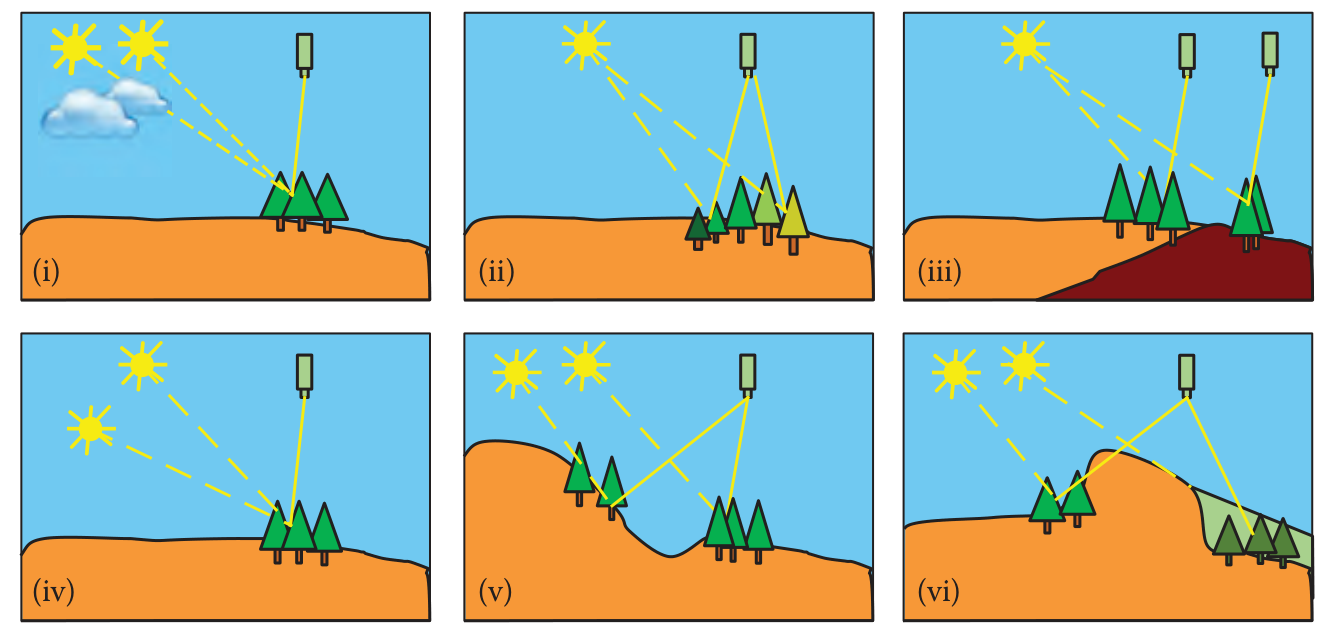
\includegraphics[width=1\textwidth]{Images/FactorInfluenciaFirmasEspectrales.png}
    \end{center}
    \caption{Factores que influencian en la composición de las firmas espectrales.}
    \reference{Datos tomados de \citeA{chuvieco2016fundamentals}.}
    \label{fig:FactorInfluenciaFirmasEspectrales}
\end{figure}

\subsubsection{Firmas espectrales}

\textbf{a) Vegetación}

La coloración verde característica de las plantas se debe en gran parte a la presencia de clorofila, un pigmento que absorbe entre un 60\% y 75\% de la energía en las longitudes de onda azul y roja \cite{chuvieco2016fundamentals}. La cantidad de clorofila varía a lo largo del año, siendo mayor o menor en las hojas según la estación. Además, las hojas sanas actúan como reflectores difusos en longitudes de onda cercanas al infrarrojo (NIR), aunque este comportamiento varía dependiendo del desarrollo de la hoja y su estructura celular. Este fenómeno permite medir y monitorear la salud de la vegetación \cite{canada2007fundamentals}. Adicionalmente, el contraste entre NIR y SWIR se utiliza a menudo para estimar el contenido de humedad de las hojas, ya que en el rango del SWIR, la reflectancia está mayormente determinada por la presencia de agua libre en el tejido de la hoja, de manera que una mayor cantidad de agua libre conlleva una menor reflectancia \cite{tempfli2009principles}.

\textbf{b) Agua}

Las longitudes de onda más largas del espectro visible y del infrarrojo cercano son absorbidas cuando interactúan con el agua, mientras que las longitudes de onda más cortas no, por lo que el agua se percibe de un tono azul o azul verdoso. El tinte verdoso es resultado de la presencia de algas en el agua, cuya clorofila absorbe más longitudes de onda azules y refleja las verdes \cite{canada2007fundamentals, tempfli2009principles}.

Comparada con la vegetación y los suelos, el agua tiene una reflectancia generalmente más baja. La vegetación puede reflejar hasta un 50\% de la energía incidente y los suelos hasta un 30-40\%, mientras que el agua apenas refleja un máximo del 10\%. La radiación reflejada por el agua se encuentra principalmente en el rango visible y, en menor grado, en el infrarrojo cercano, por lo que el resto de la energía es absorbida \cite{tempfli2009principles}.

Factores como la topografía y la presencia de sedimentos en la superficie del agua pueden dificultar la interpretación de las imágenes de teledetección debido a la reflexión especular, la cual afecta tanto el color como el brillo de la imagen \cite{canada2007fundamentals}. La rugosidad de la superficie del agua puede dar lugar a una reflexión difusa y dispersión, resultando en una mayor reflectancia. En aguas tranquilas, la reflexión es predominantemente especular, con una reflectancia altamente direccional y con valores variables dependiendo de los ángulos de visión y la dirección del sensor \cite{chuvieco2016fundamentals}.

\textbf{c) Hielo y nieve}

A diferencia del agua, la nieve exhibe una reflectancia muy elevada en las bandas visibles, disminuyendo considerablemente en el NIR y aún más en el SWIR. La reflectancia de la nieve está influenciada por factores como el tamaño de los cristales de nieve, la profundidad y densidad de la capa de nieve, así como la cantidad de impurezas que pueda contener. Cuando la nieve es más reciente, su reflectancia será mayor; por el contrario, será más baja a medida que envejece o se ensucia (ver Figura~\ref{fig:CurvasReflectanciaNieve}).

\begin{figure}[H]
    \begin{center}
        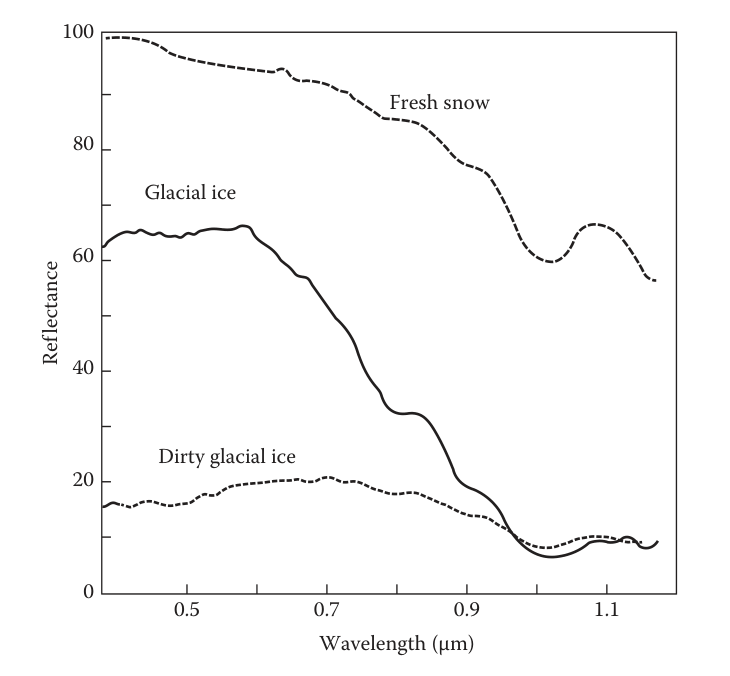
\includegraphics[width=0.8\textwidth]{Images/CurvasReflectancia.png}
    \end{center}
    \caption{Firma espectral de diferentes tipos de hielo y nieve.}
    \reference{Datos tomados de \citeA{chuvieco2016fundamentals}.}
    \label{fig:CurvasReflectanciaNieve}
\end{figure}

En el espectro visible, la nieve y las nubes suelen presentar retos para su diferenciación, debido a su similar alto índice de reflectancia. Sin embargo, este problema no persiste en el espectro SWIR. Los cristales de hielo o gotas de agua que constituyen las nubes son considerablemente más pequeños que los granos de nieve, resultando en una absorción menor de radiación en esta sección del espectro. A pesar de las dificultades en su identificación, la nieve por lo general exhibe una reflectancia ligeramente superior en las bandas visibles y una textura más uniforme en comparación a las nubes \cite{chuvieco2016fundamentals}.

\subsubsection{Características de la radiación electromagnética en la región del infrarrojo térmico del espectro electromagnético}

En la región del infrarrojo térmico (TIR) del espectro electromagnético, la radiación detectada por los sensores remotos proviene principalmente de la Tierra, ya que la reflexión de la radiación solar es mínima. Esto convierte la región del TIR en una herramienta útil para detectar cambios de temperatura en el suelo y la atmósfera.

La temperatura de un objeto está relacionada con su capacidad para absorber la radiación solar incidente. Si se considera que la suma de la reflectancia, transmisión y absorción es igual a 1, es decir, $1=\rho+\alpha+\tau$, y asumimos que la transmisión es $0$ en la región del TIR, la ecuación se simplifica a $1=\rho+\alpha$. Según la ley de Kirchhoff, la emisividad de un objeto es igual a su capacidad de absorción, lo que significa que cuanto mayor sea su absorción, mayor será su emisión. Por lo tanto, se llega a la siguiente ecuación:

\begin{equation}
    1=\rho+\epsilon
\end{equation}

donde:
\begin{itemize}
    \item $\rho$ es la reflectancia.
    \item $\epsilon$ es la emisividad del objeto.
\end{itemize}

Esto implica que los objetos con alta reflectancia absorberán poca radiación electromagnética y, como consecuencia, su nivel de emisividad será bajo. En la superficie terrestre, los elementos que emiten más son el agua y la vegetación densa, mientras que los suelos arenosos, la nieve y los metales muestran una emisividad menor.

Otros factores que influyen en el comportamiento térmico de un objeto son la capacidad térmica ($C$), la conductividad térmica ($k$), la difusividad térmica ($K$) y la inercia térmica ($P$) \cite{chuvieco2016fundamentals}.

En el Cuadro~\ref{tab:PropiedadesTIR} se detallan las propiedades de algunas de las coberturas de la superficie terrestre más comunes.

\begin{table}[H]
    \caption{Propiedades de las principales superficies terrestres en la región del infrarrojo térmico del espectro electromagnético.}
    \small
    \begin{tabularx}{1\textwidth}{lX}
        \hline
        \textbf{Superficie terrestre} & \textbf{Propiedades}                                                                                                                                                                                                                                                                                                                                                                                                                                                                                                                                                                        \\ \hline
        \textbf{Vegetación}           & La vegetación interactúa con una variedad de factores como la radiación solar, la fotosíntesis y la liberación de calor. Gracias a su alto contenido de agua, la vegetación presenta una considerable resistencia a los cambios bruscos de temperatura. Durante el día, la temperatura de las plantas tiende a disminuir debido a los procesos de transpiración. Por el contrario, durante la noche, la radiación absorbida durante el día se emite en forma de radiación térmica, lo que provoca un aumento en la temperatura de la vegetación, manteniendo así, su equilibrio energético. \\  \hline
        \textbf{Agua}                 & El agua presenta una notable resistencia a los cambios de temperatura debido a su alta conductividad térmica. La radiación incidente es absorbida de manera intensa y transmitida a lo largo de toda la superficie acuática. Este proceso contribuye a la notable estabilidad de la temperatura del agua.                                                                                                                                                                                                                                                                                   \\  \hline
        \textbf{Hielo y nieve}        & Las coberturas de nieve, debido a su menor emisividad de radiación electromagnética, registran temperaturas más bajas en comparación con su entorno. Esto se debe no solo a su alta reflectancia, sino también a otros factores como el tamaño de los cristales de nieve y su contenido de agua.                                                                                                                                                                                                                                                                                            \\  \hline
    \end{tabularx}
    \begin{minipage}{\textwidth}
        \vspace{10pt}
        \reference{Datos tomados de \cite{chuvieco2016fundamentals}.}
        \label{tab:PropiedadesTIR}
    \end{minipage}
\end{table}

\subsubsection{Características de la radiación electromagnética en la región de las microondas del espectro electromagnético}

Las microondas representan la región del espectro electromagnético que contiene longitudes de onda más largas. Esta región se diferencia de las mencionadas anteriormente, debido a que no depende de datos ópticos, es decir, datos derivados de la luz visible o cercana a esta \cite{tempfli2009principles}.

En la teledetección, las microondas se segmentan en diversas sub regiones según su longitud de onda. Cada una de estas sub regiones se representan mediante un carácter alfabético, como se muestra en el Cuadro~\ref{tab:BandasMW}.

\begin{table}[H]
    \caption{Representación de las sub regiones de las microondas utilizadas en la teledetección.}
    \small
    \begin{tabularx}{1\textwidth}{Xccc}
        \hline
        \textbf{Nombre \hspace{1cm}} & \textbf{\hspace{0.5cm}Longitud ($cm$)\hspace{0.5cm}} & \textbf{\hspace{0.5cm}Valor central ($cm$)\hspace{0.5cm}} & \textbf{Frecuencia ($GHz$)} \\ \hline
        $Ka$                         & 0.75 - 1.10                                          &                                                           &                             \\
        $K$                          & 1.10 - 1.67                                          & 1.0                                                       & 10.9 - 36                   \\
        $Ku$                         & 1.67 - 2.40                                          &                                                           &                             \\ \hline
        $X$                          & 2.40 - 3.75                                          & 3.0                                                       & 5.75 - 10.90                \\ \hline
        $C$                          & 3.75 - 7.50                                          & 5.6                                                       & 3.90 - 5.75                 \\ \hline
        $S$                          & 7.50 - 15.00                                         & 10.0                                                      & 1.55 - 3.90                 \\ \hline
        $L$                          & 15.00 - 30.00                                        & 23.0                                                      & 0.39 - 1.55                 \\ \hline
        $P$                          & 30.00 - 100.00                                       & 70.0                                                      & > 0.39                      \\ \hline
    \end{tabularx}
    \begin{minipage}{\textwidth}
        \vspace{10pt}
        \reference{Datos tomados de \cite{chuvieco2016fundamentals}.}
        \label{tab:BandasMW}
    \end{minipage}
\end{table}

Una de las principales características de esta región es su alta capacidad de transmisión atmosférica, lo que significa que es posible observar áreas sin importar las condiciones climáticas, superando así limitaciones comunes de otros métodos de teledetección, esto es debido a que las longitudes de onda son más grandes que el tamaño promedio de las partículas y moléculas presentes en la atmósfera (ver Figura~\ref{fig:LongitudOndaMW}).

\begin{figure}[H]
    \begin{center}
        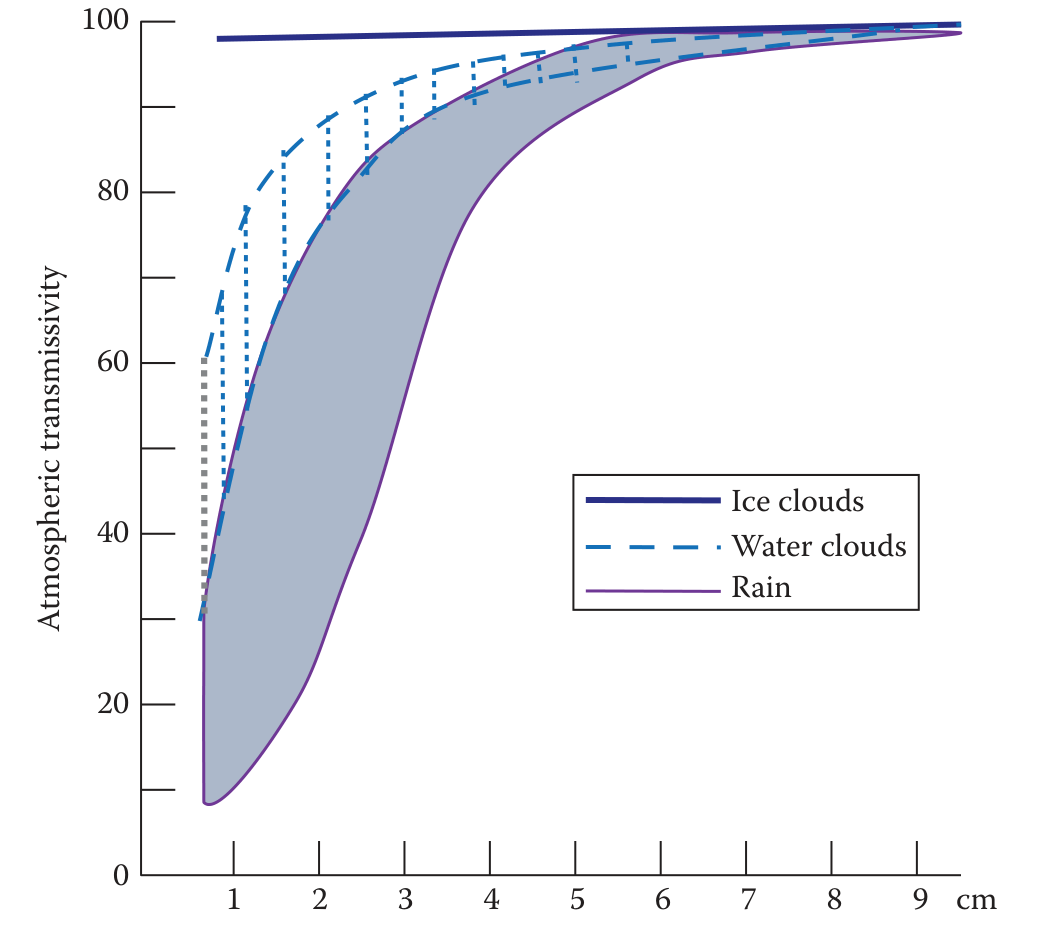
\includegraphics[width=0.8\textwidth]{Images/LongitudOndaMW.png}
    \end{center}
    \caption{Capacidad de transmisión atmosférica en la región de las microondas.}
    \reference{Datos tomados de \citeA{chuvieco2016fundamentals}.}
    \label{fig:LongitudOndaMW}
\end{figure}

Las observaciones remotas en esta región espectral se realizan mayormente con sensores activos, como el radar, que emiten y detectan energía de microondas desde la superficie. No obstante, también existen radiómetros pasivos de microondas, que recogen radiación de la superficie de forma similar a los sensores ópticos \cite{chuvieco2016fundamentals}.

En el Cuadro~\ref{tab:PropiedadesMW} se detallan las propiedades de algunas de las coberturas de la superficie terrestre más comunes.

\begin{table}[H]
    \caption{Propiedades de las principales superficies terrestres en la región de las microondas del espectro electromagnético.}
    \small
    \begin{tabularx}{1\textwidth}{lX}
        \hline
        \textbf{Superficie terrestre} & \textbf{Propiedades}                                                                                                                                                                                                                                                                                                                                                                                                                                                                                                                                                                                                                                                    \\ \hline
        \textbf{Vegetación}:          & La vegetación tiende a tener una respuesta espectral en la región de las microondas que es bastante compleja y depende de varios factores, incluyendo el tipo de vegetación, su etapa de crecimiento, y las condiciones ambientales. La vegetación, debido a su estructura tridimensional (hojas, ramas y tallos), interactúa con las microondas de una manera característica que se puede detectar. Las ondas de microondas pueden penetrar la vegetación y reflejar de manera más fuerte las estructuras más densas, como el tallo y las ramas de los árboles. Esta capacidad de penetración también permite la detección de la humedad del suelo bajo la vegetación.
        \\  \hline
        \textbf{Agua}:                & El agua, especialmente el agua de mar, tiene una firma espectral muy baja en la región de las microondas debido a su alta capacidad para absorber las ondas de radio. Por eso, los cuerpos de agua suelen aparecer muy oscuros en las imágenes de radar. La superficie del agua puede reflejar las microondas, pero la señal que llega al sensor es muy débil debido a la absorción.                                                                                                                                                                                                                                                                                    \\  \hline
        \textbf{Hielo y nieve}:       & Los sensores de microondas pasivos son muy útiles para monitorear el hielo marino, ya que son más sensibles a las temperaturas frías que los sensores ópticos. El hielo marino y el hielo de agua dulce también tienen firmas espectrales distintas debido a las diferencias en su estructura y composición.                                                                                                                                                                                                                                                                                                                                                            \\  \hline
    \end{tabularx}
    \begin{minipage}{\textwidth}
        \vspace{10pt}
        \reference{Datos tomados de \cite{chuvieco2016fundamentals}.}
        \label{tab:PropiedadesMW}
    \end{minipage}
\end{table}

\subsubsection{Plataformas}

Las plataformas son consideradas vehículos en movimiento, tales como satélites, aviones o vehículos aéreos no tripulados, empleados para diversas actividades específicas y conformados por diversos equipos o instrumentos \cite{tempfli2009principles}. Son de vital importancia ya que alojan los sensores encargados de obtener la información de la radiación electromagnética reflejada o incidente desde la Tierra \cite{chuvieco2016fundamentals}.

En función de su localización, las plataformas de teledetección se clasifican en terrestres, aéreas y espaciales \cite{canada2007fundamentals}. La utilidad de cada tipo de plataforma se determina según las necesidades específicas de la aplicación en cuestión. En el contexto de la teledetección, estas plataformas pueden operar desde alturas tan bajas como unos pocos centímetros, con el uso de equipamiento de campo, hasta posiciones en órbitas geoestacionarias a aproximadamente 36,000 km de distancia de la Tierra (ver Figura~\ref{fig:PlataformasTeledeteccion}) \cite{tempfli2009principles}.

\begin{figure}[H]
    \begin{center}
        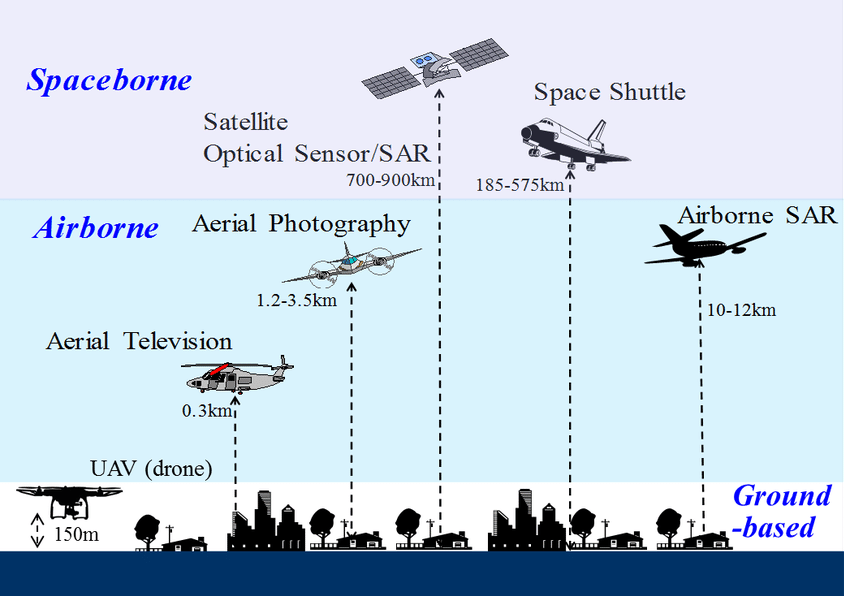
\includegraphics[width=1\textwidth]{Images/Plataformas.png}
    \end{center}
    \caption{Plataformas de teledetección.}
    \reference{Datos tomados de \citeA{yamazaki2016remote}.}
    \label{fig:PlataformasTeledeteccion}
\end{figure}

\textbf{a) Plataformas terrestres:} Conocidas también como \textit{Ground-based} en la jerga anglosajona, las plataformas terrestres ofrecen un alto nivel de detalle sobre zonas específicas, gracias a la cercanía entre el sensor y el área objeto de estudio. Comúnmente, se emplean estructuras elevadas como torres, edificios o grúas para su instalación \cite{canada2007fundamentals}. No obstante, esta categoría también abarca vehículos aéreos no tripulados, conocidos como Drones, que operan a una altitud máxima de aproximadamente 150 metros desde el nivel del suelo \cite{yamazaki2016remote}.

\textbf{b) Plataformas aéreas:} En inglés se denominan \textit{Airborne}. Aeronaves, sean aviones de ala fija o helicópteros, ofrecen la capacidad de cubrir vastas áreas geográficas en un tiempo relativamente corto. Operan a altitudes que van desde los 0.3 km hasta los 12 km sobre la superficie terrestre \cite{tempfli2009principles, yamazaki2016remote}. La flexibilidad en velocidad y altitud de estos vehículos influye directamente en la resolución y la escala de las imágenes obtenidas \cite{canada2007fundamentals}. Sin embargo, elementos como el viento y la orientación del vehículo pueden afectar la calidad del dato recogido \cite{tempfli2009principles}.

\textbf{c) Plataformas espaciales:} O \textit{Spaceborne} en inglés, proporcionan una perspectiva más global y tienen la ventaja de capturar datos de manera continua debido a sus órbitas específicas. Los satélites son los más comunes en esta categoría y suelen orbitar entre 700 y 900 km de altura respecto a la superficie terrestre. También existen vehículos espaciales que operan a altitudes que van desde los 185 hasta los 575 km desde la superficie terrestre \cite{tempfli2009principles}.

Los sensores terrestres son usualmente más asequibles pero tienen una cobertura limitada. Las plataformas aéreas ofrecen más flexibilidad pero incurren en mayores costos. Los satélites, aunque representan una inversión significativa, brindan la ventaja de un alcance global y una recopilación de datos constante \cite{canada2007fundamentals}.

\subsubsection{Sensores}

Los sensores en teledetección son dispositivos ubicados en plataformas de observación que miden y almacenan información a partir de la radiación electromagnética reflejada o emitida por la Tierra \cite{tempfli2009principles}.

\begin{figure}[H]
    \begin{center}
        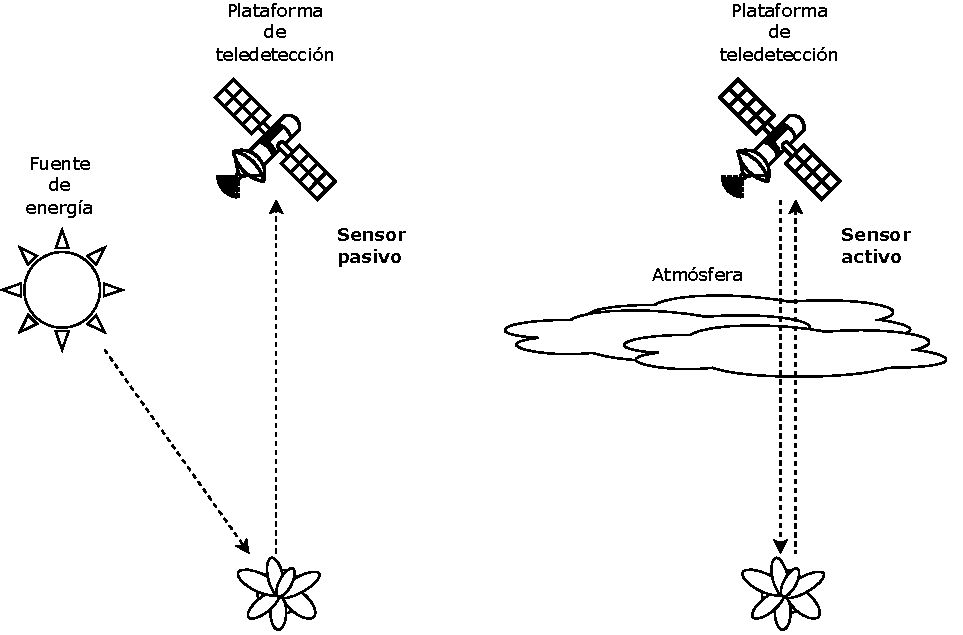
\includegraphics[width=1\textwidth]{Images/TipoSensores.pdf}
    \end{center}
    \caption{Tipos de sensores.}
    \reference{Elaborado por el autor.}
    \label{fig:TipoSensores}
\end{figure}

\textbf{a) Tipos de sensores}

Un enfoque habitual para clasificar los sensores en teledetección es según el método que emplean para captar información de la radiación electromagnética. Bajo este criterio, se distinguen principalmente dos tipos de sensores: activos y pasivos \cite{chuvieco2016fundamentals}.

\begin{itemize}
    \item \textit{Sensores pasivos:} Como se mencionó anteriormente, el Sol es la principal fuente de radiación electromagnética en la teledetección, lo que lo convierte en una fuente natural de energía. Estos sensores dependen de fuentes externas de energía como el Sol y, en algunos casos, la energía térmica de la Tierra (ver Figura~\ref{fig:TipoSensores}).

          Cubren un rango en el espectro electromagnético que va desde los rayos gamma hasta las microondas. Los ejemplos más comunes y antiguos de este tipo de sensores son las cámaras fotográficas y los escáneres electro ópticos \cite{tempfli2009principles, chuvieco2016fundamentals}. Sin embargo, tienen limitaciones; por ejemplo, su disponibilidad es limitada durante la noche, y su calidad depende de las condiciones climáticas de la atmósfera terrestre. Además, la radiación térmica emitida por la Tierra debe ser lo suficientemente intensa como para ser detectada por el sensor \cite{canada2007fundamentals}.

    \item \textit{Sensores activos:} La principal característica de este tipo de sensores es que son su propia fuente de energía (ver Figura~\ref{fig:TipoSensores}). Por lo tanto, las mediciones no dependen de factores externos como la luminosidad y el clima. Entre ellos se incluyen imágenes de Radar, LiDAR y Sonar. Un uso común de estos productos es para imágenes que representan altimetría \cite{tempfli2009principles, chuvieco2016fundamentals}.

          Estos sensores permiten obtener información de la radiación reflejada en cualquier momento del día y en cualquier estación del año. Además, tienen la capacidad de emitir radiación electromagnética en diversas longitudes de onda, a diferencia del Sol. Por ejemplo, las microondas pueden atravesar fácilmente la atmósfera terrestre gracias a su longitud de onda \cite{canada2007fundamentals}.
\end{itemize}

\subsubsection{Imágenes de teledetección}

La radiación electromagnética puede ser registrada tanto en fotografías como en imágenes. Tal como indica \citeA{canada2007fundamentals}, las imágenes y las fotografías presentan diferencias significativas. Las imágenes son representaciones digitales capturadas por cualquier tipo de dispositivo y pueden abarcar cualquier longitud de onda. Por otro lado, las fotografías se encuentran típicamente dentro del espectro visible y el infrarrojo, usualmente en un rango que va de $0.3 \mu m$ a $0.9 \mu m$.


\begin{figure}[H]
    \begin{center}
        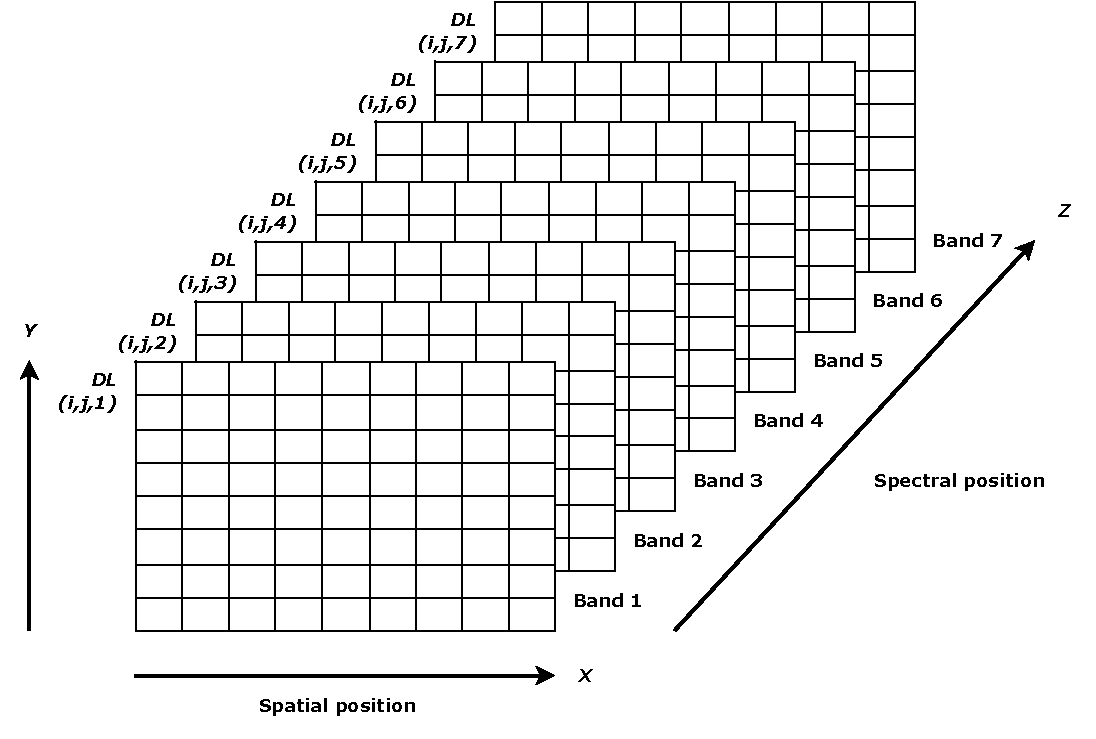
\includegraphics[width=1\textwidth]{Images/imagen_satelital.pdf}
    \end{center}
    \caption{Estructura y organización de los datos numéricos dentro de una imagen digital.}
    \reference{Datos tomados de \citeA{chuvieco2016fundamentals}.}
    \label{fig:ComposicionImagenSatelital}
\end{figure}

Las fotografías son consideradas imágenes, sin embargo, no todas las imágenes son necesariamente fotografías. En el ámbito digital, particularmente en teledetección, las imágenes se representan mediante matrices numéricas. Cada número de esta matriz corresponde a un píxel, la unidad más pequeña de una imagen. La Figura~\ref{fig:ComposicionImagenSatelital} ilustra cómo una imagen puede descomponerse en una matriz numérica en los ejes X e Y. Si la imagen tiene varias bandas, adquiere una estructura tridimensional en la que el eje Z representa diferentes bandas espectrales, lo cual es común en imágenes de teledetección ópticas \cite{chuvieco2016fundamentals}.

\textbf{a) Resolución de imágenes}

La teledetección se caracteriza por distintas modalidades de resolución que determinan su capacidad para captar y representar detalles en las imágenes. Uno de los aspectos más relevantes es la \emph{resolución espacial}.

\begin{itemize}
    \item \textit{Resolución espacial:} Se refiere al tamaño del píxel, expresado generalmente en metros, que indica la habilidad del sensor para discernir el objeto más pequeño en una imagen \cite{chuvieco2016fundamentals}. Esta resolución no sólo es una función del diseño del sensor, sino que está influenciada por la distancia entre el sensor y el objetivo. Específicamente, un sensor situado a una mayor altitud podrá abarcar un área geográfica más extensa en su toma, pero, con frecuencia, compromete la precisión en los detalles más finos. Por otro lado, aquellos sensores más cercanos al terreno, aunque limitados en la extensión del área que registran, son capaces de proporcionar un nivel de detalle notablemente superior \cite{canada2007fundamentals}.

          \begin{figure}[H]
              \begin{center}
                  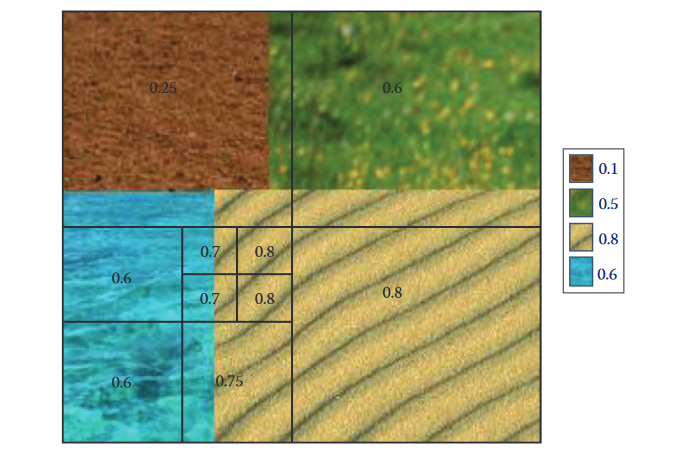
\includegraphics[width=1\textwidth]{Images/ResolucionEspacial.png}
              \end{center}
              \caption{Relación entre el tamaño del píxel y la capacidad de discriminación de los objetos en una imagen de teledetección.}
              \reference{Datos tomados de \citeA{chuvieco2016fundamentals}.}
              \label{fig:ResolucionEspacial}
          \end{figure}

          La elección adecuada de un sensor, en términos de su resolución espacial, es fundamental y debe estar alineada con los requerimientos específicos del estudio o aplicación en cuestión. Asimismo, es importante considerar que la resolución espacial incide directamente en la interpretación de las imágenes: mientras que imágenes de baja resolución son útiles para identificar características de mayor tamaño, aquellas con alta resolución permiten una detección e identificación más precisa de objetos más pequeños (ver Figura~\ref{fig:ResolucionEspacial}) \cite{canada2007fundamentals}.

    \item \textit{Resolución espectral:} Se refiere a la capacidad de un sensor para discernir la cantidad y el ancho de banda de los canales espectrales. Los sensores que cuentan con una elevada resolución espectral son capaces de identificar numerosas bandas delgadas a lo largo del espectro electromagnético. Sin embargo, aquellos sensores con resolución espectral más limitada perciben un número menor de bandas, que resultan ser más anchas \cite{chuvieco2016fundamentals}.

          \begin{figure}[H]
              \begin{center}
                  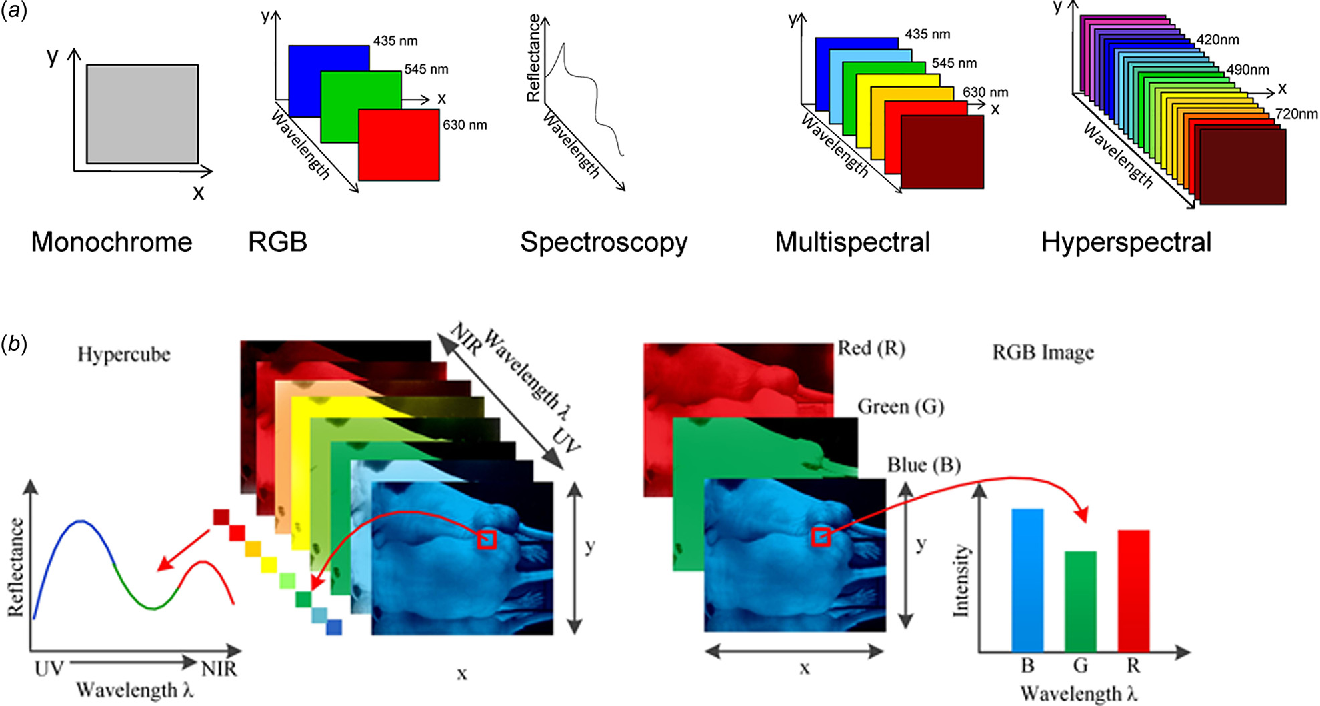
\includegraphics[width=1\textwidth]{Images/ResolucionEspectral.png}
              \end{center}
              \caption{Tipos de resolución espectral en una imagen de teledetección.}
              \reference{Datos tomados de \citeA{mehta2018single}.}
              \label{fig:ResolucionEspectral}
          \end{figure}

          En la actualidad se pueden encontrar imágenes con una sola banda espectral, imágenes con las bandas del espectro visible, y según aumente su cantidad de canales, imágenes multiespectrales e imágenes hiperespectrales (ver Figura~\ref{fig:ResolucionEspectral}).

    \item \textit{Resolución radiométrica:} La resolución radiométrica indica la capacidad de un sensor para distinguir minúsculas variaciones en la radiancia espectral. En sistemas fotográficos, determina la cantidad de niveles de grises que pueden ser almacenados. En sensores ópticos electrónicos, esta resolución establece el rango de valores usados para registrar la radiación electromagnética entrante \cite{chuvieco2016fundamentals}. Computacionalmente, un valor se representa como un «0» o un «1». Si se dice que una imagen es de 8 bits, esto supone un total de \(2^8\) o 256 posibles combinaciones (lo que indica el rango de valores que puede tomar el píxel) \cite{tempfli2009principles}.

          \begin{figure}[H]
              \begin{center}
                  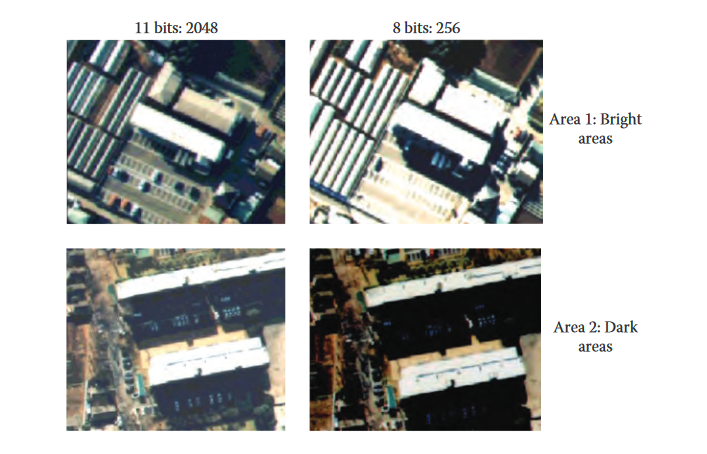
\includegraphics[width=1\textwidth]{Images/ResolucionRadiometrica.png}
              \end{center}
              \caption{Comparación visual de imágenes con diferentes resoluciones radiométricas (11 bits y 8 bits).}
              \reference{Datos tomados de \citeA{chuvieco2016fundamentals}.}
              \label{fig:ResolucionRadiometrica}
          \end{figure}

          Como señala \citeA{chuvieco2016fundamentals}, la resolución radiométrica es crucial en el análisis digital en comparación con el análisis visual. Esto se debe a que el ojo humano solo puede discernir alrededor de 64 niveles de gris y no más de 200.000 colores. Sin embargo, en sistemas de análisis digitales, esta resolución es fundamental para diferenciar objetos con firmas espectrales semejantes, tarea que sería inviable con sensores de menor sensibilidad tal y como se muestra en la Figura~\ref{fig:ResolucionRadiometrica}.

    \item \textit{Resolución temporal:} Hace referencia a la periodicidad con la que un satélite pasa por un punto específico de la superficie terrestre, es decir, el intervalo de tiempo entre dos observaciones consecutivas del mismo lugar \cite{tempfli2009principles, chuvieco2016fundamentals}. Esta resolución es importante para monitorear fenómenos en constante cambio, como el desarrollo de cultivos o la expansión urbana. Por ejemplo, el seguimiento de fenómenos climáticos rápidos requiere resoluciones temporales cortas, mientras que el estudio de cambios geológicos puede basarse en observaciones más espaciadas \cite{canada2007fundamentals}.
\end{itemize}

\textbf{b) Tipos de imágenes}

Las imágenes obtenidas a través de la teledetección se diferencian principalmente por los sensores que se utilizan en su captura. Los principales tipos se detallan en el Cuadro~\ref{tab:TiposImagenesTeledeteccion}.

\begin{table}[H]
    \caption{Tipos de imágenes de teledetección.}
    \begin{tabularx}{1\textwidth}{p{4.5cm}X}
        \hline
        \textbf{Tipo de imagen}                       & \textbf{Descripción}                                                                                                                                                                                                                                                                              \\
        \hline
        Imagen multiespectral                         & Imágenes de múltiples bandas donde cada píxel representa la información de la radiancia o reflectancia de los objetos en la superficie terrestre.                                                                                                                                                 \\
        \hline
        Imagen pancromática                           & Imágenes de una banda que integran la información de las bandas del espectro visible e infrarrojo cercano, comúnmente con una mayor resolución espacial que las imágenes multiespectrales.                                                                                                        \\
        \hline
        Imagen fusionada \newline (Pan-Sharpened)     & Resultado de la fusión entre una imagen pancromática y una multiespectral. Se mantiene la resolución espacial de la imagen pancromática, pero se incorporan los valores del sensor multiespectral en cada banda. Esta combinación se logra mediante un proceso denominado ``Pansharpening''.      \\
        \hline
        Imagen de radar                               & Las imágenes de radar de apertura sintética (SAR) provienen de sensores activos y se generan a partir de datos en el rango de las microondas. Estas ondas pueden penetrar la atmósfera y proporcionar información independientemente de condiciones climáticas, nubosidad o visibilidad nocturna. \\
        \hline
        Imágenes termográficas                        & Provienen de sensores térmicos que proporcionan información sobre la temperatura de la superficie terrestre.                                                                                                                                                                                      \\
        \hline
        Modelos digitales de elevación \newline (DEM) & Son representaciones digitales de la altitud superficial de una zona determinada. Se obtienen mediante el procesamiento de fotografías aéreas, imágenes SAR, imágenes LiDAR o datos topográficos. Entre los modelos digitales de elevación más empleados se encuentran: SRTM y ASTER GDEM.        \\
        \hline
    \end{tabularx}
    \begin{minipage}{\textwidth}
        \vspace{10pt}
        \reference{Datos tomados de \citeA{bravo2017teledeteccion}.}
        \label{tab:TiposImagenesTeledeteccion}
    \end{minipage}
\end{table}
\subsection{Imágenes satelitales}

Las imágenes satelitales son representaciones gráficas adquiridas mediante sensores ubicados en satélites que orbitan alrededor de la Tierra. Estos satélites, además de proveer imágenes, tienen una diversidad de aplicaciones, como la comunicación, la navegación, la investigación científica y la observación terrestre \cite{canada2007fundamentals}.

Dentro de los satélites empleados en teledetección, los más destacados son los satélites de observación \cite{canada2007fundamentals}. Estos están equipados con sensores que capturan información mediante la radiación electromagnética reflejada o emitida por la superficie terrestre y otros fenómenos atmosféricos. Además de los satélites de observación, existen otros que se dedican al monitoreo climático, posicionamiento (como los GPS), y estudios atmosféricos, por mencionar algunos \cite{jensen2016introductory}.

Cada imagen satelital se almacena en estructuras de datos multi dimensionales, comúnmente matrices, en donde cada elemento representa la información detectada por el sensor \cite{chuvieco2016fundamentals}. Dependiendo de la etapa de procesamiento en la que se encuentre la imagen, estos elementos pueden representar valores digitales, valores de radiancia o valores de reflectancia.

\subsubsection{Niveles de procesamiento}

Los niveles de procesamiento indican los tratamientos aplicados a la información originalmente capturada por el sensor. Estos procesamientos influencian en los valores registrados en la imagen satelital, que pueden categorizarse según su nivel de procesamiento, como se detalla en el Cuadro~\ref{tab:NivelProcesamientoImagenSatelital}.

\begin{table}[H]
    \caption{Niveles de procesamiento de una imagen satelital.}
    \begin{tabularx}{1\textwidth}{p{4cm}X}
        \hline
        \textbf{Nivel de  \newline procesamiento} & \textbf{Descripción}                                                                                                                                                                                                                                                                                                                                                                          \\
        \hline
        Valores Digitales                         & Representan los datos inalterados que provienen directamente del sensor, ya sea en un satélite o en una aeronave. Corresponden a la cantidad de energía electromagnética percibida por el sensor y convertida en un número digital, comúnmente en una escala de 0 a 255 para imágenes de 8 bits. No han sido sujetos a correcciones o calibraciones.                                          \\
        \hline
        Valores de radiancia                      & Denotan una medida física de la energía electromagnética que emana de una fuente y es detectada por el sensor satelital. Esta se expresa en términos de potencia por unidad de área y por unidad de ángulo sólido. Los valores digitales se pueden transformar a valores de radiancia usando coeficientes de calibración suministrados por las agencias encargadas de los satélites.          \\
        \hline
        Valores de reflectancia                   & Indican la proporción de energía solar que, tras incidir en la superficie terrestre, es reflejada de vuelta al sensor. Se representa típicamente como un valor entre 0 y 1 o en porcentaje. Para transformar los valores de radiancia a reflectancia es necesario considerar aspectos como la distancia Tierra-Sol al momento de la captura, el ángulo solar y las correcciones atmosféricas. \\
        \hline
    \end{tabularx}
    \begin{minipage}{\textwidth}
        \vspace{10pt}
        \reference{Datos tomados de \citeA{jensen2016introductory}.}
        \label{tab:NivelProcesamientoImagenSatelital}
    \end{minipage}
\end{table}

\subsubsection{Niveles de corrección}

Cada nivel de corrección aborda distintas imperfecciones o distorsiones que pueden haberse introducido en diferentes etapas del proceso de adquisición.

\textbf{a) Corrección radiométrica}

Se restauran aquellos píxeles que puedan haberse visto afectados durante el proceso de adquisición de datos. Algunos píxeles pueden haberse deteriorado o incluso perdido. Para contrarrestar esto, se recurre a técnicas que estiman valores a partir de promedios adyacentes u otros métodos similares. Una distorsión común es el bandeado, originado por discrepancias en la calibración entre detectores. La corrección del bandeado se basa en la hipótesis de que, en ausencia de errores, los histogramas de cada detector deberían ser consistentes entre sí y, simultáneamente, alinearse con el histograma global de la imagen \cite{jensen2016introductory}.

\textbf{b) Corrección geométrica}

Las imágenes son sometidas a un proceso de georreferenciación, asignando a cada píxel una coordenada geográfica específica \cite{chuvieco2016fundamentals}. No obstante, al realizar esta operación, pueden introducirse distorsiones. Para rectificar estas imprecisiones, se adoptan medidas como la corrección orbital, la identificación de puntos de control en tierra, el cálculo de errores por mínimos cuadrados, y la integración de modelos digitales de elevación \cite{jensen2016introductory}.

\textbf{b) Corrección atmosférica}

La corrección atmosférica busca identificar y rectificar las distorsiones provocados por la presencia gases y partículas, garantizando que la información registrada por el sensor refleje de manera más precisa las condiciones reales en la superficie terrestre \cite{bravo2017teledeteccion}. Estas correcciones se fundamentan en modelos atmosféricos y algoritmos que consideran la composición y condiciones de la atmósfera en el momento de la captura \cite{jensen2016introductory}.

\subsubsection{Índices espectrales}

\textbf{a) NDVI}

El NDVI (Índice de Vegetación de la Diferencia Normalizada) es utilizado para estimar la cantidad, calidad y desarrollo de la vegetación. Basándose en cómo la vegetación refleja la luz en distintas partes del espectro, especialmente en las bandas roja y NIR, el NDVI es una métrica de la actividad fotosintética y salud de la vegetación. Un NDVI positivo generalmente indica áreas vegetadas, mientras que valores negativos o cercanos a cero pueden representar áreas no vegetadas o vegetación estresada \cite{rouse1974monitoring}.

\begin{equation*}
    NDVI = \frac{NIR - Red}{NIR + Red}
\end{equation*}

\textbf{b) NDWI}

El NDWI (Índice de Agua de la Diferencia Normalizada) se utiliza ampliamente para monitorear el contenido de agua en la vegetación y para identificar masas de agua. La versión que utiliza las bandas Green y NIR es efectiva para detectar el contenido de agua en la vegetación. Otras variantes del NDWI que emplean la banda SWIR son más adecuadas para identificar cuerpos de agua, ya que esta banda es más sensible a cambios en el contenido de agua en el suelo \cite{gao1996ndwi}.

\begin{equation*}
    NDWI = \frac{Green - NIR}{Green + NIR}
\end{equation*}

\textbf{C) NDSI}

El NDSI (Índice de Nieve de la Diferencia Normalizada) se utiliza para identificar y monitorizar la cobertura de nieve en áreas terrestres. Este índice es útil en áreas polares o montañosas y es esencial para estudios climáticos, hidrológicos y de gestión del agua, ya que la nieve tiene un papel crítico en el balance hídrico de muchas regiones \cite{dozier1989spectral}.

\begin{equation*}
    NDSI = \frac{Green - SWIR}{Green + SWIR}
\end{equation*}

\subsubsection{Sentinel-2}

Las imágenes satelitales de Sentinel-2 son generadas a partir de los sensores ubicados en las plataformas Sentinel-2A, y Sentinel-2B. Ambos satélites forman parte del programa espacial Copernicus de la Agencia Espacial Europea (ESA), y fueron lanzados el 23 de junio de 2015 y el del Sentinel-2B respectivamente. El objetivo principal de Sentinel-2, es el seguimiento de la vegetación, la cobertura del suelo, y los recursos hídricos, además de la observación de cuerpos de agua interiores y zonas costeras \cite{sentinel2}.

\begin{figure}[H]
    \begin{center}
        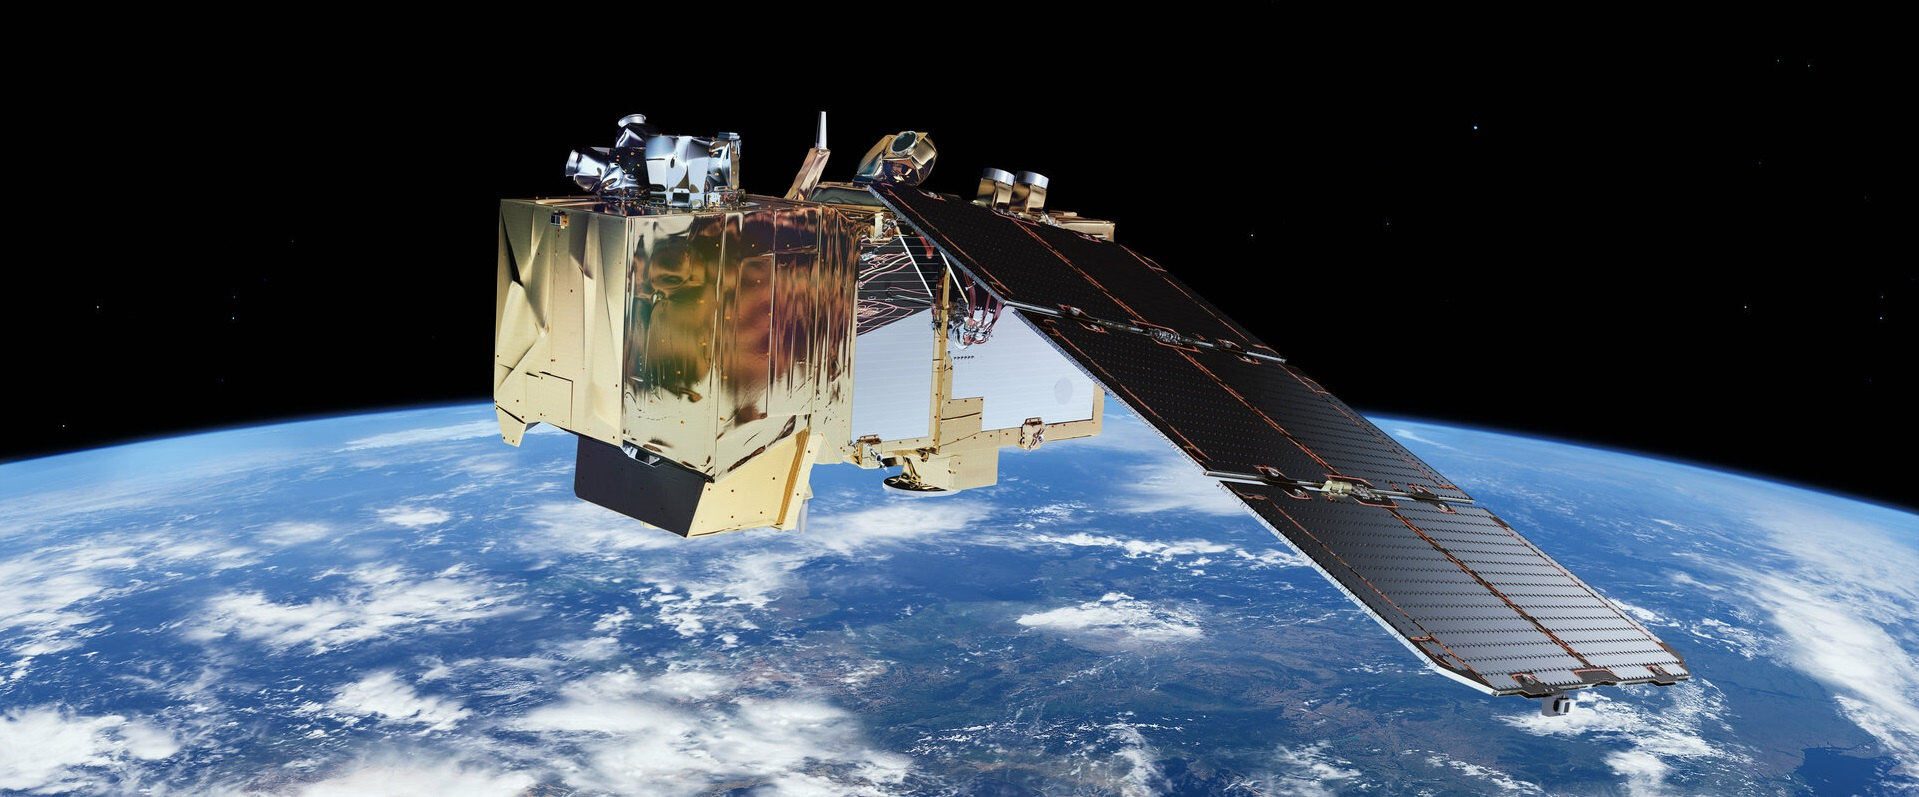
\includegraphics[width=1\textwidth]{Images/Sentinel2.jpg}
    \end{center}
    \caption{Plataforma Sentinel-2.}
    \reference{Datos tomados de \citeA{sentinel2}.}
    \label{fig:Sentinel2}
\end{figure}

Además de Sentinel-2, otras misiones espaciales relacionadas son Sentinel-1 y Sentinel-3. Sentinel-1 se compone de dos satélites, Sentinel-1A y Sentinel-1B (inoperativo), que cuentan con sensores activos, permitiendo la captura de datos independientemente del momento del día. Sentinel-1A fue puesto en órbita el 3 de abril de 2014. Con una frecuencia de adquisición de imágenes cada 6 días, estos satélites operan en la banda C y están orientados a ofrecer servicios terrestres y marinos. Algunas de sus aplicaciones incluyen el monitoreo de inundaciones, seguimiento de la superficie terrestre y análisis de patrones marinos.

Por otro lado, Sentinel-3, con sus satélites gemelos Sentinel-3A y Sentinel-3B, está equipado con una variedad de instrumentos: el Instrumento de Color Oceánico y Terrestre (OLCI), el Radiómetro de Temperatura de Superficie Terrestre y Marina (SLSTR), el Altímetro Radar SAR (SRAL) y el Radiómetro de Microondas (MWR). Estos instrumentos se enfocan tanto en el monitoreo marino como terrestre.

\textbf{a) Resoluciones}

Sentinel 2A y Sentinel 2B poseen características técnicas idénticas. Por este motivo, el Cuadro~\ref{tab:ResolucionesSentinel2} hace referencia a las resoluciones de ambos como Sentinel-2.

\begin{table}[H]
    \caption{Resoluciones de las imágenes Sentinel-2.}
    \small
    \begin{tabularx}{1\textwidth}{XX}
        \hline
        \textbf{Resolución}     & \textbf{Descripción}                                                                                                                                                                                                                                                                                    \\ \hline
        Resolución espacial     & La resolución espacial máxima de las imágenes Sentinel-2 es de 10 metros. No obstante, cada banda puede presentar una resolución espacial diferente, que puede ser de 10, 20 o 60 metros. Los detalles sobre la resolución espacial se encuentran especificados en el Cuadro~\ref{tab:BandasSentinel2}. \\ \hline
        Resolución espectral    & El sensor captura información en 13 bandas que abarcan desde el espectro visible e infrarrojo (VNIR) hasta el infrarrojo de onda corta (SWIR).                                                                                                                                                          \\ \hline
        Resolución radiométrica & Los productos obtenidos por el sensor, en términos de radiancia, poseen una resolución radiométrica de 12 bits (valores de píxeles de 0 a 4095). En contraste, los productos que representan la reflectancia se almacenan con números enteros de 16 bits.                                               \\ \hline
        Resolución temporal     & La resolución temporal de cada satélite es de 10 días, y la constelación combinada ofrece una resolución temporal de 5 días.                                                                                                                                                                            \\
    \end{tabularx}
    \begin{minipage}{\textwidth}
        \vspace{10pt}
        \reference{Datos tomados de \citeA{sentinel2}.}
        \label{tab:ResolucionesSentinel2}
    \end{minipage}
\end{table}

\textbf{b) Bandas}

Sentinel-2A y Sentinel-2B disponen de 13 bandas espectrales, es decir, se consideran como imágenes multiespectrales. Los detalles de cada banda se especifican en el Cuadro~\ref{tab:BandasSentinel2}.

\begin{table}[H]
    \caption{Información espectral de una imagen Sentinel-2.}
    \small
    \begin{tabularx}{1\textwidth}{p{6cm}XX}
        \hline
        \textbf{Banda}               & \textbf{Longitud de onda central (\textmu m)} & \textbf{Resolución espacial (m)} \\
        \hline
        Band 01: Coastal aerosol     & 0.443                                         & 60                               \\
        Band 02: Blue                & 0.490                                         & 10                               \\
        Band 03: Green               & 0.560                                         & 10                               \\
        Band 04: Red                 & 0.665                                         & 10                               \\
        Band 05: Vegetation Red Edge & 0.705                                         & 20                               \\
        Band 06: Vegetation Red Edge & 0.740                                         & 20                               \\
        Band 07: Vegetation Red Edge & 0.783                                         & 20                               \\
        Band 08: NIR                 & 0.842                                         & 10                               \\
        Band 8A: Vegetation Red Edge & 0.865                                         & 20                               \\
        Band 09: Water vapour        & 0.945                                         & 60                               \\
        Band 10: SWIR - Cirrus       & 1.375                                         & 60                               \\
        Band 11: SWIR                & 1.610                                         & 20                               \\
        Band 12: SWIR                & 2.190                                         & 20                               \\
        \hline
    \end{tabularx}
    \begin{minipage}{\textwidth}
        \vspace{10pt}
        \reference{Datos tomados de \citeA{sentinel2}.}
        \label{tab:BandasSentinel2}
    \end{minipage}
\end{table}

\textbf{c) Productos}

Los tipos de producto generados por Sentinel-2 se especifican en el Cuadro~\ref{tab:SentinelTipoProducto}.

\begin{table}[H]
    \caption{Tipos de productos disponibles en Sentinel-2.}
    \small
    \begin{tabularx}{1\textwidth}{XXXX}
        \hline
        \textbf{Nombre} & \textbf{Descripción de alto nivel}                                             & \textbf{Producción y distribución}            & \textbf{Tamaño}                \\ \hline
        Level-1B        & Radiancia, (TOA), en la geometría del sensor.                                  & Generación sistemática y distribución online. & 27 MB (cada 23x25 $km^{2}$)    \\
        Level-1C        & Reflectancia, (TOA), en la geometría cartográfica.                             & Generación sistemática y distribución online. & 500 MB (cada 110x110 $km^{2}$) \\
        Level-2A        & Reflectancia, (BOA), corregidas atmosféricamente en la geometría cartográfica. & Generación sistemática y distribución online. & 600 MB (cada 110x110 $km^{2}$) \\ \hline
    \end{tabularx}
    \begin{minipage}{\textwidth}
        \vspace{10pt}
        \reference{Datos tomados de \citeA{sentinel2}.}
        \label{tab:SentinelTipoProducto}
    \end{minipage}
\end{table}

Las imágenes L1C se encuentran ortorectificadas y con niveles de reflectancia superior a la atmósfera (TOA), mientras que las imágenes L2A se encuentran ortorectificadas y con noveles de reflectancia por debajo de la atmósfera (BOA). Es decir, las imágenes L2A presentan corrección atmosférica (ver Figura~\ref{fig:ComparacionBOATOA}).

\begin{figure}[H]
    \begin{center}
        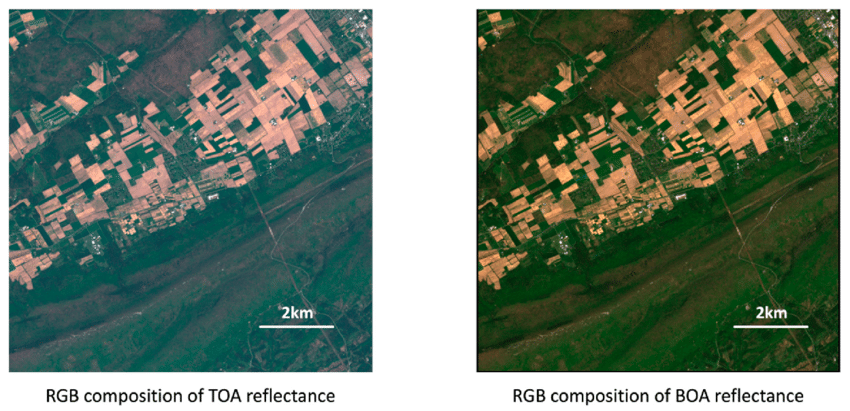
\includegraphics[width=1\textwidth]{Images/ComparacionBOATOA.png}
    \end{center}
    \caption{Comparación visual de dos imágenes (RGB) de Sentinel-2A: TOA, BOA.}
    \reference{Datos tomados de \citeA{song2020validation}.}
    \label{fig:ComparacionBOATOA}
\end{figure}

En el caso de las imágenes de nivel L1B, los productos se representan como ``gránulos'', los cuales abarcan un total de $23x25 km^2$ por cada uno. En el caso de las imágenes de nivel L1C y L2A, los productos representan ``mosaicos'', los cuales tienen un tamaño de $110x110 km^2$, los $10^2$ adicionales tienen el objetivo de evitar el solapamiento entre los mosaicos \cite{sentinel2}.

\subsubsection{Landsat}

Landsat es un programa de satélites de observación de la Tierra, el cual ha estado funcionando desde 1972 cuando se lanzó el primer satélite Landsat. Este programa es una colaboración entre la NASA y el USGS (Servicio Geológico de Estados Unidos)  \citeA{landsat}. La misión de Landsat es recopilar información sobre la superficie terrestre utilizando imágenes multiespectrales, proporcionando datos valiosos para la agricultura, cartografía, geología, silvicultura, planificación del uso del suelo y la educación, entre otras aplicaciones \cite{williams2006landsat}.


\begin{figure}[H]
    \begin{center}
        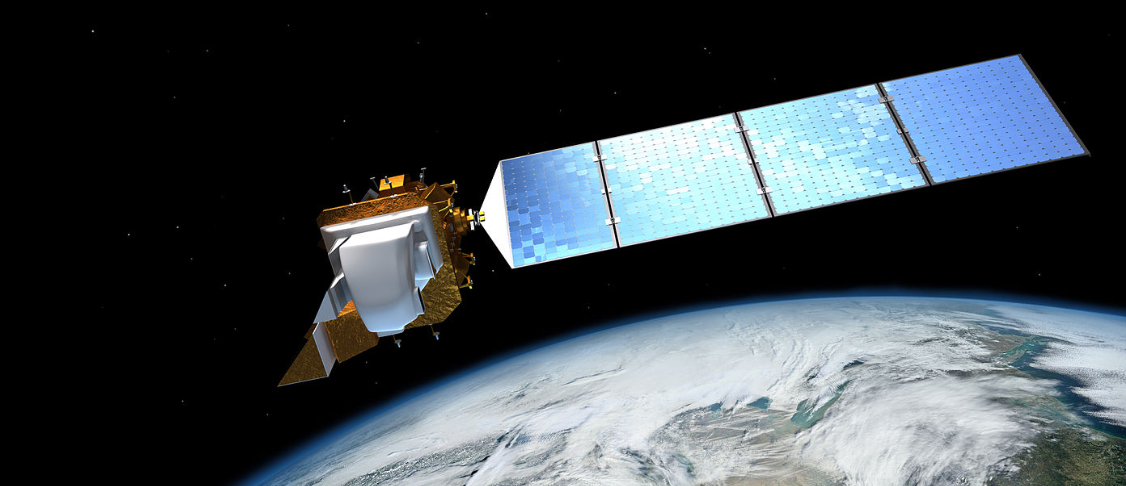
\includegraphics[width=1\textwidth]{Images/Landsat8.png}
    \end{center}
    \caption{Plataforma Landsat 8.}
    \reference{Datos tomados de \citeA{landsat}.}
    \label{fig:Landsat8}
\end{figure}

Los satélites Landsat recogen datos con resoluciones espaciales que pueden ser adecuadas para estudiar fenómenos a escala regional o global, y han sido fundamentales en el desarrollo de estudios sobre el cambio climático y la gestión de recursos naturales \cite{young2017land}. A lo largo de los años se han lanzado múltiples misiones Landsat. En el Cuadro~\ref{tab:ProgramaLandsat}, se detalla los años de lanzamiento y finalización de operaciones de cada satélite.

\begin{table}[H]
    \caption{Satélites del programa Landsat: Años de lanzamiento y finalización de operaciones.}
    \small
    \begin{tabularx}{1\textwidth}{p{2.5cm}p{5cm}X}
        \hline
        \textbf{Satélite Landsat} & \textbf{Año de lanzamiento} & \textbf{Año de finalización de operaciones} \\
        \hline
        Landsat 1                 & 1972                        & 1978                                        \\ \hline
        Landsat 2                 & 1975                        & 1982                                        \\ \hline
        Landsat 3                 & 1978                        & 1983                                        \\ \hline
        Landsat 4                 & 1982                        & 1993                                        \\ \hline
        Landsat 5                 & 1984                        & 2013                                        \\ \hline
        Landsat 6                 & 1993                        & Falló en alcanzar la órbita                 \\ \hline
        Landsat 7                 & 1999                        & Aún en operación                            \\ \hline
        Landsat 8                 & 2013                        & Aún en operación                            \\ \hline
        Landsat 9                 & 2021                        & Aún en operación                            \\ \hline
    \end{tabularx}
    \begin{minipage}{\textwidth}
        \vspace{10pt}
        \reference{Datos tomados de \citeA{landsat}.}
        \label{tab:ProgramaLandsat}
    \end{minipage}
\end{table}

\textbf{a) Resoluciones}

La resolución de un sensor montado en una plataforma Landsat varía según el satélite. A lo largo de las versiones de Landsat, se han producido cambios en la resolución y en las bandas espectrales de cada satélite. El Cuadro~\ref{tab:ResolucionLandsat} proporciona las especificaciones técnicas de las plataformas y sensores de los satélites Landsat.

\begin{table}[H]
    \caption{Información de las plataformas y sensores de los satélites Landsat.}
    \small
    \begin{tabularx}{1\textwidth}{YYYYY}
        \hline
        \textbf{Descripción}         & \textbf{Landsat 4} & \textbf{Landsat 5} & \textbf{Landsat 7} & \textbf{Landsat 8} \\ \hline
        Sensor                       & TM                 & TM                 & ETM+               & OLI/TIRS           \\ \hline
        Lanzamiento                  & 16/07/1982         & 01/03/1984         & 15/04/1999         & 11/02/2013         \\ \hline
        Altitud de órbita            & 705km              & 705km              & 705km              & 705km              \\ \hline
        Resolución Radiométrica      & 8bits              & 8bits              & 8bits              & 16bits             \\ \hline
        Resolución Espacial (metros) & 30m                & 30m                & 30m (B8 15m)       & 30m (B8 15m)       \\ \hline
        Resolución espectral         & 7 bandas           & 7 bandas           & 8 bandas           & 11 bandas          \\ \hline
        Resolución temporal          & 16 días            & 16 días            & 16 días            & 16 días            \\ \hline
        Tamaño de la imagen          & 180km x 180km      & 180km x 180km      & 180km x 180km      & 185km x 185km      \\ \hline
    \end{tabularx}
    \begin{minipage}{\textwidth}
        \vspace{10pt}
        \reference{Datos tomados de \citeA{bravo2017teledeteccion}.}
        \label{tab:ResolucionLandsat}
    \end{minipage}
\end{table}

\textbf{b) Bandas}

Las bandas espectrales en un satélite se refieren a los intervalos específicos del espectro electromagnético que el sensor es capaz de capturar \cite{chuvieco2016fundamentals}.

\begin{table}[H]
    \caption{Información espectral de una imagen Landsat 8.}
    \small
    \begin{tabularx}{1\textwidth}{p{6cm}XX}
        \hline
        \textbf{Banda}               & \textbf{Longitud de onda central (\textmu m)} & \textbf{Resolución espacial (m)} \\
        \hline
        Band 01: Coastal aerosol     & 0.433 – 0.453                                 & 30                               \\
        \hline
        Band 02: Blue                & 0.450 – 0.515                                 & 30                               \\
        \hline
        Band 03: Green               & 0.525 – 0.600                                 & 30                               \\
        \hline
        Band 04: Red                 & 0.630 – 0.680                                 & 30                               \\
        \hline
        Band 05: Near Infrared (NIR) & 0.845 – 0.885                                 & 30                               \\
        \hline
        Band 06: SWIR 1              & 1.560 – 1.660                                 & 30                               \\
        \hline
        Band 07: SWIR 2              & 2.100 – 2.300                                 & 30                               \\
        \hline
        Band 08: Panchromatic        & 0.500 – 0.680                                 & 15                               \\
        \hline
        Band 09: Cirrus              & 1.360 – 1.390                                 & 30                               \\
        \hline
        Band 10: Thermal 1           & 10.60 – 11.19                                 & 100                              \\
        \hline
        Band 11: Thermal 2           & 11.50 – 12.51                                 & 100                              \\
        \hline
    \end{tabularx}
    \begin{minipage}{\textwidth}
        \vspace{10pt}
        \reference{Datos tomados de \citeA{landsat}.}
        \label{tab:BandasLandsat8}
    \end{minipage}
\end{table}

Cada satélite Landsat tiene un conjunto particular de bandas diseñadas para observar características específicas en la superficie terrestre. Estas bandas se seleccionan en función de su utilidad para ciertas aplicaciones, como la observación de vegetación, agua, construcciones y otros elementos \cite{loveland2016landsat}. En función del número y tipo de bandas, los satélites Landsat pueden ser utilizados para una amplia gama de aplicaciones en teledetección.

El Cuadro~\ref{tab:BandasLandsat8} detalla las características de las bandas disponibles en el satélite Landsat 8 (ver Figura~\ref{fig:Landsat8}), que según \cite{hoeser2020object2}, es uno de los más empleados para tareas de teledetección.

\begin{figure}[H]
    \begin{center}
        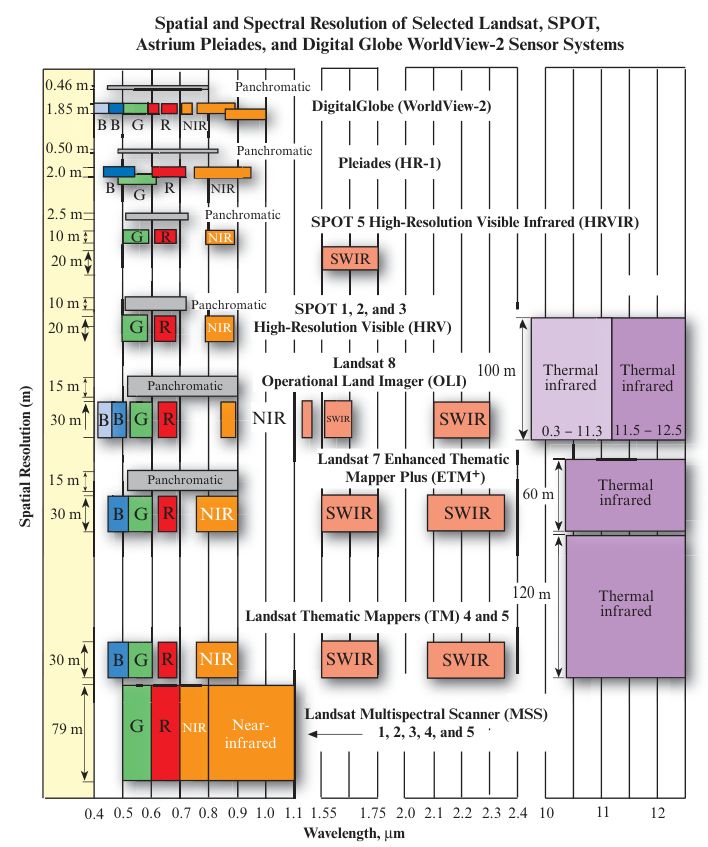
\includegraphics[width=1\textwidth]{Images/BANDAS.png}
    \end{center}
    \caption{Comparación de la distribución espectral entre los principales satélites de observación.}
    \reference{Datos tomados de \citeA{jensen2016introductory}.}
    \label{fig:BANDAS}
\end{figure}

En comparación con Sentinel-2, Landsat tiene la capacidad de obtener datos de la región térmica del espectro electromagnético, tal y como se ilustra en la Figura \ref{fig:BANDAS}. Esta característica permite recopilar información emitida directamente de la superficie terrestre. Landsat 8 cuenta con un sensor dedicado exclusivamente a esta área, el TIRS, mientras que el sensor OLI, está destinado a recopilar información de las demás regiones del espectro \cite{landsat}.

Landsat 8 ha aumentado su capacidad a aproximadamente 400 escenas diarias, superando las 250 escenas del Landsat 7 \cite{ariza2013descripcion}. Esto incrementa la probabilidad de obtener imágenes libres de nubes y aumenta la frecuencia de adquisición de datos \cite{loveland2016landsat}.

\textbf{c) Productos}

Según \citeA{ariza2013descripcion}, el formato GeoTIFF representa el estándar para la distribución de datos de Landsat, estando presente en los siguientes niveles de productos:

\begin{enumerate}
    \item \textbf{Nivel 0 (L0)}: Corresponde a las imágenes digitales crudas, sin procesar, que mantienen la secuencia de las bandas multiespectrales.

    \item \textbf{Nivel 1 Radiométrico (L1R)}: Incluye datos con correcciones radiométricas, ajustados a valores de radiancia o reflectancia espectral, derivados de datos de Nivel 0.

    \item \textbf{Nivel 1 Sistemático (L1G)}: Engloba los datos L1R con correcciones geométricas sistemáticas para el registro en una proyección cartográfica, utilizando como referencia el WGS84.

    \item \textbf{Nivel 1 Geométricamente corregido (L1Gt)}: Consiste en datos L1R con correcciones geométricas avanzadas, aprovechando información de posición a bordo y datos de control de elevación para corregir errores de paralaje.

    \item \textbf{Nivel 1 con Corrección del terreno (L1T)}: Agrupa los datos L1R con correcciones geométricas utilizando puntos de control terrestre y correcciones topográficas para contrarrestar el desplazamiento causado por el relieve.
\end{enumerate}
\subsection{Aprendizaje automático}

El aprendizaje automático es una rama de la inteligencia artificial que se centra en el desarrollo de algoritmos y modelos estadísticos que capacitan a los sistemas informáticos para mejorar su desempeño en tareas específicas mediante la experiencia adquirida a partir del procesamiento de datos \cite{elgendy2020deep}. Estos sistemas están diseñados para aprender, predecir y tomar decisiones basadas en el análisis de conjuntos extensos de datos, identificando patrones y adaptándose a nuevas situaciones sin requerir programación explícita \cite{goodfellow2016deep}.

El impacto del aprendizaje automático se extiende ampliamente en la actualidad, siendo fundamental en diversas aplicaciones como búsquedas en la web, filtrado de contenido en redes sociales y recomendaciones en plataformas de comercio electrónico \cite{geron2019hands}. Asimismo, se ha integrado en sistemas inteligentes como cámaras y dispositivos móviles, autos autónomos, vehículos aéreos no tripulados, y otros relacionados a la visión por computador \cite{patterson2017deep}.

Los algoritmos de aprendizaje automático tienen fundamentos en la estadística, en la optimización, en la teoría de la información y en la computación, y según su forma de aprender, estos pueden clasificarse en tres grupos: aprendizaje supervisado, aprendizaje no supervisado y aprendizaje por refuerzo \cite{goodfellow2016deep}.

\subsubsection{Aprendizaje supervisado}

En el aprendizaje supervisado, los algoritmos se entrenan sobre conjuntos de datos etiquetados, los cuales representan las soluciones deseadas. A estos datos se les conoce como etiquetas, lo que significa que cada ejemplo de entrenamiento está emparejado con una salida (etiqueta o valor de respuesta) \cite{geron2019hands}. El objetivo es que el algoritmo aprenda a predecir la etiqueta a partir de las características de los datos de entrada \cite{patterson2017deep}.

Tras el entrenamiento, se evalúa el algoritmo con datos no vistos durante la fase de aprendizaje para verificar su capacidad de generalización \cite{geron2019hands}. Las tareas comunes para este tipo de aprendizaje son la regresión, que busca predecir un valor numérico continuo, y la clasificación, que busca dividir los datos en subgrupos en base a sus características (ver Figura ~\ref{fig:supervised}).

\begin{figure}[H]
    \begin{center}
        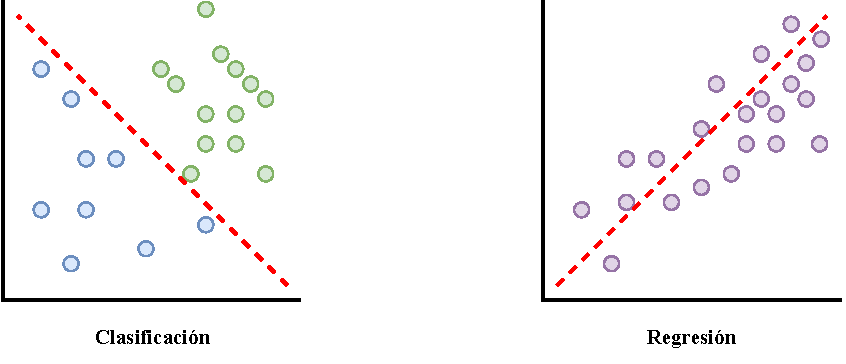
\includegraphics[width=0.9\textwidth]{Images/supervised.pdf}
    \end{center}
    \caption{Diferencias entre un problema de clasificación y un problema de regresión.}
    \reference{Elaborado por el autor.}
    \label{fig:supervised}
\end{figure}

Según \citeA{geron2019hands}, los algoritmos supervisados más importantes son: regresión lineal, regresión logística, maquina de vectores de soporte, árboles de decisión y bosques aleatorios, k vecinos cercanos y las redes neuronales.

\subsubsection{Aprendizaje no supervisado}

Los algoritmos de aprendizaje no supervisado se distinguen del aprendizaje supervisado por prescindir de conjuntos de datos etiquetados. En lugar de ello, el sistema busca comprender las estructuras y los patrones inherentes a los datos sin una orientación explícita hacia un resultado específico  \cite{geron2019hands}. Este enfoque encuentra aplicaciones en diversas tareas, como la detección de anomalías, como se observa en las máquinas de vectores de soporte de una clase; la reducción de la dimensionalidad, ejemplificada en el análisis de componentes principales; y principalmente, en el agrupamiento o clustering (ver Figura~\ref{fig:clustering}), donde se destacan métodos como K-medias, DBSCAN y análisis de conglomerados.

\begin{figure}[H]
    \begin{center}
        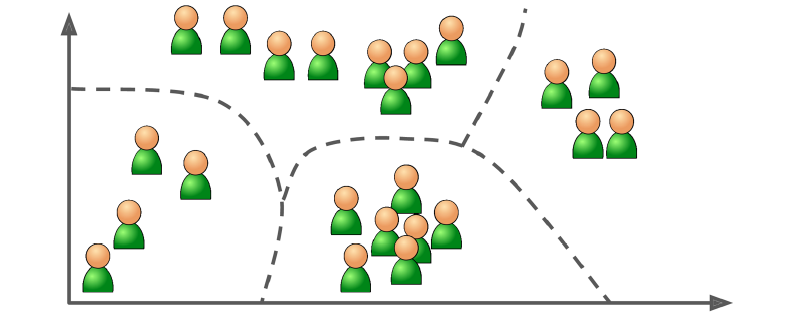
\includegraphics[width=1\textwidth]{Images/clustering.png}
    \end{center}
    \caption{Agrupamiento (clustering).}
    \reference{Datos tomados de \citeA{geron2019hands}.}
    \label{fig:clustering}
\end{figure}

\subsubsection{Aprendizaje por refuerzo}

Este tipo de aprendizaje se enfoca en la maximización de una métrica de recompensa acumulada, dictando cómo los agentes deben operar dentro de un entorno dado. A través de iteraciones de prueba y error, el agente adquiere estrategias adaptables, permitiéndole ajustar sus acciones a contextos específicos con el fin de alcanzar sus metas \cite{geron2019hands}.

\subsection{Aprendizaje profundo}

El aprendizaje profundo se basa en el uso de grandes cantidades de datos, algoritmos de optimización, funciones de activación y arquitecturas específicas para cada problema, como las redes neuronales convolucionales, las redes neuronales recurrentes y las redes generativas adversarias, por mencionar algunos \cite{geron2019hands}. Se inspira en el funcionamiento del cerebro humano y permite a las computadoras procesar datos de forma no lineal, iterativa y jerárquica, extrayendo así niveles de abstracción y representación cada vez más altos y significativos \cite{goodfellow2016deep}.

En la actualidad, es aplicado a diversos dominios como la visión por computador, el reconocimiento de voz, la traducción automática, la robótica, la biología y la medicina, y ofrece ventajas en el descubrimiento de exoplanetas, nuevos fármacos y enfermedades, estudio de la genética humana, entre otros \cite{patterson2017deep}.

Varios autores como \citeA{elgendy2020deep}, ubican al aprendizaje profundo como un subconjunto de aprendizaje automático, tal y como lo muestra la Figura \ref{fig:ia}, esto debido a que utiliza técnicas de aprendizaje supervisado, no supervisado o por refuerzo para entrenar modelos complejos y de gran capacidad.

\begin{figure}[H]
    \begin{center}
        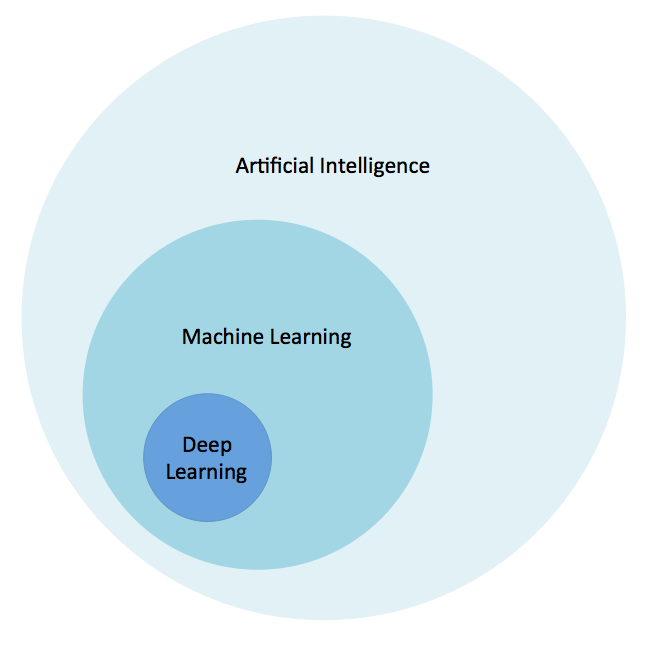
\includegraphics[width=0.6\textwidth]{Images/relation.png}
    \end{center}
    \caption{Diferencias entre inteligencia artificial (AI), aprendizaje automático (ML) y aprendizaje profundo (DL).}
    \reference{Datos tomados de \citeA{patterson2017deep}.}
    \label{fig:ia}
\end{figure}

Según \cite{patterson2017deep}, para que un algoritmo sea considerado como aprendizaje profundo debe cumplir con ciertas condiciones:

\begin{itemize} \item Mayor número de neuronas presentes que en redes anteriores. \item Formas más complejas de inter conectar neuronas y/o capas en la red. \item Extracción automática de características. \item Uso de una gran cantidad de recursos computacionales. \end{itemize}

El aprendizaje profundo se distingue por no requerir la intervención humana para extraer las características relevantes de los datos, sino que las aprende de forma automática mediante arquitecturas complejas. Estas características se usan luego para realizar tareas como clasificación, detección o generación, según se ilustra en la Figura~\ref{fig:comparasion}.

\begin{figure}[H]
    \begin{center}
        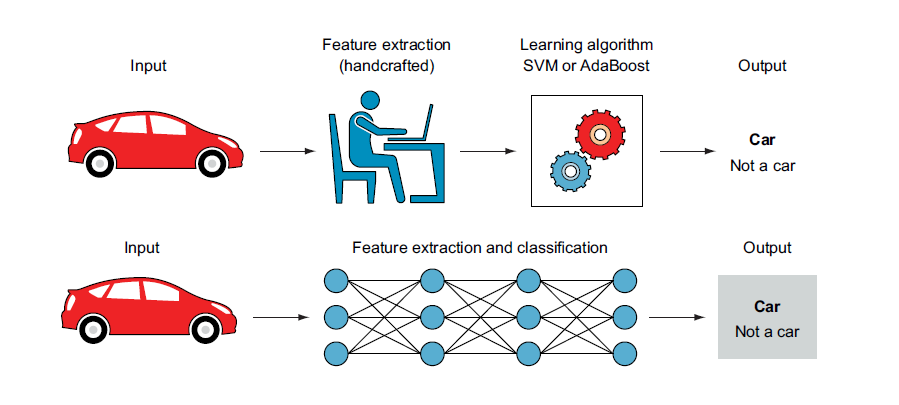
\includegraphics[width=1\textwidth]{Images/comparasion.png}
    \end{center}
    \caption{Diferencias entre el aprendizaje automático y el aprendizaje profundo.}
    \reference{Datos tomados de \citeA{elgendy2020deep}.}
    \label{fig:comparasion}
\end{figure}

Las redes neuronales son la base de los algoritmos de aprendizaje profundo. Estas redes se caracterizan por tener muchas capas que les permiten aumentar su profundidad y su capacidad de aprendizaje (de ahí el nombre ``profundo’'). Sin embargo, a mayor profundidad, mayor es el número de parámetros que se deben entrenar, lo que implica un mayor costo computacional y una mayor complejidad \cite{elgendy2020deep}.

\subsubsection{Redes neuronales artificiales (ANNs)}

Artificial Neural Networks en inglés, son algoritmos de inteligencia artificial inspirados en el funcionamiento de las neuronas biológicas, como se muestra en la Figura~\ref{fig:ComparacionNeurona} \cite{elgendy2020deep}.

\begin{figure}[H]
    \begin{center}
        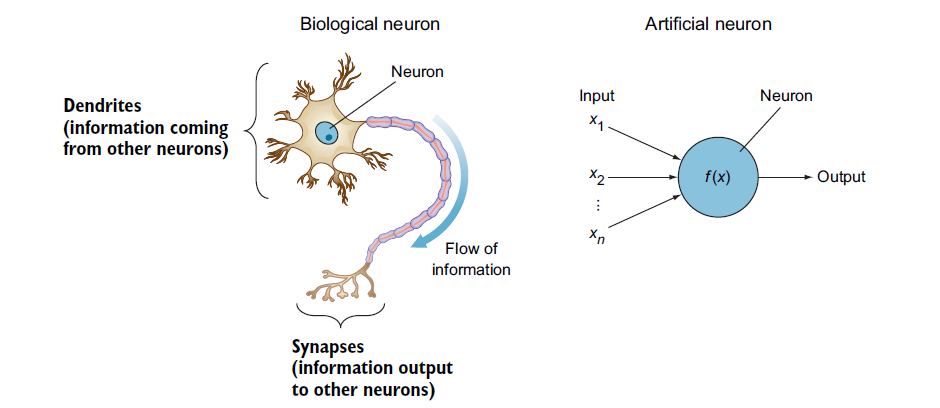
\includegraphics[width=1\textwidth]{Images/neuron.png}
    \end{center}
    \caption{Diferencias entre una neurona biológica y una neurona artificial.}
    \reference{Datos tomados de \citeA{elgendy2020deep}.}
    \label{fig:ComparacionNeurona}
\end{figure}

El perceptrón es el modelo más simple de red neuronal artificial, propuesto por Frank Rosenblatt en 1957. Se basa en una unidad de umbral lineal (LTU), que es una neurona artificial que calcula una combinación lineal de las entradas y las pesos sinápticos, y luego aplica una función de activación para obtener la salida. El perceptrón tiene una sola capa de neuronas, cada una conectada a todas las entradas del vector de características (ver Figura~\ref{fig:ann}).

\begin{figure}[H]
    \begin{center}
        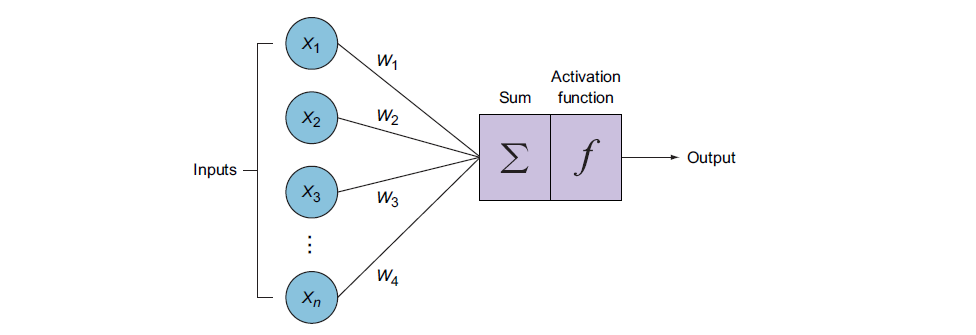
\includegraphics[width=1\textwidth]{Images/ann.png}
    \end{center}
    \caption{Arquitectura básica de una red neuronal artificial de una sola capa.}
    \reference{Datos tomados de \citeA{elgendy2020deep}.}
    \label{fig:ann}
\end{figure}

Para representar gráficamente estas conexiones, se usan neuronas especiales llamadas neuronas de entrada, que transmiten el valor que reciben. Además, se suele añadir un sesgo a cada neurona, que se modela mediante una neurona especial que siempre emite 1. El sesgo permite desplazar el umbral de activación de la neurona y mejorar su capacidad de adaptación \cite{geron2019hands}.

Cada neurona artificial recibe varias entradas y las pondera mediante unos pesos sinápticos, que son los parámetros que se ajustan mediante un algoritmo de aprendizaje basado en los resultados obtenidos. El objetivo del aprendizaje es que la red neuronal pueda aproximar una función que relacione las entradas con las salidas deseadas. Para ello, cada neurona artificial calcula una combinación lineal de las entradas y los pesos, y luego aplica una función de activación no lineal para obtener la salida \cite{patterson2017deep}. La ecuación que representa el cálculo de la salida de una neurona artificial es la siguiente:

\begin{equation} Z = f(W^T X + b) \end{equation}

Donde $Z$ es la salida de la neurona, $f$ es la función de activación, $W$ es el vector de pesos sinápticos, $X$ es el vector de entradas y $b$ es el sesgo.

\textbf{a) Perceptrón multicapa}

Es una arquitectura de red neuronal artificial que está compuesta por múltiples capas de neuronas. Cada capa puede tener más de una neurona, y estas pueden estar conectadas entre sí a través de pesos sinápticos. La arquitectura de este tipo de redes neuronales está compuesta por una capa de entrada, capas ocultas y una capa de salida \cite{geron2019hands}.

\begin{figure}[H]
    \begin{center}
        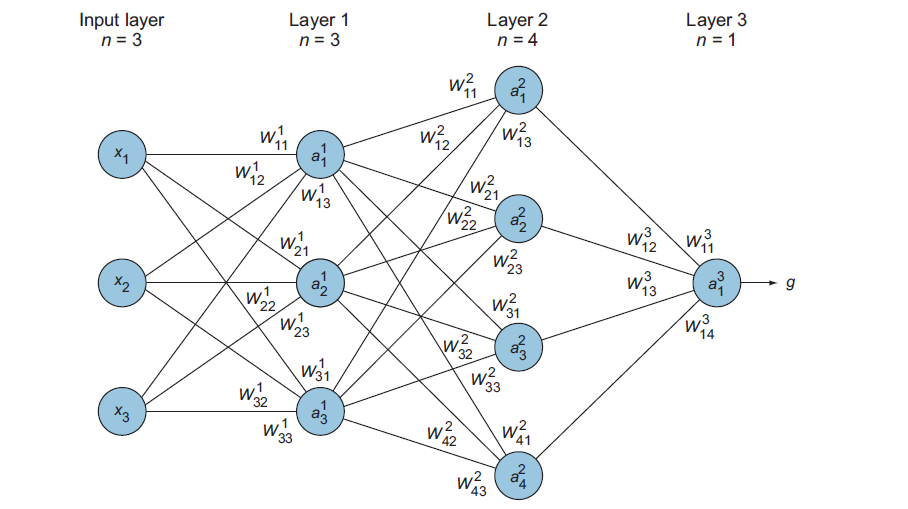
\includegraphics[width=1\textwidth]{Images/mlp.png}
    \end{center}
    \caption{Arquitectura de un perceptrón multicapa de 3 capas (1 capa de entrada, 2 capas ocultas + 1 capa de salida).}
    \reference{Datos tomados de \citeA{elgendy2020deep}.}
    \label{fig:mlp}
\end{figure}

La Figura~\ref{fig:mlp} ilustra una red neuronal artificial con entradas $X$, pesos $W$, neuronas $a$ y una salida $g$.

El proceso para obtener este último valor se llama propagación hacia adelante, y consiste en calcular la salida de cada capa de la red a partir de las entradas y los pesos, comparando la salida obtenida con la salida esperada, que se proporciona en un conjunto de datos.

Para medir la diferencia entre ambas salidas, se usa una función de error, que se busca minimizar mediante un algoritmo de optimización. Este algoritmo actualiza los pesos de la red, usando una técnica llamada propagación hacia atrás, que consiste en ajustar los pesos en sentido inverso, desde la capa de salida hasta la capa de entrada. Este ciclo se realiza hasta que la red alcance un nivel de precisión satisfactorio \cite{rashid2016make}.

\textbf{b) Funciones de activación}

Las funciones de activación buscan lograr la no linealidad de la red neuronal \cite{patterson2017deep}. Se utilizan para propagar la salida de los nodos de la capa anterior hacia la siguiente capa. Están inspiradas en el comportamiento de las neuronas biológicas, las cuales al lograr pasar un umbral emiten pulsaciones eléctricas a las demás neuronas conectadas, tratando a las neuronas que no alcancen el umbral como muertas, esto con el fin de proporcionar sólo la información relevante a la siguiente capa \cite{rashid2016make}.

Es deseable que una función de activación aproxime su función de identidad cerca al origen. La función de activación de una neurona está dada por:

\begin{equation}
    f(W^T X + b)
\end{equation}

Donde, $f$ es la función de activación, $W$ es el vector de pesos sinápticos, $X$ es el vector de entradas y $b$ es el sesgo. Usualmente, $W$ y $b$ son inicializados con valores cercanos a $0$ por el método de gradiente descendiente, por lo que $W^T X + b$ estará cerca a 0. Si $f$ aproxima su función de identidad a 0, su gradiente será aproximadamente igual a su entrada, haciendo que el algoritmo de entrenamiento converja más rápido \cite{aghdam2017guide}.

Dependiendo del tipo de gráfico que forme la función, se pueden clasificar en funciones sigmoideas (en forma de $S$), rectilíneas, por mencionar algunos.

\textbf{\textit{Sigmoidea:}} Esta determinada por la siguiente ecuación:

\begin{equation}
    f_{sigmoid}(x) = \frac{1}{1+e^{-x}}
\end{equation}

Su derivada está dada por:

\begin{equation}
    f^{'}_{sigmoid}(x) = f(x)(1-f(x))
\end{equation}

Donde, $ f_{sigmoid}(x): \mathbb{R} \rightarrow  [0,1] $.

La función sigmoidea es una función inspirada por comportamientos biológicos, por lo que fue muy usada en el diseño de redes neuronales \cite{aghdam2017guide}.

\begin{figure}[H]
    \begin{center}
        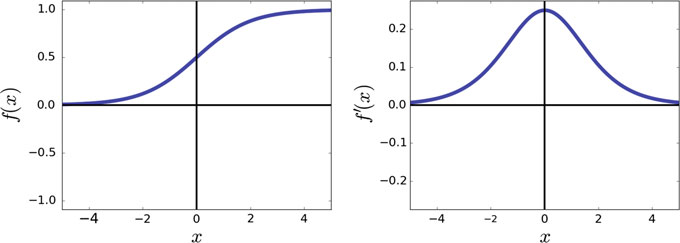
\includegraphics[width=0.7\textwidth]{Images/sigmoid.png}
    \end{center}
    \caption{Función de activación sigmoidea y su derivada correspondiente.}
    \reference{Datos tomados de \citeA{aghdam2017guide}.}
    \label{fig:sigmoid}
\end{figure}

En la Figura~\ref{fig:sigmoid} se muestra el gráfico de la función sigmoidea y su derivada.

\textbf{\textit{Tangente hiperbólica:}} Es una función re escalada de la función sigmoidea ya que su rango va desde -1 a 1 a diferencia de éste último. Esta determinada por la siguiente ecuación \cite{castaneda2019evaluation}:

\begin{equation}
    f_{tanh}(x) = \frac{e^{x}-e^{-x}}{e^{x}+e^{-x}} = \frac{1 - e^{-2x}}{1 + e^{-2x}}
\end{equation}

Su derivada está dada por:

\begin{equation}
    f^{'}_{tanh}(x) = 1 - f_{tanh}(x)^{2}
\end{equation}

Donde, $  f_{sigmoid}(x) : \mathbb{R} \rightarrow  [-1,1] $.

Además, a diferencia de la función sigmoidea, la función tangente hiperbólica aproxima su función de identidad al origen, tal y como se muestra en la Figura~\ref{fig:tangent}, esta propiedad hace posible incrementar la convergencia del algoritmo de gradiente descendiente \cite{aghdam2017guide}.

\begin{figure}[H]
    \begin{center}
        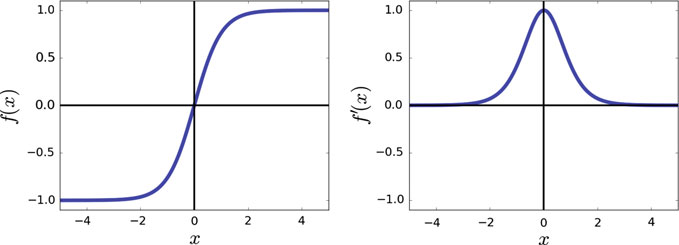
\includegraphics[width=0.7\textwidth]{Images/tangent.png}
    \end{center}
    \caption{Función de activación tangente hiperbólica y su derivada correspondiente.}
    \reference{Datos tomados de \citeA{aghdam2017guide}.}
    \label{fig:tangent}
\end{figure}

Sin embargo, esta función es propensa a caer en problemas de desvanecimiento de gradiente si la red neuronal presenta muchas capas, ya que al incrementarse el valor de $x$ la función devuelve valores saturados  \cite{aghdam2017guide}.

\textbf{\textit{Softsign:}} Esta función de activación es similar a la función tangente hiperbólica, ya que su rango también va de -1 a 1. La ecuación que representa la función es la siguiente:

\begin{equation}
    f_{softsign}(x) = \frac{x}{1 + |x|}
\end{equation}

Su derivada está dada por:

\begin{equation}
    f^{'}_{softsign}(x) = \frac{1}{(1 + |x|)^{2}}
\end{equation}

\begin{figure}[H]
    \begin{center}
        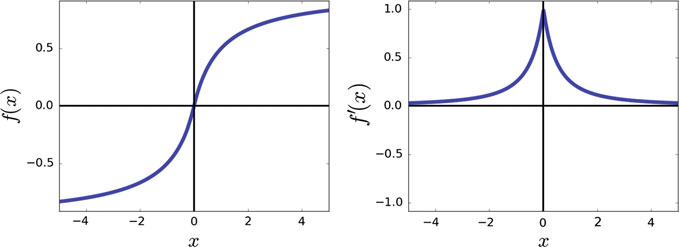
\includegraphics[width=0.7\textwidth]{Images/softsign.png}
    \end{center}
    \caption{Función de activación softsign y su derivada correspondiente.}
    \reference{Datos tomados de \citeA{aghdam2017guide}.}
    \label{fig:softsign}
\end{figure}

Como se puede observar en la Figura~\ref{fig:softsign}, la función de identidad se aproxima al origen y su derivada en este punto toma el valor de 1. Sin embargo, presenta el mismo problema de desvanecimiento de gradiente si la red neuronal presenta muchas capas, aunque en menor medida que la función de tangente hiperbólica. Además, computacionalmente requiere de menos recursos que éste último \cite{aghdam2017guide}.

\textbf{\textit{Softmax:}} Se utiliza habitualmente en la capa de salida de los clasificadores para obtener una distribución de probabilidad sobre diferentes clases. Para un vector \( \mathbf{x} \) en un espacio de \( K \) dimensiones, la función softmax se define como:

\begin{equation}
    f_{softmax}(\mathbf{x})_i = \frac{e^{x_i}}{\sum_{k=1}^{K} e^{x_k}}
\end{equation}

donde \( i = 1, \ldots, K \) y \( x_i \) representa el elemento i-ésimo del vector \( \mathbf{x} \).

La derivada de la función softmax con respecto a cada elemento \( x_i \) depende de todos los componentes del vector \( \mathbf{x} \), reflejado en la siguiente forma para la derivada parcial de \( f_{softmax}(\mathbf{x})_i \) con respecto a \( x_j \):

\begin{equation}
    \frac{\partial f_{softmax}(\mathbf{x})_i}{\partial x_j} =
    \begin{cases}
        f_{softmax}(\mathbf{x})_i \cdot (1 - f_{softmax}(\mathbf{x})_i) & \text{si } i = j,    \\
        -f_{softmax}(\mathbf{x})_i \cdot f_{softmax}(\mathbf{x})_j      & \text{si } i \neq j.
    \end{cases}
\end{equation}

Esta función es especialmente útil en problemas de clasificación multi clase y es menos propensa al problema del desvanecimiento de gradiente, especialmente cuando se utiliza en conjunto con la función de pérdida de entropía cruzada \cite{goodfellow2016deep}.

\textbf{\textit{ReLU:}} Es generalmente utilizada en redes neuronales profundas. Las funciones de activación mencionadas anteriormente tienen a desvanecer en la etapa de retro propagación cuando la red presenta muchas capas \cite{aghdam2017guide}. Una ReLU está dada por:

\begin{equation}
    f_{ReLU}(x) = max(0,x)
\end{equation}

Su derivada está dada por:

\begin{equation}
    {f}'_{ReLU}(x) = \left\{\begin{matrix}
        0 & x < 0         \\
        1 & x \geqslant 0
    \end{matrix}\right.
\end{equation}

\begin{figure}[H]
    \begin{center}
        \includegraphics[width=0.7\textwidth]{Images/relu.png}
    \end{center}
    \caption{Función de activación ReLU y su derivada correspondiente.}
    \reference{Datos tomados de \citeA{aghdam2017guide}.}
    \label{fig:relu}
\end{figure}

Esta función no lineal funciona muy bien en la práctica, su derivada cuando $ \mathbb{R}^{+}$ siempre es 1 y no se satura cuando $ \mathbb{R}^{+}$ por lo que no presenta el problema de desvanecimiento de gradiente. Esto significa que el rango de esta función de activación es $[0, \infty)$. Al no tener este problema, se considera una buena opción para entrenar redes profundas. En el caso de las neuronas muertas, esta función siempre retorna un 0 haciéndola computacionalmente más eficiente. Sin embargo, esto puede afectar el nivel de exactitud general de la red \cite{aghdam2017guide}.

\textbf{\textit{Leaky ReLU:}} Busca resolver el problema de las neuronas muestras presentes en la función ReLU. La función leaky ReLU está dada por:

\begin{equation}
    {f}_{Leaky ReLU}(x) = \left\{\begin{matrix}
        \alpha x & x < 0         \\
        x        & x \geqslant 0
    \end{matrix}\right.
\end{equation}

Y su derivada por:

\begin{equation}
    {f}'_{Leaky ReLU}(x) = \left\{\begin{matrix}
        \alpha & x < 0         \\
        1      & x \geqslant 0
    \end{matrix}\right.
\end{equation}

\begin{figure}[H]
    \begin{center}
        \includegraphics[width=0.7\textwidth]{Images/leaky-relu.png}
    \end{center}
    \caption{Función de activación Leaky ReLU y su derivada correspondiente.}
    \reference{Datos tomados de \citeA{aghdam2017guide}.}
    \label{fig:leaky-relu}
\end{figure}

Leaky ReLU asigna una pendiente a su entrada negativa (ver Figura~\ref{fig:leaky-relu}), la cual, puede tomar un valor entre [0,1] \cite{castaneda2019evaluation}. Generalmente, éste valor se establece en $ \alpha = 0.01 $. Sin embargo, según \cite{xu2015empirical}, se tiene mejor desempeño si se le asignan valores más altos al trabajar con algunos conjuntos de datos. En la práctica la función ReLU y leaky ReLU producen resultados similares, esto se debe a que las regiones positivas de ambas funciones son idénticas \cite{aghdam2017guide}.

\textbf{c) Funciones de pérdida}

Las redes neuronales utilizan funciones de pérdida para evaluar la discrepancia entre las predicciones y los valores reales. Dos de las funciones de pérdida más comunes son el Error Cuadrático Medio (MSE) y la Entropía Cruzada.

\textbf{\textit{Error Cuadrático Medio (MSE)}}: El MSE mide la diferencia cuadrática promedio entre las predicciones \(\hat{y}_i\) y las etiquetas reales \(y_i\). Su fórmula es:

\begin{equation}
    MSE(W, b) = \frac{1}{n} \sum_{i=1}^{n} (y_i - \hat{y}_i)^2
\end{equation}

Donde \(n\) es el número de ejemplos. El MSE es sensible a valores atípicos, por lo que a veces se prefiere el Error Absoluto Medio (MAE), que calcula el promedio de los valores absolutos de los errores.

\textbf{\textit{Entropía Cruzada}}: Esta función mide la diferencia entre dos distribuciones probabilísticas, como la distribución real y la predicha por la red. Su fórmula es:

\begin{equation}
    CrossEntropy(W, b) = -\frac{1}{n} \sum_{i=1}^{n} \sum_{j=1}^{m} y_{ij} \log(\hat{y}_{ij})
\end{equation}

Aquí, \(m\) es el número de clases, y \(y_{ij}\) y \(\hat{y}_{ij}\) representan la realidad y la probabilidad predicha, respectivamente.

\textbf{d) Optimización}

Para optimizar una red neuronal, se busca minimizar su función de pérdida.

\textbf{\textit{Descenso del Gradiente}}: Este método actualiza los parámetros de la red (pesos \(W\) y sesgos \(b\)) de manera iterativa para minimizar la función de pérdida.

\begin{figure}[H]
    \begin{center}
        \includegraphics[width=\textwidth]{Images/Gradiente.png}
    \end{center}
    \caption{Descenso de gradiente.}
    \label{fig:Gradiente}
    \reference{Datos tomados de \citeA{elgendy2020deep}.}
\end{figure}

Existen varias variantes del descenso de gradiente:

\begin{itemize}
    \item \textit{Descenso del Gradiente por Lotes}: Utiliza todo el conjunto de datos para cada actualización de parámetros. Es eficiente para conjuntos de datos pequeños, pero menos práctico para grandes volúmenes de datos.
    \item \textit{Descenso de Gradiente Estocástico (SGD)}: Actualiza los parámetros para cada ejemplo individual, lo que lo hace más adecuado para grandes conjuntos de datos y capaz de escapar de mínimos locales.
    \item \textit{Descenso de Gradiente Mini-Lote}: Combina los enfoques anteriores, actualizando los parámetros para un subconjunto del conjunto de datos, equilibrando eficiencia y convergencia.
\end{itemize}

La elección entre estas variantes depende del tamaño del conjunto de datos y de las características específicas del problema.

\textbf{e) Retro propagación}

La retro propagación es el proceso utilizado para calcular los gradientes necesarios para el descenso de gradiente \cite{rashid2016make}.

Durante la retro propagación, los gradientes de la función de pérdida con respecto a los pesos \(W\) y sesgos \(b\) se calculan mediante la regla de la cadena. Posteriormente, estos gradientes se utilizan para actualizar los pesos y sesgos, optimizando así el rendimiento de la red.

\textbf{\textit{Ecuaciones de retro propagación}}:

Para la última capa \(L\):

\begin{equation}
    \delta^{(L)} = \nabla_a Cost \odot \sigma'(z^{(L)})
\end{equation}

Para las capas anteriores \(l < L\):

\begin{equation}
    \delta^{(l)} = ((W^{(l+1)})^T \delta^{(l+1)}) \odot \sigma'(z^{(l)})
\end{equation}

Donde \(\delta^{(l)}\) es el vector de error para la capa \(l\), \(W^{(l+1)}\) son los pesos de la capa siguiente, \(z^{(l)}\) son las entradas a las neuronas en la capa \(l\), y \(\sigma'\) es la derivada de la función de activación.

Esta metodología asegura que cada paso del aprendizaje se enfoque en reducir la función de pérdida, guiando así a la red hacia una mejor precisión en la tarea que realiza.

\subsubsection{Redes neuronales convolucionales (CNNs)}
Son arquitecturas de redes neuronales diseñadas específicamente para procesar datos en formato de matriz bidimensional, como las imágenes. Estas estructuras de red se componen de varias capas que aplican filtros (convoluciones) a los datos de entrada para extraer características significativas \cite{geron2019hands}.

\begin{figure}[H]
    \begin{center}
        \includegraphics[width=\textwidth]{Images/ComposicionImagen.pdf}
    \end{center}
    \caption{Representación digital de una imagen.}
    \label{fig:ComposicionImagen}
    \reference{Datos tomados de \citeA{elgendy2020deep}.}
\end{figure}

Como se muestra en la Figura~\ref{fig:ComposicionImagen}, una imagen digital se representa mediante una matriz de píxeles, cada uno con un valor de intensidad asignado. Las imágenes de alta resolución presentan una entrada con alta dimensionalidad \cite{elgendy2020deep}. En redes neuronales tradicionales, cada píxel se conecta a muchas neuronas, con cada conexión representando un parámetro ajustable, resultando en un modelo con un número elevado de parámetros. Esto puede aumentar la carga computacional y propiciar el sobre ajuste \cite{rashid2016make}.

\begin{figure}[H]
    \begin{center}
        \includegraphics[width=\textwidth]{Images/VisionCNN.png}
    \end{center}
    \caption{Extracción de características de una imagen mediante el sistema visual humano.}
    \label{fig:VisionCNN}
    \reference{Datos tomados de \citeA{geron2019hands}.}
\end{figure}

Las CNNs manejan la alta dimensionalidad de las imágenes utilizando filtros convolucionales para procesar la matriz de píxeles, reduciendo así la dimensionalidad de los datos y extrayendo automáticamente características clave como bordes, texturas y colores. Este proceso es análogo a cómo el sistema visual humano interpreta información visual, ilustrado en la Figura~\ref{fig:VisionCNN}. Esto conduce a una reducción en el número de parámetros y la complejidad computacional, aumentando la eficiencia y evitando el sobre ajuste \cite{geron2019hands}.

La arquitectura fundamental de una CNN se muestra en la Figura~\ref{fig:ArquitecturaCNN}.

\begin{figure}[H]
    \begin{center}
        \includegraphics[width=\textwidth]{Images/ArquitecturaCNN.png}
    \end{center}
    \caption{Arquitectura base de una red neuronal convolucional.}
    \label{fig:ArquitecturaCNN}
    \reference{Datos tomados de \citeA{elgendy2020deep}.}
\end{figure}

Dentro de la arquitectura de una CNN, se encuentra el extractor de características, que incluye capas convolucionales y de agrupación (pooling). Las capas convolucionales identifican patrones locales en imágenes, como bordes o texturas, mientras que el agrupamiento reduce la dimensionalidad espacial, conservando las características más destacadas. La clasificación se realiza en las capas totalmente conectadas, que usan un vector de características aplanado para calcular las probabilidades de cada clase. Finalmente, la capa de salida produce predicciones probabilísticas de clases, ofreciendo una interpretación numérica de la probabilidad de que una imagen pertenezca a una clase específica \cite{elgendy2020deep}.

\textbf{a) Capas de entrada y salida}

La capa de entrada en una CNN consiste en las imágenes a procesar, representadas como matrices numéricas correspondientes a los valores de píxeles en canales de color, comúnmente rojo, verde y azul (RGB). Esta capa prepara las imágenes para su procesamiento en la red, estandarizando sus dimensiones para adecuarse a la arquitectura de la red \cite{rashid2016make, geron2019hands}.

La capa de salida en una CNN está orientada a proporcionar los resultados del proceso de clasificación. Para la clasificación de imágenes, esta capa suele emplear una función de activación softmax, generando un vector de probabilidades. Cada elemento de este vector indica la probabilidad de que la imagen corresponda a una de las clases predefinidas. La dimensión de esta capa es igual al número de clases que el modelo está capacitado para identificar \cite{geron2019hands}.

\textbf{b) Capas convolucionales}

Las capas convolucionales en una red neuronal convolucional utilizan filtros o kernels que se desplazan a través de la entrada para generar mapas de características, detectando patrones locales como texturas y bordes. La configuración de estos filtros influye en las características que se extraen \cite{rashid2016make, geron2019hands}.

\textbf{\textit{Convolución:}} Durante la convolución, un filtro se aplica sobre la imagen de entrada, desplazándose y realizando operaciones matemáticas para producir un valor en el mapa de características \cite{aghdam2017guide}.

\begin{figure}[H]
    \begin{center}
        \includegraphics[width=\textwidth]{Images/CapaConvolucion.png}
    \end{center}
    \caption{Proceso de convolución en una red neuronal convolucional.}
    \label{fig:CapaConvolucion}
    \reference{Datos tomados de \citeA{elgendy2020deep}.}
\end{figure}

\textbf{\textit{Stride:}} El stride define el desplazamiento del filtro a lo largo de la entrada. Un stride mayor implica saltos más grandes del filtro, resultando en un mapa de características de menor tamaño. La fórmula para calcular el tamaño de salida sin considerar el padding es:

\begin{equation}
    \label{ecu:conv_stride_sin_padding}
    n_{salida} = \left[ \frac{n_{entrada} - n_{filtro}}{stride} + 1 \right]
\end{equation}

Donde \( n_{entrada} \) es el tamaño de la entrada y \( n_{filtro} \) el tamaño del filtro.

\textbf{\textit{Padding:}} El padding se utiliza para añadir bordes adicionales a la entrada, permitiendo que el filtro se aplique por completo incluso en los bordes, y manteniendo así el tamaño original de la imagen. Con padding, la fórmula para calcular el tamaño de salida se ajusta a:

\begin{equation}
    \label{ecu:conv_stride_con_padding}
    n_{salida} = \left[ \frac{n_{entrada} - n_{filtro} + 2 \times padding}{stride} + 1 \right]
\end{equation}

Donde \( padding \) representa el número de píxeles agregados alrededor de la entrada.

\textbf{\textit{Funciones de Activación Intermedias:}} Tras la convolución, las funciones de activación, como ReLU (Rectified Linear Unit), se aplican a los vectores de características para introducir no linealidades, permitiendo a la red aprender y representar datos más complejos. La función ReLU se define como:

\begin{equation}
    \label{ecu:relu}
    ReLU(x) = max(0, x)
\end{equation}

Donde \( x \) es el valor de entrada a la función de activación.

\textbf{c) Capas de agrupación (Pooling)}

Buscan reducir las dimensiones espaciales de las entradas sin alterar su profundidad. Esta técnica, al disminuir la cantidad total de datos, mejora la eficiencia computacional y reduce el número de parámetros del modelo, lo que ayuda a prevenir el sobre ajuste. Además, proporciona invariancia a traslaciones, mejorando la habilidad del modelo para reconocer patrones independientemente de su ubicación en la imagen \cite{geron2019hands, patterson2017deep}.

El proceso de agrupación emplea un kernel de pooling que se desplaza sobre la entrada con un stride específico. El tipo más común es el max pooling, que selecciona el valor máximo dentro del área cubierta por el kernel (ver Figura~\ref{fig:2-pooling}). Sin embargo, existen otros tipos de pooling, como el average pooling y el stochastic pooling, cada uno con sus propias características y aplicaciones \cite{scherer2010evaluation, zeiler2013stochastic}.

La ecuación para calcular el tamaño de salida de una capa de agrupación es la siguiente:

\begin{equation}
    \label{ecu:pooling_output}
    n_{salida} = \left[ \frac{n_{entrada} - n_{kernel} + 2 \times padding}{stride} + 1 \right]
\end{equation}

Donde \( n_{entrada} \) es el tamaño de la entrada, \( n_{kernel} \) es el tamaño del kernel de pooling, \( padding \) es el número de píxeles agregados alrededor de la entrada, y \( stride \) es el desplazamiento del kernel.

\begin{figure}[H]
    \begin{center}
        \includegraphics[width=\textwidth]{Images/2-pooling.png}
    \end{center}
    \caption{Ilustración del proceso de agrupación en una red neuronal convolucional usando un kernel de pooling.}
    \label{fig:2-pooling}
\end{figure}

Esta técnica se aplica a cada uno de los mapas de características generados por las capas convolucionales previas, reduciendo efectivamente las dimensiones espaciales mientras se mantiene la profundidad de la entrada \cite{geron2019hands}.

\textbf{e) Arquitecturas}

La arquitectura inicial de las redes neuronales convolucionales (CNN) se remonta a 1995 con la introducción de LeNet. Diseñado por Yann LeCun, este modelo fue pionero en incorporar capas convolucionales para el procesamiento de imágenes \cite{lecun1998gradient}. En los años siguientes, las CNN han experimentado avances significativos, especialmente en el campo de la visión por computadora. Un hito en este desarrollo fue la presentación de AlexNet en 2012 \cite{krizhevsky2012imagenet}, una arquitectura que demostró una mejora sustancial en la precisión de las tareas de clasificación de imágenes en el desafío ImageNet, impulsando así un renovado interés y avance en la investigación en este tipo de redes neuronales \cite{alom2018history}.

Los avances en el campo de las redes neuronales convolucionales han propiciado el desarrollo de diversas arquitecturas especializadas, adaptadas a tareas específicas de procesamiento de imágenes \cite{alom2018history}. En la detección de objetos, modelos como VGG-16, YOLO, Fast R-CNN, Faster R-CNN y ResNet han demostrado ser eficaces. Paralelamente, en la segmentación de objetos, se han empleado con éxito arquitecturas como U-Net, Mask R-CNN, SegNet y DeepLab v3+, abordando desde la segmentación semántica hasta la segmentación por instancia \cite{hoeser2020object, hoeser2020object2}.

En el Cuadro~\ref{tab:ArquitecturasCnn} se presentan las características principales de las arquitecturas de redes neuronales convolucionales más relevantes para la segmentación de objetos.

\begin{table}[H]
    \caption{Arquitecturas de redes neuronales convolucionales para la segmentación de objetos}
    \small
    \begin{tabularx}{\textwidth}{llp{2.5cm}X}
        \hline
        \textbf{Año} & \textbf{Nombre}       & \textbf{Creador}                 & \textbf{Descripción}                                                                                                                                                                                                                                                                                                                                                                                                                                                         \\
        \hline
        2015         & U-Net                 & \citeA{ronneberger2015u}         & Diseño codificador-decodificador enfocado en la segmentación semántica a nivel de píxel. Utiliza capas convolucionales y max-pooling para reducir la dimensionalidad espacial y profundizar en características. Su decodificador emplea up-sampling y convoluciones para reconstruir la resolución espacial, junto con conexiones de salto que concatenan características del codificador y decodificador, facilitando la precisión en la localización de bordes y detalles. \\
        \hline
        2017         & SegNet                & \citeA{badrinarayanan2017segnet} & Arquitectura codificador-decodificador optimizada para la eficiencia de memoria y cómputo. Combina capas convolucionales y max-pooling para la extracción de características, seguidas por up-sampling en el decodificador. Reutiliza índices de pooling para minimizar parámetros y uso de memoria, adecuada para aplicaciones en tiempo real y con recursos limitados.                                                                                                     \\
        \hline
        2017         & {Mask \newline R-CNN} & \citeA{he2017mask}               & Basada en Faster R-CNN, opera en dos fases: propone regiones de interés y luego, para cada región, clasifica el objeto, predice su cuadro delimitador y genera una máscara de segmentación a nivel de píxel.                                                                                                                                                                                                                                                                 \\
        \hline
        2018         & DeepLabv3+            & \citeA{chen2018encoder}          & DeepLabv3+ integra una red backbone (Xception o MobileNet) con un módulo ASPP para abordar escalas múltiples. Incluye un módulo decodificador que refina los detalles de segmentación, especialmente en bordes. Utiliza convoluciones atrous para capturar información contextual eficientemente.                                                                                                                                                                            \\
        \hline
        2019         & YOLACT                & \citeA{bolya2019yolact}          & YOLACT emplea una red backbone (como ResNet-50 o ResNet-101) para extracción de características. Cuenta con una cabeza de detección de instancias con cinco ramas: clasificación, caja delimitadora, coeficientes de máscara, prototipos de máscara, y selección de instancias. Realiza segmentación de instancias basada en coeficientes para desacoplar la máscara y detección de cajas.                                                                                   \\
        \hline
    \end{tabularx}
    \begin{minipage}{\textwidth}
        \vspace{10pt}
        \reference{Elaborado por el autor.}
        \label{tab:ArquitecturasCnn}
    \end{minipage}
\end{table}

\subsubsection{Redes generativas adversarias (GANs)}

Las redes neuronales de confrontación generativa (en inglés, Generative Adversarial Networks, abreviado como GANs) fueron introducidas por Ian Goodfellow en 2014 \cite{goodfellow2014generative}. Estas redes se basan en la interacción de dos sub modelos distintos: un modelo generativo y un modelo discriminatorio, como se ilustra en la Figura~\ref{fig:GANs}. El modelo discriminatorio se encarga de determinar si una muestra pertenece al conjunto de datos real o ha sido generada artificialmente. Por otro lado, el modelo generativo tiene como objetivo producir muestras que imiten fielmente la distribución de datos original.

\begin{figure}[H]
    \begin{center}
        \includegraphics[width=1\textwidth]{Images/gans.png}
    \end{center}
    \caption{Arquitectura general de una red generativa adversaria.}
    \reference{Datos tomados de \citeA{elgendy2020deep}.}
    \label{fig:GANs}
\end{figure}

El entrenamiento del discriminador implica maximizar la probabilidad de asignar etiquetas correctas tanto a las muestras reales del conjunto de entrenamiento como a las generadas por el generador. De forma paralela, el entrenamiento del generador se enfoca en minimizar la expresión \(\log(1 - D(G(z)))\). En este contexto, la función objetivo óptima para el equilibrio entre el generador y el discriminador se define mediante un juego minimax con una función de valor \(V(G, D)\) dada por:

\begin{equation}
    \underset{G}{min}\:\underset{D}{max}\: \mathbb{E}_{x \sim p_{x}(x)}[\log D(x)] + \mathbb{E}_{z \sim p_{z}(z)} [\log (1-D(G(z)))]
\end{equation}

El análisis teórico de las GANs sugiere que su criterio de entrenamiento puede permitir la recuperación de la distribución de los datos generados. Sin embargo, en la práctica, esta optimización se lleva a cabo mediante un enfoque iterativo y numérico. Según la ecuación previamente mencionada, la optimización de \(D\) en cada ciclo de entrenamiento resultaría computacionalmente inviable y podría causar overfitting en conjuntos de entrenamiento de tamaño limitado \cite{jiang2018deep}.

Para mitigar la inestabilidad durante el entrenamiento de las GANs, se han desarrollado variantes como las GANs de Wasserstein. Estas versiones buscan ofrecer una mayor estabilidad en el proceso de entrenamiento. Se ha observado que el método de Wasserstein converge más rápidamente y produce muestras de mayor calidad en comparación con las GANs tradicionales \cite{arjovsky2017wasserstein}. Actualmente, este tipo de redes neuronales encuentra aplicaciones en diversas áreas, incluyendo transferencia de estilo, generación de imágenes a partir de características condensadas y creación de sonidos, por mencionar algunas \cite{goodfellow2016deep}.


\chapter{METODOLOGÍA}
\label{chp:Metodologia}
\thispagestyle{fancy} % Aplica el estilo de página a la primera página del capítulo.

\section{Tipo y diseño de la investigación}
\label{sec:TipoDisenoInvestigacion}

\subsection{Tipo de investigación}

La presente investigación se clasifica como cuantitativa y aplicada. La investigación cuantitativa se distingue por el énfasis en la recolección y análisis de datos numéricos, así como su interpretación a través de técnicas estadísticas \cite{kothari2004research, creswell2017research}. Este estudio emplea algoritmos de aprendizaje profundo, los cuales se entrenan y validan con datos numéricos, es decir, los píxeles de las imágenes satelitales y sus correspondientes etiquetas semánticas. Esta estrategia permite un análisis cuantitativo detallado y una evaluación objetiva del rendimiento del modelo de segmentación semántica propuesto.

Además, la investigación se caracteriza como aplicada. A diferencia de la investigación básica, la cual se orienta hacia la comprensión fundamental de los fenómenos, la investigación aplicada tiene como objetivo principal resolver problemas prácticos específicos mediante la aplicación de conocimientos científicos \cite{kothari2004research}. En este caso, el problema que se resuelve es el de mejorar la efectividad del mapeo semiautomático de glaciares limpios y cubiertos en imágenes satelitales.

\subsection{Diseño de la investigación}

En cuanto al diseño de la investigación, el estudio se fundamenta en un diseño experimental. Los diseños experimentales involucran la manipulación de una o más variables independientes para observar su efecto en una variable dependiente, mientras se controlan las demás variables \cite{marczyk2010essentials}. En este estudio, las variables independientes son los parámetros del modelo de segmentación semántica basado en aprendizaje profundo y la variable dependiente es el la efectividad del mapeo de glaciares limpios y cubiertos en imágenes satelitales. Este diseño permite establecer relaciones causales entre las variables y ofrece un mayor control sobre el proceso de investigación.

\section{Unidad de análisis}
\label{sec:UnidadAnalisis}

En la presente investigación, la unidad de análisis está constituida por los glaciares limpios y cubiertos presentes en imágenes satelitales.

\section{Población de Estudio}
\label{sec:PoblacionEstudio}

La población de estudio para esta investigación está compuesta por el conjunto total de imágenes satelitales que exhiben cobertura glaciar (específicamente, glaciares tropicales), las cuales son capturadas a través de sensores remotos satelitales.

\section{Tamaño de muestra}
\label{sec:TamanoMuestra}

El tamaño de la muestra para esta investigación se determina mediante la selección de imágenes satelitales que cumplen con criterios definidos. Estos criterios se centran en la presencia de cobertura glaciar, específicamente glaciares tropicales, ya sean limpios o cubiertos, y que estén ubicados en las regiones de la Cordillera Blanca y la Cordillera Vilcabamba en Perú.

\section{Selección de muestra}
\label{sec:SeleccionMuestra}

En el contexto de la presente investigación, se adoptó un enfoque de muestreo no probabilístico aplicado a una población finita específica. Este enfoque combinó técnicas de muestreo por conveniencia y muestreo por juicio de expertos.

El muestreo por conveniencia tuvo lugar al seleccionar el área de estudio, lo cual se debió principalmente a la disponibilidad de datos ya establecidos en el Inventario de Glaciares de Perú. Este inventario fue llevado a cabo en 2018 por el Instituto Nacional de Investigación en Glaciares y Ecosistemas de Montaña. Se encontró que se contaba con información de primera mano, validada y aprobada por la entidad encargada del análisis de ecosistemas de montaña en Perú. Gracias a esto, se pudo obtener la información vectorial correspondiente a la delimitación de glaciares limpios y cubiertos. Esta información resultó de vital importancia, ya que posibilitó la creación automatizada de "máscaras", un paso clave para el entrenamiento de los modelos de segmentación semántica.

Además, se disponía de información acerca del proceso metodológico empleado para la realización de dicho inventario, lo que permitió obtener detalles sobre la metodología utilizada, las características geológicas y morfológicas de cada cordillera con presencia glaciar, información histórica estructurada e información utilizada para el proceso de identificación, incluyendo una lista de las imágenes satelitáles utilizadas, modelos digitales de elevación, imágenes de radar, imágenes de alta resolución, el software utilizado y el proceso de recopilación de resultados.

Por otro lado, se utilizó el muestreo por juicio de expertos, el cual se basó en la elección de imágenes satelitales mediante la experiencia y conocimiento de especialistas en glaciología y teledetección que participaron en el inventario de glaciares previamente mencionado. Estos expertos aportaron su juicio y criterio para seleccionar las imágenes más adecuadas, considerando los siguientes factores:

\begin{enumerate} 
    \item Imágenes satelitales obtenidas durante el periodo comprendido entre los meses de julio y noviembre.
    \item Porcentaje de nubosidad menor al 10\%.
    \item Escasa o nula cobertura de nieve temporal.
    \item Año base 2016.
\end{enumerate}

El primer criterio se alinea con el tercer criterio, ya que se aplica durante los meses de temporada seca. Durante este período, la nieve estacional es claramente identificable, lo que facilita su distinción de la nieve glaciar \cite{reserva2021}. Según \citeA{inaigem2017manual}, se considera de gran importancia utilizar imágenes satelitales multiespectrales con un bajo porcentaje de nubosidad (menor al 10\%). Esto con el objetivo de obtener una mayor información espectral de los glaciares, evitando interferencias que pudieran resultar en posibles errores en la identificación. Finalmente, el año base (2016) corresponde al año en el cual se llevó a cabo el proceso de identificación y clasificación de los glaciares presentes en el Inventario Nacional de Glaciares de Perú publicado en el año 2018.

Aunque en la presente investigación predominó el uso de imágenes satelitales multiespectrales, adicionalmente se emplearon modelos digitales de elevación con una resolución espacial de 12.5 metros, extraídos de las imágenes proporcionadas por el satélite ALOS-PALSAR, los cuales facilitaron la generación de diversos productos, incluyendo curvas de nivel, modelos de sombreado, así como mapas de orientación y pendiente.

\section{Técnicas de recolección de datos}
\label{sec:TecnicaRecoleccionDatos}

El Cuadro~\ref{tab:TecnicasInstrumentosRecoleccionDatos} detalla las técnicas e instrumentos de recolección de datos utilizados en la presente investigación:

\begin{table}
\caption{Técnicas e instrumentos de recolección de datos}
\small
\begin{tabularx}{1\textwidth}{XX} 
\hline
\textbf{Técnica} & \textbf{Instrumento} \\ \hline
    \textbf{Documentos y registros}: Se usaron fuentes como documentos oficiales, libros, artículos científicos y estudios de revisiones sistemáticas. Esto con el objetivo de respaldar el marco teórico y aclarar los conceptos importantes para la investigación actual. Esta recolección de datos se realizó mediante una metodología basada en criterios de selección definidos. & \textbf{Bases de datos bibliográficas}: Se emplearon múltiples bases de datos bibliográficas para realizar la recopilación de antecedentes de la investigación y de trabajos relacionados, tal y como se especifica en \ref{suc:RevisionSistematicaLiteratura}. \newline \textbf{Bibliotecas digitales}: Se hizo uso de múltiples bibliotecas digitales para la recopilación de libros, artículos e informes relacionados a la presente investigación. \newline  \textbf{Archivos institucionales}: Se obtuvo información de archivos institucionales, principalmente de informes de inventarios glaciares de países de la región. \newline  \textbf{Gestores de referencias}: Si hizo uso de gestores de referencias como \href{https://www.zotero.org/}{Zotero} y \href{https://www.mendeley.com/}{Mendeley}. De igual manera, se emplearon herramientas de gestión para efectuar la revisión sistemática de la literatura, tal como \href{https://parsif.al/}{Parsifal}.\\ \hline
\textbf{Técnicas digitales}: Se recopiló información por medio de herramientas en línea. Esta información incluyó archivos, imágenes, vídeos, conjuntos de datos, información vectorial, imágenes satelitales, modelos digitales de elevación, y datos históricos esquematizados. & \textbf{Fichas de descarga}: Toda la información primaria adquirida a través de internet se documentó en una ficha de descarga. Esta ficha incluyó detalles como la fuente de la información, el contenido del archivo y la fecha de adquisición. \\ \hline
\textbf{Experimentos}: Se extrajo información de los experimentos ejecutados, los cuales se fundamentaron en métricas predefinidas. Este proceso implicó la adquisición de estas métricas, documentación de resultados y el seguimiento de hiperparámetros durante las etapas de entrenamiento, evaluación y pruebas del modelo. & \textbf{Registro de pruebas}: Se utilizó un registro de pruebas que documentó los hiperparámetros establecidos para cada modelo, junto con los resultados adquiridos en las fases de entrenamiento, evaluación y pruebas del modelo. \newline \textbf{Herramientas de gestión de experimentos}: Se utilizó una herramienta digital llamada \href{https://wandb.ai/}{Wandb} para la gestión de experimentos. Esta permitió organizar las ejecuciones, preservar los resultados obtenidos y los hiperparámetros establecidos. Cabe destacar que esta herramienta fue compatible únicamente con modelos programados en Python, a diferencia del registro de pruebas.
\\  \hline
\end{tabularx}
\begin{minipage}{\textwidth}
    \vspace{10pt}
    \reference{Elaborado por el autor.}
    \label{tab:TecnicasInstrumentosRecoleccionDatos}
\end{minipage}
\end{table}

\section{Análisis e interpretación de la información}
\label{sec:AnalisisInterpretacionInformacion}

Una vez finalizada la fase de recolección de datos, se dio inicio al análisis e interpretación de la información. Se utilizaron todos los documentos bibliográficos disponibles para respaldar el marco teórico de la investigación. En relación a los datos recopilados para los experimentos, se siguió un proceso metodológico que abarcó las siguientes etapas:

\begin{enumerate}
    \item Preprocesamiento.
    \item Entrenamiento, validación y pruebas.
    \item Posprocesamiento.
    \item Evaluación de resultados.
\end{enumerate}

\subsection{Preprocesamiento}

En esta etapa, se normalizó la información recolectada de diversas fuentes, tanto para datos vectoriales como para datos raster. En el caso de los datos vectoriales, se implementó un proceso de rasterización para crear máscaras a partir de la información de los glaciares delimitados, manteniendo la clasificación entre glaciar limpio y glaciar cubierto. Previo a esto, se estandarizó el sistema de coordenadas empleado, de manera que todos los productos cartográficos se ajustaran a \textit{EPSG:32717 - WGS 84 / UTM zone 17S}, con el objetivo de prevenir problemas asociados a un manejo incorrecto.

Posteriormente, se efectuó la estandarización de la resolución espacial de todas las imágenes multiespectrales y los productos derivados de los modelos digitales de elevación. Por último, se procedió a la selección de canales de entrada para el modelo de segmentación semántica, que incluían las bandas espectrales de las imágenes Sentinel-2, los productos derivados de los modelos digitales de elevación e índices espectrales como NDSI, NDWI y NDVI.

\subsection{Entrenamiento y validación}

La etapa de entrenamiento y validación inició con la creación de mosaicos de 256x256 derivados de las imágenes multibanda y sus máscaras asociadas correspondientes a la Cordillera Blanca. Dada la limitada cantidad de mosaicos disponibles, se decidió implementar un proceso de aumento de datos para incrementar la cantidad de mosaicos empleados en la fase de entrenamiento y validación. Posteriormente, se procedió a configurar los hiperparámetros de los distintos modelos a utilizar, incluyendo el modelo propuesto en la investigación. Se buscó utilizar los mismos hiperparámetros en todos los modelos con el objetivo de establecer una comparación equitativa y objetiva de su rendimiento.

En la configuración de cada modelo, se dividió el conjunto de datos en una proporción del 80\% para entrenamiento y un 20\% para validación. Durante cada proceso de entrenamiento, se definieron las métricas utilizadas para evaluar los resultados. Dichas métricas y los hiperparámetros empleados se documentaron utilizando herramientas como Wandb, que facilitaron el seguimiento y trazabilidad de la ejecución de los experimentos. En caso de incompatibilidad de algún modelo con dicha herramienta, se recurrió a un registro de pruebas para almacenar la información pertinente.

Finalmente, se recogieron los resultados del proceso de entrenamiento y validación, así como el archivo de pesos correspondiente a la época de mayor precisión en el conjunto de datos de validación.
 
\subsection{Posprocesamiento}

Una vez que se entrenaron los modelos de segmentación semántica, se utilizó el archivo de pesos correspondiente para llevar a cabo la segmentación de las imágenes multibanda de la Cordillera Vilcabamba. A diferencia de las imágenes de la Cordillera Blanca, estas no se emplearon para la generación de mosaicos hasta este punto. Sin embargo, debido a la arquitectura del modelo, en esta etapa del proceso se generaron mosaicos en formato TIFF de 256x256, conservando la información de posicionamiento, sin la necesidad de realizar ninguna técnica de aumento de datos.

A continuación, se procedió a realizar la segmentación utilizando el archivo de pesos mencionado anteriormente, el cual contenía los parámetros de la red neuronal en la época con la mejor precisión obtenida. Una vez generadas las máscaras segmentadas por la red, se utilizó la información de posicionamiento almacenada para cada mosaico, permitiendo la reconstrucción de la forma de la imagen original con los valores segmentados por el modelo de segmentación.

Finalmente, se llevó a cabo la vectorización de los resultados. Dado que la imagen segmentada conservaba la información de glaciares limpios y cubiertos en forma de valores de píxeles, fue posible generar los dos tipos de polígonos requeridos para la evaluación de resultados.

\subsection{Evaluación de resultados}

Se llevaron a cabo dos tipos de evaluaciones de los resultados obtenidos. La primera se basó en las métricas conseguidas durante el proceso de entrenamiento y validación de los modelos. Estas métricas incluyeron: Overall Accuracy, Precisión, Recall, F1-Score, Coeficiente de Dice y, principalmente, Intersection Over Union (IoU). La evaluación de estos resultados se realizó a través de tablas resumen que compararon las métricas obtenidas entre los diferentes experimentos realizados.

Por otro lado, se efectuó una comparación de los resultados alcanzados tras el posprocesamiento con las imágenes destinadas para las pruebas, específicamente las imágenes de la Cordillera Vilcabamba. Además, se llevó a cabo una comparación a nivel de datos vectoriales para determinar el error en términos de distancia en $km^2$ entre los polígonos de segmentación correspondientes al inventario y los polígonos generados por los modelos de segmentación semántica, incluyendo el modelo propuesto en la presente tesis.

\chapter{PROPUESTA}
\label{chp:Propuesta}
\thispagestyle{fancy} % Aplica el estilo de página a la primera página del capítulo.

 
La realización de un estudio glaciológico implica la ejecución de diversas etapas consecutivas, que abarcan una serie de tareas tanto en gabinete como en campo. Las tareas en gabinete comprenden el análisis bibliográfico inicial, la adquisición de datos históricos, la exploración de enfoques previos y, de manera predominante, el análisis de la información compilada para la creación de modelos \cite{ermolin2015ambientes}. Esta información recopilada puede ser obtenida en el campo a través de visitas y recolección de muestras. Sin embargo, debido a la alta complejidad asociada con el acceso a los glaciares, se han incorporado otras técnicas como la adquisición de datos de manera remota mediante teledetección.

\section{Obtención de datos}


En el siguiente cuadro se listan las imágenes Sentinel-2 utilizadas correspondientes a la Cordillera Blanca:

\begin{table}[H]
   \centering
   \caption{Listado de imágenes satelitales}
   \label{tab:listado-imagenes-satelitales-blanca}
   \begin{tabularx}{1\textwidth}{cXcc} 
\hline
\textbf{Fecha} & \textbf{Identificador} & \textbf{Resolución espacial (m)} & \textbf{Nivel} \\
\hline
28/07/2016 & S2A\_OPER\_MSI\_L1C\_TL\_MTI\_\_2016
0728T215553\_A005742\_T17 & 10 - 20 - 60 & L1C \\
15/11/2016 & S2A\_OPER\_MSI\_L1C\_TL\_SGS\_\_2016
1115T202633\_A007315\_T17 & 10 - 20 - 60 & L1C \\
28/07/2016 & S2A\_OPER\_MSI\_L1C\_TL\_MTI\_\_2016
0728T215553\_A005742\_T18 & 10 - 20 - 60 & L1C \\
15/11/2016 & S2A\_OPER\_MSI\_L1C\_TL\_MTI\_\_2016
1115T215249\_A007315\_T18 & 10 - 20 - 60 & L1C \\
\hline
\end{tabularx}
\end{table}

En el siguiente cuadro se listan las imágenes Sentinel-2 utilizadas correspondientes a la Cordillera Vilcabamba:

\begin{table}[H]
   \centering
   \caption{Listado de imágenes satelitales}
   \label{tab:listado-imagenes-satelitales-vilcabamba}
   \begin{tabularx}{1\textwidth}{cXcc} 
\hline
\textbf{Fecha} & \textbf{Identificador} & \textbf{Resolución espacial (m)} & \textbf{Nivel} \\
\hline
28/07/2016 & S2A\_OPER\_MSI\_L1C\_TL\_MTI\_\_2016
0728T215553\_A005742\_T17 & 10 - 20 - 60 & L1C \\
15/11/2016 & S2A\_OPER\_MSI\_L1C\_TL\_SGS\_\_2016
1115T202633\_A007315\_T17 & 10 - 20 - 60 & L1C \\
28/07/2016 & S2A\_OPER\_MSI\_L1C\_TL\_MTI\_\_2016
0728T215553\_A005742\_T18 & 10 - 20 - 60 & L1C \\
15/11/2016 & S2A\_OPER\_MSI\_L1C\_TL\_MTI\_\_2016
1115T215249\_A007315\_T18 & 10 - 20 - 60 & L1C \\
\hline
\end{tabularx}
\end{table}

\subsection{Descarga de imágenes SENTINEL-2}

\subsubsection{Cordillera Blanca}

\subsubsection{Cordillera Vilcabamba}

Se incorporó una imagen adicional al inventario de glaciares tras la identificación de una porción limitada del área que no estaba cubierta por las imágenes satelitales previamente definidas.

\begin{figure}[H]
   \centering
   \includegraphics[width=1\textwidth]{Images/imagen_geometria_adicional.png}
   \label{fig:gan1}
   \caption[Escasez de cobertura glaciar en la cordillera Vilcabamba según imágenes satelitales encontradas y el inventario de glaciares del Perú de 2018.]{Escasez de cobertura glaciar en la cordillera Vilcabamba según imágenes satelitales encontradas y el inventario de glaciares del Perú de 2018. Las imágenes satelitales encontradas revelan una falta de cobertura glaciar en el área señalada. El polígono verde muestra la extensión total de la cordillera Vilcabamba, mientras que el cuadro rojo destaca el área que no está cubierta por las imágenes satelitales incluidas en el inventario de glaciares del Perú de 2018.}
   \caption*{Fuente. Elaboración propia.}
\end{figure}

\begin{figure}[H]
   \centering
   \includegraphics[width=1\textwidth]{Images/imagen_vilcabamba.png}
   \label{fig:gan2}
   \caption{Arquitectura de una Generative Adversarial Network}
   \caption*{Fuente. }
\end{figure}



Todas las imágenes descargadas fueron organizadas en carpetas según el área de estudio.

Posteriormente, se realizó la corrección atmosférica de cada una de las imágenes, para ello se hizo uso del software de procesamiento SNAP




\section{Pre-procesamiento}

\subsection{Generación de máscaras}

Se utilizó el software de procesamiento geoespacial ArcGIS Pro para generar las máscaras correspondientes a las imágenes. En este caso, las máscaras se generaron a partir de los polígonos resultantes del Inventario Nacional de Glaciares del Perú (2018). Para llevar a cabo este proceso, fue necesario disponer de una imagen generada mediante la combinación de las bandas, la cual proporcionó los datos de posicionamiento y el sistema de coordenadas para la nueva máscara.

En primer lugar, se cargaron tanto el polígono como la imagen satelital con las bandas combinadas. A continuación, en ArcGIS Pro, se accedió a la pestaña “View” del menú principal y se seleccionó "Geoprocessing". Dentro de la pestaña “Toolboxes”, que ofrece diversas herramientas para el análisis de información geoespacial, se utilizó la herramienta “Feature to raster” ubicada en la sección “Conversion Tools”. La ubicación de esta herramienta se muestra en la Figura~\ref{fig:geoprocessing}.

\begin{figure}[H]
   \centering 
   \includegraphics[width=1\textwidth]{Images/geoprocessing.png}
   \caption{Ubicación de la herramienta “Feature to raster” en la pestaña “Toolboxes” de ArcGIS Pro.}
   \caption*{Fuente. Elaboración propia}
   \label{fig:geoprocessing}
\end{figure} 

La herramienta “Feature to raster” se utiliza para convertir un vector de elementos en una imagen raster. Para ello, se deben emplear ciertos parámetros.

En primer lugar, se especifica el nombre de los elementos de entrada, que en este caso corresponde a los polígonos del Inventario de Glaciares del Perú. Luego, se selecciona el campo que la herramienta utilizará para asignar valores categorizados a la imagen raster. En este caso, se eligió la columna “Tipo”, que representa el tipo de glaciar identificado en cada polígono. Esta asignación de valores por píxel basada en el tipo de glaciar será útil para el entrenamiento del modelo, ya que las clases a identificar son precisamente “Glaciar limpio” y “Glaciar cubierto”. Además, se asigna un nombre de salida a la imagen raster, en este caso “output.tif”. Por último, se establece el tamaño de píxel de la nueva imagen, el cual debe coincidir con el tamaño del píxel de la imagen de referencia (imagen satelital con las bandas combinadas). Esto es crucial para garantizar una alineación adecuada. En la Figura~\ref{fig:generacion_mascara} se muestra una representación visual de los parámetros utilizados para generar la máscara mediante la herramienta “Feature to raster”.

\begin{figure}[H]
   \centering 
   \includegraphics[width=1\textwidth]{Images/generacion_mascara.png}
   \caption{Parámetros empleados en la generación de una máscara a partir del polígono del Inventario Nacional de Glaciares del Perú.}
   \caption*{Fuente. Elaboración propia}
   \label{fig:generacion_mascara}
\end{figure}

En la pestaña de “Environments” se configuraron los parámetros avanzados para la generación de la máscara. Se empleó la imagen satelital con las bandas combinadas como imagen de referencia, ya que la máscara resultante busca ser una representación exacta de los tipos de glaciares presentes en dicha imagen.

El primer parámetro requerido fue el sistema de coordenadas de salida. La herramienta permitió seleccionar el sistema de coordenadas que corresponde a la imagen de referencia. En este caso, el sistema de coordenadas empleado fue \textit{WGS 1984 UTM ZONE 18S}.

El segundo parámetro requerido fue la extensión geográfica de salida. Al igual que en el caso anterior, la herramienta proporcionó la opción de emplear la extensión geográfica de la imagen de referencia. Esto aseguró una correcta alineación espacial de la máscara con respecto a la imagen de referencia.

Otros parámetros adicionales comprendieron la selección de técnicas de resampleado. En este contexto, se tomó la decisión de utilizar el resampleado cúbico “CUBIC”, el cual ha sido previamente empleado en el proceso de resampleado de las imágenes Sentinel-2. Además, se especificó que no se aplicara compresión de datos, dado que la información de la máscara se almacenó en formato “uint8” y no requiere de dicho proceso de compresión.

Finalmente, se estableció el tamaño de los mosaicos que conformarán la imagen raster. Se fijó un valor de 256 píxeles de alto y 256 píxeles de ancho, que se utilizará para generar los mosaicos que serán empleados por el modelo en etapas posteriores. La configuración de estos parámetros se muestra en la Figura~\ref{fig:generacion_mascara_02}.

\begin{figure}[H]
   \centering 
   \includegraphics[width=1\textwidth]{Images/generacion_mascara_02.png}
   \caption{Parámetros avanzados empleados en la generación una máscara a partir del polígono del Inventario Nacional de Glaciares del Perú.}
   \caption*{Fuente. Elaboración propia}
   \label{fig:generacion_mascara_02}
\end{figure}

Como se mencionó anteriormente, la imagen resultante corresponde a una máscara que representa los valores de los diferentes tipos de glaciares presentes en la imagen de referencia. Por lo tanto, fue de vital importancia garantizar una correspondencia precisa en cuanto a la posición y el sistema de coordenadas para lograr una asignación correcta de las clases a los píxeles correspondientes. En la Figura~\ref{fig:referencia_mascara} se presentan los resultados obtenidos del proceso. En primer lugar, se muestra la máscara generada, seguida de la imagen de referencia.

\subsection{Generación de mosaicos}

\begin{table}[H]
   \centering
   \caption{Cantidad de mosaicos obtenidos por cada imagen satelital (Cordillera Blanca)}
   \begin{tabularx}{1\textwidth}{Xc} 
\hline
\textbf{Código de imagen} & \textbf{N° de mosaicos} \\
\hline
S2A\_MSIL2A\_20160728T152642\_N9999\_R025\_T17LRL\_20230509
T204920 & 1936 \\
S2A\_MSIL2A\_20160728T152642\_N9999\_R025\_T18LTQ\_20230509
T212616 & 1849 \\
S2A\_MSIL2A\_20161115T152642\_N9999\_R025\_T17LRL\_20230509
T190433 & 1936 \\
S2A\_MSIL2A\_20161115T152642\_N9999\_R025\_T18LTQ\_20230509
T194206 & 1849 \\
S2A\_MSIL2A\_20161115T152642\_N9999\_R025\_T18LTQ\_20230509
T201628 & 1849 \\
\hline
\textbf{TOTAL} & 9419 \\
\hline
\end{tabularx}
   \label{tab:tiles_desde_imagenes}
\end{table}

Posteriormente, se realizó un análisis individual de cada mosaico con el fin de identificar aquellos que no contenían datos o que estaban completamente compuestos por fondo. Este proceso se llevó a cabo con la finalidad de preservar únicamente los mosaicos que presentaban al menos una clase y así evitar el desequilibrio de clases durante el entrenamiento de la red neuronal. Los resultados de este procedimiento se muestran en la siguiente tabla:

\begin{table}[H]
   \centering
   \caption{Cantidad de mosaicos con presencia de información extraídos de cada imagen satelital (Cordillera Blanca)}
   \begin{tabularx}{1\textwidth}{Xc} 
\hline
\textbf{Código de imagen} & \textbf{N° de mosaicos} \\
\hline
S2A\_MSIL2A\_20160728T152642\_N9999\_R025\_T17LRL\_20230509
T204920 & 110 \\
S2A\_MSIL2A\_20160728T152642\_N9999\_R025\_T18LTQ\_20230509
T212616 & 208 \\
S2A\_MSIL2A\_20161115T152642\_N9999\_R025\_T17LRL\_20230509
T190433 & 32 \\
S2A\_MSIL2A\_20161115T152642\_N9999\_R025\_T18LTQ\_20230509
T194206 & 59 \\
S2A\_MSIL2A\_20161115T152642\_N9999\_R025\_T18LTQ\_20230509
T201628 & 208 \\
\hline
\textbf{TOTAL} & 617 \\
\hline
\end{tabularx}
   \label{tab:tiles_desde_imagenes_con_datos}
\end{table}


\subsection{Data Augmentation}


\begin{figure}[H]
   \centering 
   \includegraphics[width=1\textwidth]{Images/VisualizacionMosaicoImagenMascara.png}
   \caption{Visualización de la correspondencia entre un mosaico aleatorio de una imagen multibanda (a) y su máscara asociada (b).}
   \caption*{Fuente. Elaboración propia}
   \label{fig:VisualizacionMosaicoImagenMascara}
\end{figure}


\begin{figure}[H]
\centering 
\includegraphics[width=1\textwidth]{Images/AumentoDeDatos.pdf}
\caption{Transformaciones de Data Augmentation: HorizontalFlip, VerticalFlip y RandomRotate90 aplicadas a la imagen y su máscara correspondiente.}
{\label{fig:AumentoDeDatos} \textit{Fuente}. Elaboración propia}
\end{figure}

\begin{figure}[H]
\centering 
\includegraphics[width=1\textwidth]{Images/AumentoDeDatos2.pdf}
\caption{Transformaciones de Data Augmentation: ElasticTransform y GridDistortion aplicadas a la imagen y su máscara correspondiente.}
{\label{fig:AumentoDeDatos2} \textit{Fuente}. Elaboración propia}
\end{figure}

La aplicación de estas transformaciones incrementó cinco veces el número total de mosaicos para cada imagen satelital, como se muestra en el Cuadro~\ref{tab:MosaicosConAumentoDatos}.

\begin{table}[H]
   \centering
   \caption{Número total de mosaicos generados por imagen satelital después de aplicar Data Augmentation (Cordillera Blanca)}
   \begin{tabularx}{1\textwidth}{Xc} 
\hline
\textbf{Código de imagen} & \textbf{N° de mosaicos} \\
\hline
S2A\_MSIL2A\_20160728T152642\_N9999\_R025\_T17LRL\_20230509
T204920 & 550 \\
S2A\_MSIL2A\_20160728T152642\_N9999\_R025\_T18LTQ\_20230509
T212616 & 1040 \\
S2A\_MSIL2A\_20161115T152642\_N9999\_R025\_T17LRL\_20230509
T190433 & 160 \\
S2A\_MSIL2A\_20161115T152642\_N9999\_R025\_T18LTQ\_20230509
T194206 & 295 \\
S2A\_MSIL2A\_20161115T152642\_N9999\_R025\_T18LTQ\_20230509
T201628 & 1040 \\
\hline
\textbf{TOTAL} & 3085 \\
\hline
\end{tabularx}
\label{tab:MosaicosConAumentoDatos}
\end{table}

Finalmente, se procedió a combinar los mosaicos generados con los mosaicos utilizados inicialmente en el proceso de Data Augmentation. Como resultado de esta combinación, se obtuvo el número total de mosaicos que se muestra en el Cuadro~\ref{tab:MosaicosConAumentoDatosFinal}.

\begin{table}[H]
   \centering
   \caption{Número total de mosaicos obtenidos por imagen satelital después de aplicar Data Augmentation (Cordillera Blanca)}
   \begin{tabularx}{1\textwidth}{Xc} 
\hline
\textbf{Código de imagen} & \textbf{N° de mosaicos} \\
\hline
S2A\_MSIL2A\_20160728T152642\_N9999\_R025\_T17LRL\_20230509
T204920 & 660 \\
S2A\_MSIL2A\_20160728T152642\_N9999\_R025\_T18LTQ\_20230509
T212616 & 1248 \\
S2A\_MSIL2A\_20161115T152642\_N9999\_R025\_T17LRL\_20230509
T190433 & 192 \\
S2A\_MSIL2A\_20161115T152642\_N9999\_R025\_T18LTQ\_20230509
T194206 & 354 \\
S2A\_MSIL2A\_20161115T152642\_N9999\_R025\_T18LTQ\_20230509
T201628 & 1248 \\
\hline
\textbf{TOTAL} & 3702 \\
\hline
\end{tabularx}
\label{tab:MosaicosConAumentoDatosFinal}
\end{table}

\subsection{Consolidación del conjunto de datos}


\subsection{Distribución del conjunto de datos}


\section{Implementación del modelo de Deep Learning}

Para el desarrollo del modelo  de Deep Leaning se utilizó la librería PyTorch,
la cual, es una librería de código abierto para el desarrollo de modelos de Deep Learning.
Esta librería permite la implementación de modelos de Deep Lear 
\section{Proceso de entrenamiento y validación}

\chapter{Experimentos}

\section{Selección de bandas espectrales Sentinel-2}

La primera combinación de bandas incorpora la totalidad del conjunto de bandas disponibles tras la aplicación de la corrección atmosférica a la imagen original. Esta selección se realiza con la intención de suministrar al modelo propuesto la máxima cantidad de contexto e información disponible, lo que podría conducir a un mejor rendimiento en la segmentación de glaciares. Sin embargo, es importante destacar que esta combinación, al tener la mayor cantidad de bandas para analizar, es la más exigente en términos de recursos computacionales.

La segunda combinación de bandas comprende las bandas correspondientes al espectro electromagnético visible para los humanos: Rojo, Verde y Azul, comúnmente conocidas como RGB. Esta combinación fue seleccionada debido a su prevalencia en imágenes de alta resolución, como las disponibles en plataformas como Google Earth y en fotografías aéreas. La combinación RGB es la más utilizada para representar imágenes, lo que justifica su inclusión en este estudio.

La tercera combinación de bandas añade la banda del Infrarrojo Cercano (NIR) a la combinación RGB previamente descrita. Esta selección se efectuó para examinar el rendimiento del modelo propuesto en la segmentación de imágenes satelitales que ofrecen exclusivamente estas cuatro bandas, como es el caso de PeruSat-1. Este satélite de observación, desarrollado por Airbus Defence \& Space, y lanzado en 2016, es relevante para el estudio debido a que proporciona imágenes multiespectrales y pancromáticas de alta resolución (0.7m). Sin embargo, no incluye la banda de Infrarrojo de Onda Corta (SWIR), necesaria para el cálculo del Índice Normalizado de Diferencia de Nieve (NDSI), un índice ampliamente utilizado para la segmentación de glaciares. Además, la relevancia de PeruSat-1 para este estudio radica en que el área de investigación corresponde al país que opera dicho satélite.

La cuarta combinación de bandas se compone de la banda Verde y la banda de Infrarrojo de Onda Corta (SWIR), ambas esenciales para el cálculo del NDSI. Esta combinación, al estar formada por el menor número de bandas, requiere menos recursos computacionales para el procesamiento. Esta característica la hace relevante para el estudio, ya que estas bandas podrían contener información espectral significativa para la segmentación de glaciares sin la necesidad de utilizar la información de otras bandas.

La quinta y última combinación de bandas incorpora la banda de Infrarrojo Cercano (NIR) a las bandas Verde y de Infrarrojo de Onda Corta (SWIR) de la combinación anterior. La inclusión de la banda NIR junto a la banda Verde posibilita la utilización de las entradas necesarias para el cálculo del Índice Normalizado de Diferencia de Agua (NDWI). Este índice es comúnmente empleado para diferenciar entre glaciares y lagunas de origen glaciar aledañas, ya que estas últimas podrían causar sobre estimaciones en la segmentación de glaciares.
 
\begin{table}[H]
   \centering
   \caption{Combinaciones de bandas espectrales empleadas en el análisis}
   \begin{tabularx}{1\textwidth}{lX} 
\hline
\textbf{Combinaciones} & \textbf{Bandas} \\
\hline
C01 & B01, B02, B03, B04, B05, B06, B07, B08, B8A, B09, B11, B12 \\
C02 & B02, B03, B04 \\
C03 & B02, B03, B04, B08 \\
C04 & B03, B11 \\
C05 & B03, B04, B08, B11 \\
\hline
\end{tabularx}
\label{tab:CombinacionesBandasEspectrales}
\end{table}



\chapter{Resultados}

\chapter{Conclusiones}


%En primer lugar, es importante destacar que los glaciares son un recurso natural valioso y estratégico, y su estudio y monitoreo es esencial para comprender su dinámica y su impacto en el clima y el medio ambiente. La teledetección es una herramienta valiosa para estudiar los glaciares, ya que permite obtener imágenes y datos desde una perspectiva espacial. El espectro electromagnético es fundamental para entender cómo la luz y la radiación interactúan con el hielo y la nieve de los glaciares.

%En segundo lugar, se puede apreciar la importancia de las técnicas de inteligencia artificial y aprendizaje automático para el procesamiento y análisis de imágenes satelitales, con el objetivo de obtener información precisa y detallada sobre los glaciares. El uso de algoritmos de aprendizaje automático y redes neuronales profundas permite automatizar y mejorar la precisión de los análisis, lo que es esencial para una buena comprensión de los glaciares.

%Por último, se puede concluir que el estudio de los glaciares es un campo interdisciplinario que combina la glaciología, la teledetección, la física y la inteligencia artificial. El monitoreo y la investigación de los glaciares son esenciales para entender su dinámica, su impacto en el clima y el medio ambiente y tomar medidas para mitigar los efectos del cambio climático y la pérdida de masa glaciar.


%Este trabajo es crucial para entender el impacto del cambio climático en los glaciares tropicales, donde se ha observado un aumento en la formación de lagunas y bofedales debido al derretimiento del hielo glaciar. Es esencial mantener un monitoreo constante de estos glaciares para tomar decisiones informadas sobre las reservas de agua. La investigación futura debería concentrarse en sistematizar los procesos de extracción de los límites de los glaciares en las imágenes satelitales con el fin de obtener una base de datos más consistente y de mejor calidad para usos científicos.


\chapter{Recomendaciones}

\bibliographystyle{apacite}
\bibliography{references.bib}

\end{document}
